%%%%%%%%%%%%%%%%%%%%%%%%%%%%%%%%%%%%%%%%%%%%%%%%%%%%%%%%%%%%%%%%%%%%%%%%%%%%%%%%%%%%%%%%
%%%%%%%%%%%%%%%%%%%%%%%%%%%%%%%%%%%%%%%%%%%%%%%%%%%%%%%%%%%%%%%%%%%%%%%%%%%%%%%%%%%%%%%%
%%                                                                                    %%
%%               MASTER THESIS - GIOVANNI MANFREDI - 2024 - KTH                       %%
%%                                                                                    %%
%%%%%%%%%%%%%%%%%%%%%%%%%%%%%%%%%%%%%%%%%%%%%%%%%%%%%%%%%%%%%%%%%%%%%%%%%%%%%%%%%%%%%%%%
%%%%%%%%%%%%%%%%%%%%%%%%%%%%%%%%%%%%%%%%%%%%%%%%%%%%%%%%%%%%%%%%%%%%%%%%%%%%%%%%%%%%%%%%
%%
%%%%%%%%%%%%%%%%%%%%%%%%%%%%%%%%%%%%%%%%%%%%%%%%%%%%%%%%%%%%%%%%%%%%%%%%%%%%%%%%%%%%%%%%
%%                                PREAMBLE
%%%%%%%%%%%%%%%%%%%%%%%%%%%%%%%%%%%%%%%%%%%%%%%%%%%%%%%%%%%%%%%%%%%%%%%%%%%%%%%%%%%%%%%%
%%
%% INFORMATION ON THIS PREAMBLE:
%%
%% forked from https://gits-15.sys.kth.se/giampi/kthlatex kthlatex-0.2rc4 on 2020-02-13
%% expanded upon by Gerald Q. Maguire Jr.
%% This template has been adapted by Anders Sjögren to the University
%% Engineering Program in Computer Science at KTH ICT. This adaptation was to
%% translation of English headings into Swedish as the addition of Swedish.
%% Many thanks to others who have provided constructive input regarding the template.

%% Make it possible to conditionally depend on the TeX engine used
\RequirePackage{ifxetex}
\RequirePackage{ifluatex}
\newif\ifxeorlua
\ifxetex\xeorluatrue\fi
\ifluatex\xeorluatrue\fi

\ifxeorlua
%% The following is to ensure that the PDF uses a recent version rather than the typical PDF 1-5
%% This same version of PDF should be set as an option for hyperef

\RequirePackage{expl3}
\ExplSyntaxOn
%pdf_version_gset:n{2.0}
%\pdf_version_gset:n{1.5}

%% Alternatively, if you have a LaTeX newer than June 2022, you can use the following. However, then you have to remove the pdfversion from hyperef. It also breaks hyperxmp. So perhaps it is too early to try using it!
%\DocumentMetadata
%{
%% testphase = phase-I, % tagging without paragraph tagging
% testphase = phase-II % tagging with paragraph tagging and other new stuff.
%pdfversion = 2.0 % pdfversion must be set here.
%}

%% Optionally, you can set the uncompress flag to make it easier to examine the PDF
%\pdf_uncompress: % to check the pdf
\ExplSyntaxOff
\else
\RequirePackage{expl3}
\ExplSyntaxOn
%\pdf_version_gset:n{2.0}
\pdf_version_gset:n{1.5}
\ExplSyntaxOff
\fi


%%%%%%%%%%%%%%%%%%%%%%%%%%%%%%%%%%%%%%%%%%%%%%%%%%%%%%%%%%%%%%%%%%%%%%%%%%%%%%%%%%%%%%%%
%%                              DOCUMENT CLASS
%%%%%%%%%%%%%%%%%%%%%%%%%%%%%%%%%%%%%%%%%%%%%%%%%%%%%%%%%%%%%%%%%%%%%%%%%%%%%%%%%%%%%%%%
%% The template is designed to handle a thesis in English or Swedish
%% set the default language to english or swedish by passing an option to the documentclass - this handles the inside tile page
%% To optimize for digital output (this changes the color palette add the option: digitaloutput
%% To use \ifnomenclature add the option nomenclature
%% To use bibtex or biblatex - include one of these as an option
\documentclass[nomenclature, english, bibtex]{kththesis}
%\documentclass[swedish, biblatex]{kththesis}
% if pdflatex \usepackage[utf8]{inputenc}

%%%%%%%%%%%%%%%%%%%%%%%%%%%%%%%%%%%%%%%%%%%%%%%%%%%%%%%%%%%%%%%%%%%%%%%%%%%%%%%%%%%%%%%%
%%                                 TODO NOTES
%%%%%%%%%%%%%%%%%%%%%%%%%%%%%%%%%%%%%%%%%%%%%%%%%%%%%%%%%%%%%%%%%%%%%%%%%%%%%%%%%%%%%%%%
%% Conventions for todo notes:
%% Informational
%% \generalExpl{Comments/directions/... in English}
\newcommand*{\generalExpl}[1]{\todo[inline]{#1}}                

%% Language-specific information (currently in English or Swedish)
\newcommand*{\engExpl}[1]{\todo[inline, backgroundcolor=kth-lightgreen40]{#1}} %% \engExpl{English descriptions about formatting}
\newcommand*{\sweExpl}[1]{\todo[inline, backgroundcolor=kth-lightblue40]{#1}}  %% % \sweExpl{Text på svenska}

%% warnings
\newcommand*{\warningExpl}[1]{\todo[inline, backgroundcolor=kth-lightred40]{#1}} %% \warningExpl{warnings}

%% Uncomment to hide specific comments, to hide **all** ToDos add `final` to
%% document class
% \renewcommand\warningExpl[1]{}
% \renewcommand\generalExpl[1]{}
% \renewcommand\engExpl[1]{}
%% For example uncommenting the following line hides the Swedish language explanations
% \renewcommand\sweExpl[1]{}

%%%%%%%%%%%%%%%%%%%%%%%%%%%%%%%%%%%%%%%%%%%%%%%%%%%%%%%%%%%%%%%%%%%%%%%%%%%%%%%%%%%%%%%%
%%                               BIBLIOGRAPHY STYLE
%%%%%%%%%%%%%%%%%%%%%%%%%%%%%%%%%%%%%%%%%%%%%%%%%%%%%%%%%%%%%%%%%%%%%%%%%%%%%%%%%%%%%%%%
% \usepackage[style=numeric,sorting=none,backend=biber]{biblatex}
\ifbiblatex
    %\usepackage[language=english,bibstyle=authoryear,citestyle=authoryear, maxbibnames=99]{biblatex}
    %% alternatively you might use another style, such as IEEE and use citestyle=numeric-comp  to put multiple citations in a single pair of square brackets
    \usepackage[style=ieee,citestyle=numeric-comp]{biblatex}
    \addbibresource{references.bib}
    %\DeclareLanguageMapping{norsk}{norwegian}
\else
    %% The line(s) below are for BibTeX
    \bibliographystyle{bibstyle/myIEEEtran}
    %\bibliographystyle{apalike}
\fi

%%%%%%%%%%%%%%%%%%%%%%%%%%%%%%%%%%%%%%%%%%%%%%%%%%%%%%%%%%%%%%%%%%%%%%%%%%%%%%%%%%%%%%%%
%%                             INCLUDES /LIB PACKAGES
%%%%%%%%%%%%%%%%%%%%%%%%%%%%%%%%%%%%%%%%%%%%%%%%%%%%%%%%%%%%%%%%%%%%%%%%%%%%%%%%%%%%%%%%
%% include a variety of packages that are useful
%%%%%%%%%%%%%%%%%%%%%%%%%%%%%% Packages %%%%%%%%%%%%%%%%%%%%%%%%%%%%%%
% The following is for use with the KTH cover when not using XeLaTeX or LuaLaTeX
\ifxeorlua\relax
\else
\usepackage[scaled]{helvet}
\fi

%% The following are needed for generating the DiVA page(s)
\usepackage[force-eol=true]{scontents}              %% Needed to save lang, abstract, and keywords
\usepackage{pgffor}                 %% includes the foreach loop

%% Basic packages

%% Links
\usepackage{xurl}                %% Support for breaking URLs

%% Colorize
%\usepackage{color}
\PassOptionsToPackage{dvipsnames, svgnames, table}{xcolor}
\usepackage{xcolor}

\usepackage[normalem]{ulem}
\usepackage{soul}
\usepackage{xspace}
\usepackage{braket}

% to support units and decimal aligned columns in tables
\usepackage[locale=US]{siunitx}

\usepackage{balance}
\usepackage{stmaryrd}
\usepackage{booktabs}
\usepackage{graphicx}	        %% Support for images
\usepackage{multirow}	        %% Support for multirow columns in tables
\usepackage{tabularx}		    %% For simple table stretching
\usepackage{mathtools}
\usepackage{algorithm} 
\usepackage{algorithmic}  
\usepackage{amsmath}
\usepackage[linesnumbered,ruled,vlined,algo2e]{algorithm2e}
% can't use both algpseudocode and algorithmic packages
%\usepackage[noend]{algpseudocode}
%\usepackage{subfig}  %% cannot use both subcaption and subfig packages
\usepackage{subcaption}
\usepackage{optidef}
\usepackage{float}		        %% Support for more flexible floating box positioning
\usepackage{pifont}

%% some additional useful packages
% to enable rotated figures
\usepackage{rotating}	    	%% For text rotating
\usepackage{array}		        %% For table wrapping
\usepackage{mdwlist}            %% various list-related commands
\usepackage{setspace}           %% For fine-grained control over line spacing


\usepackage{enumitem}           %% to allow changes to the margins of descriptions


%% If you are going to include source code (or code snippets) you can use minted in a listings environment
\usepackage{listings}		    %% For source code listing
                                %% For source code highlighting
%\usepackage[chapter, cache=false]{minted}   %% If you use minted make sure to use the chapter options to do numbering in the chapter
%%\usemintedstyle{borland}

\usepackage{bytefield}          %% For packet drawings


\setlength {\marginparwidth }{2cm} %leave some extra space for todo notes
% The obeyFinal option means that todonotes will be disables when "final" is added as an option for the documentclass
\usepackage[obeyFinal]{todonotes}
\usepackage{notoccite} % do not number captions based on their appearance in the TOC


% Footnotes
\usepackage{perpage}
\usepackage[perpage,symbol]{footmisc} %% use symbols to ``number'' footnotes and reset which symbol is used first on each page
%% Removed option "para" to place each footnote on a separate line. This avoids bad stretching of URLs in footnotes.


%% Various useful packages
%%----------------------------------------------------------------------------
%%   pcap2tex stuff
%%----------------------------------------------------------------------------
\usepackage{tikz}
\usepackage{colortbl}
\usetikzlibrary{arrows,decorations.pathmorphing,backgrounds,fit,positioning, decorations.pathreplacing, calc,shapes, patterns}
\usepackage{pgfmath}	% --math engine
\newcommand\bmmax{2}
\usepackage{bm} % bold math


%% Managing titles
% \usepackage[outermarks]{titlesec}
%%%%%%%%%%%%%%%%%%%%%%%%%%%%%%%%%%%%%%%%%%%%%%%%%%%%%%%%%%%%%%%%%%%%%%
%\captionsetup[subfloat]{listofformat=parens}

% to include PDF pages
%\usepackage{pdfpages}

\usepackage{fvextra}
\usepackage{csquotes}               %% Recommended by biblatex
% to provide a float barrier use:
\usepackage{placeins}

\usepackage{comment}  %% Provides a comment environment
\usepackage{refcount}   %% to be able to get an expandable \getpagerefnumber

% for experiments with new cover
\usepackage{eso-pic}
\usepackage[absolute,overlay]{textpos}

% when the package is used, it draws boxes on the page showing the text, footnote, header, and margin regions of the page
%\usepackage{showframe}  
%\usepackage{printlen} % defines the printlength command to print out values of latex variable

\usepackage{xparse}  % to use for commands with optional arguments

\ifnomenclature
\usepackage[nocfg]{nomencl}  %% include refpage, refeq, to have page number and equation number for each nomenclature
\fi

\usepackage{longtable}  % For multipage tables
\usepackage{lscape}     % For landscape pages
\usepackage{needspace}  % to specify needed space, for example to keep listing heading with the listing
\usepackage{metalogo}   % for \XeLaTeX and \LuaLaTeX logos

% to define a command\B to bold font entries in a table
% based on https://tex.stackexchange.com/questions/469559/bold-entries-in-table-with-s-column-type
\usepackage{etoolbox}
\renewcommand{\bfseries}{\fontseries{b}\selectfont}
\robustify\bfseries
\newrobustcmd{\B}{\bfseries}

% To be able to have conditional text #2 that will be included IFF a label is defined, else #3
\newcommand{\iflabelexists}[3]{\ifcsundef{r@#1}{#3}{#2}}


% to allow more than 16 files to be open at once
% Package morewrites Warning: The morewrites package is unnecessary in LuaTeX.
\ifluatex\empty
\else
\usepackage{morewrites}
\fi

%%% The lines below are for use with the pgfplots examples

\usepackage{svg}
\usepackage{pgfplots}
\usepackage{pgfplotstable}
 \pgfplotsset{compat=1.12}
 

 
%https://tex.stackexchange.com/questions/554732/bar-plot-does-not-use-defined-color-cycle-list
%\pgfplotscreateplotcyclelist{mycolors}{
%    {blue,fill=blue!30!white,mark=none},
%    {green,fill=green!30!white,mark=none},
%    {brown!60!black,fill=brown!30!white,mark=none},
%    {black,fill=gray,mark=none}
%}

    \tikzset{
        hatch distance/.store in=\hatchdistance,
        hatch distance=10pt,
        hatch thickness/.store in=\hatchthickness,
        hatch thickness=2pt
    }

    \makeatletter
    \pgfdeclarepatternformonly[\hatchdistance,\hatchthickness]{flexible hatch}
    {\pgfqpoint{0pt}{0pt}}
    {\pgfqpoint{\hatchdistance}{\hatchdistance}}
    {\pgfpoint{\hatchdistance-1pt}{\hatchdistance-1pt}}%
    {
        \pgfsetcolor{\tikz@pattern@color}
        \pgfsetlinewidth{\hatchthickness}
        \pgfpathmoveto{\pgfqpoint{0pt}{0pt}}
        \pgfpathlineto{\pgfqpoint{\hatchdistance}{\hatchdistance}}
        \pgfusepath{stroke}
    }
\makeatother
%\usetikzlibrary{patterns, patterns.meta}
%\usetikzlibrary{decorations.pathreplacing}
% high contrast colors: https://venngage.com/tools/accessible-color-palette-generator

%#1d138a, #ffffff
%#3829bc, #ffffff
%#c44601, #ffffff
%#008e4a, #000000
%#026526, #ffffff
%https://latex-tutorial.com/color-latex/
\definecolor{color1bg}{HTML}{1954a6}
\colorlet{color1bgFill}{color1bg!30!white}
\colorlet{color1bgDarkFill}{color1bg!90!white}

\definecolor{color2bg}{HTML}{24a0d8}
\colorlet{color2bgFill}{color2bg!30!white}
\colorlet{color2bgDarkFill}{color2bg!90!white}

\definecolor{color3bg}{HTML}{d85497}
\colorlet{color3bgFill}{color3bg!30!white}
\colorlet{color3bgDarkFill}{color3bg!90!white}

\definecolor{color4bg}{HTML}{b0c92b}
\colorlet{color4bgFill}{color4bg!30!white}
\colorlet{color4bgDarkFill}{color4bg!90!white}

\definecolor{color5bg}{HTML}{63666a}
\colorlet{color5bgFill}{color5bg!30!white}
\colorlet{color5bgDarkFill}{color5bg!90!white}

\pgfplotscreateplotcyclelist{rustcolors}{
  {color1bg,mark=none, pattern=
  %{flexible hatch}
  {crosshatch}
  ,pattern color=color1bg},
  {color2bg,mark=none, pattern={vertical lines}, pattern color=color2bg},{color3bg,mark=none, pattern={horizontal lines}, pattern color=color3bg},{color4bg,mark=none, pattern={north east lines}, pattern color=color4bg},{color5bg,fill=color5bg,mark=none},
  {black,fill=gray,mark=none}
}

\pgfplotsset{cycle list name=rustcolors}
\pgfplotsset{/pgfplots/bar cycle list/.style={/pgfplots/cycle list name={rustcolors}}}

\usepackage{makecell}

%\usepackage[table]{xcolor}

\usepackage{pgf-pie}

\usetikzlibrary{tikzmark}

%%% The lines below are for setting text that includes Japanese
\ifluatex
\usepackage{luatexja-fontspec}
\setmainjfont{IPAexMincho} % A high quality Japanese font preinstalled in TeX Live
\fi

%%% Manual additions

\usepackage{caption}
\usepackage{subcaption}
\usepackage{graphicx}
\usepackage{mwe}

%% For Python listings
% Default fixed font does not support bold face
\DeclareFixedFont{\ttb}{T1}{txtt}{bx}{n}{12} % for bold
\DeclareFixedFont{\ttm}{T1}{txtt}{m}{n}{12}  % for normal

% Custom colors
\usepackage{color}

% Have figure and table side-by-side
\usepackage{subfloat}
%%% Local Variables:
%%% mode: latex
%%% TeX-master: t
%%% End:
% KTH colors for LaTeX documents
%
% Started from kthcolors by:
% Riccardo Sven Risuleo
% 2016-09-06 11:05:40
%
% from https://github.com/KTH-AC/kthcolors
%
% Adapted using the colors from "Graphic Profile Manual KTH" version 180604
% (i.e.. 2018-06-04) 
% see https://intra.kth.se/en/administration/kommunikation/grafiskprofil/kth-s-grafiska-profil-1.844676
% 
% G. Q. Maguire Jr.
% 2021-07-05
%

%\NeedsTexFormat{LaTeX2e}[1994/06/01]
%\ProvidesPackage{kthcolors}[2021/07/85 v3 Latex package with official KTH colors]

\RequirePackage{xcolor}
%% Primary colors
%% As of the new manual, there is only 1 primary color; but with three 
\definecolor{kth-blue}{RGB/cmyk}{25,84,166/0.849,0.494,0,0.349}
\colorlet{kth-blue80}{kth-blue!80!}
\colorlet{kth-blue40}{kth-blue!40!}

% these are no longer used as of 2018-06-04
%\definecolor{kth-red}{RGB/cmyk}{157,16,45/0,0.898,0.713,0.384}
%\definecolor{kth-green}{RGB/cmyk}{98,146,46/0.329,0,0.685,0.427}

%% Secondary colors
\definecolor{kth-lightblue}{RGB/cmyk}{36,160,216/0.833,0.259,0,0.153}
\colorlet{kth-lightblue80}{kth-lightblue!80!}
\colorlet{kth-lightblue40}{kth-lightblue!40!}

%\definecolor{kth-lightred}{RGB/cmyk}{228,54,62/0,0.763,0.728,0.106}
\definecolor{kth-lightred}{RGB}{216,84,151}
\colorlet{kth-lightred80}{kth-lightred!80!}
\colorlet{kth-lightred40}{kth-lightred!40!}

\definecolor{kth-lightgreen}{RGB/cmyk}{176,201,43/0.124,0,0.786,0.212} % olive
\colorlet{kth-lightgreen80}{kth-lightgreen!80!}
\colorlet{kth-lightgreen40}{kth-lightgreen!40!}

% Cool Gray 9C
%\definecolor{kth-coolgray}{RGB}{101,101,108}

% Cool Gray 10 suggested by Martin Krzywinski (see http://mkweb.bcgsc.ca/colorblind) 
\definecolor{kth-coolgray}{RGB}{99,102,106}
\colorlet{kth-coolgray80}{kth-coolgray!80!}
\colorlet{kth-coolgray40}{kth-coolgray!40!}

% Tertiary colors (yet more colors)
% All of these are no longer used
%\definecolor{kth-pink}{RGB/cmyk}{216,84,151/10,0.611,0.301,0.153}
%\definecolor{kth-yellow}{RGB/cmyk}{250,185,25/0,0.26,0.9,0.0196}
%\definecolor{kth-darkgray}{RGB/cmyk}{101,101,108/0.0648,0.0648,0,0.576}
%\definecolor{kth-middlegray}{RGB/cmyk}{189,188,188/0,0.00529,0.00529,0.259}
%\definecolor{kth-lightgray}{RGB/cmyk}{227,229,227/0.00873,0,0.00873,0.102}

%\DeclareOption{gray}{\colorlet{gray}{kth-darkgray}}

% These versions are designed to meet accessability requirements for digital media
% Note that the palette is more limited than for the print version of the colors
\ifdigitaloutput
    % primary color
    \definecolor{kth-blue}{HTML}{1954A6} % Deep sea
    \definecolor{kth-blue80}{HTML}{5E87C0}

    % Secondary colors
    \definecolor{kth-lightblue}{HTML}{2191C4} % Stratosphere
    \definecolor{kth-lightred}{HTML}{D02F80} % Fluorescence
    \definecolor{kth-lightred80}{HTML}{D95599}
    \definecolor{kth-lightgreen}{HTML}{62922E} % Front-lawn
    \definecolor{kth-coolgray}{HTML}{65656C} % Office
    \definecolor{kth-coolgray80}{HTML}{848489}
\fi



%\glsdisablehyper
%\makeglossaries
%\makenoidxglossaries
%\newacronym{ACK}{ACK}{Acknowledgement}
\newacronym{KTH}{KTH}{KTH Royal Institute of Technology}
\newacronym{NACK}{NACK}{Negative Acknowledgement}
\newacronym{UDP}{UDP}{User Datagram Protocol}
                %%load the acronyms file

\makeatletter
\newcommand{\DeclareLatinAbbrev}[2]{%
  \DeclareRobustCommand{#1}{%
  \@ifnextchar\cite{\textit{#2.\,}}{%  if next is a \cite then insert a period and a thin space
    \@ifnextchar{.}{\textit{#2}}{%
      \@ifnextchar{,}{\textit{#2.}}{%
        \@ifnextchar{!}{\textit{#2.}}{%
          \@ifnextchar{?}{\textit{#2.}}{%
            \@ifnextchar{)}{\textit{#2.}}{%
              {\textit{#2.,\ }}}}}}}}}%
}
\makeatother
\DeclareLatinAbbrev{\eg}{e.g}
\DeclareLatinAbbrev{\Eg}{E.g}
\DeclareLatinAbbrev{\ie}{i.e}
\DeclareLatinAbbrev{\Ie}{I.e}
\DeclareLatinAbbrev{\etc}{etc}
\DeclareLatinAbbrev{\etal}{et~al}

\def\first {$(i)$\xspace}
\def\Second{$(ii)$\xspace}
\def\third {$(iii)$\xspace}
\def\fourth{$(iv)$\xspace}
\def\fifth {$(v)$\xspace}
\def\sixth {$(vi)$\xspace}
\def\seventh{$(vii)$\xspace}
\def\eighth{$(viii)$\xspace}

%%% custom definitions
%% Coloring the links!
\newcommand\myshade{75} % Usage: red!\myshade!black

\definecolor{ForestGreen} {RGB}{34,  139,  34}
\definecolor{HeraldRed2}   {rgb}{0.81, 0.12, 0.15}

\newcommand{\refscolor} {blue}
\newcommand{\linkscolor}{HeraldRed2}
\newcommand{\urlscolor} {ForestGreen}

%% Some definitions of used colors
%\definecolor{darkblue}{rgb}{0.0,0.0,0.3} %% define a color called darkblue
%\definecolor{darkred}{rgb}{0.4,0.0,0.0}
%\definecolor{red}{rgb}{0.7,0.0,0.0}
%\definecolor{lightgrey}{rgb}{0.8,0.8,0.8} 
%\definecolor{grey}{rgb}{0.6,0.6,0.6}
%\definecolor{darkgrey}{rgb}{0.4,0.4,0.4}
%\definecolor{aqua}{rgb}{0.0, 1.0, 1.0}

% For runin headings
\newcommand{\smartparagraph}[1]{\vspace{.05in}\noindent\textbf{#1}}

%% Table of Contents (ToC) depth 
\setcounter{secnumdepth}{4} % how many sectioning levels to assign numbers to
\setcounter{tocdepth}{4}    % how many sectioning levels to show in ToC

%% Limit hyphenation
\hyphenpenalty=9000
\tolerance=5000
% Reduce hyphenation as much as possible:
%\hyphenpenalty=15000
%\tolerance=1000

% For notes by the authors to themselves
\newcommand*{\todoinline}[1]{\textcolor{red}{TODO: #1}}

%\DeclareUnicodeCharacter{2003}{\quad}

% Use grouping for numbers that are 4 or more digits long
\sisetup{group-minimum-digits=4}
  %% load some additional definitions to make writing more consistent

%%%%%%%%%%%%%%%%%%%%%%%%%%%%%%%%%%%%%%%%%%%%%%%%%%%%%%%%%%%%%%%%%%%%%%%%%%%%%%%%%%%%%%%%
%%                                DIVA COMMANDS
%%%%%%%%%%%%%%%%%%%%%%%%%%%%%%%%%%%%%%%%%%%%%%%%%%%%%%%%%%%%%%%%%%%%%%%%%%%%%%%%%%%%%%%%
%% The following is needed in conjunction with generating the DiVA data with abstracts and keywords using the scontents package and a modified listings environment
%\usepackage{listings}   %%  already included
\ExplSyntaxOn
\newcommand\typestoredx[2]{\expandafter\__scontents_typestored_internal:nn\expandafter{#1} {#2}}
\ExplSyntaxOff
\makeatletter
\let\verbatimsc\@undefined
\let\endverbatimsc\@undefined
\lst@AddToHook{Init}{\hyphenpenalty=50\relax}
\makeatother


\lstnewenvironment{verbatimsc}
    {
    \lstset{%
        basicstyle=\ttfamily\tiny,
        backgroundcolor=\color{white},
        %basicstyle=\tiny,
        %columns=fullflexible,
        columns=[l]fixed,
        language=[LaTeX]TeX,
        %numbers=left,
        %numberstyle=\tiny\color{gray},
        keywordstyle=\color{red},
        breaklines=true,                 %% sets automatic line breaking
        breakatwhitespace=true,          %% sets if automatic breaks should only happen at whitespace
        %keepspaces=false,
        breakindent=0em,
        %fancyvrb=true,
        frame=none,                     %% turn off any box
        postbreak={}                    %% turn off any hook arrow for continuation lines
    }
}{}

%% Add some more keywords to bring out the structure more
\lstdefinestyle{[LaTeX]TeX}{
morekeywords={begin, todo, textbf, textit, texttt}
}

%% definition of new command for bytefield package
\newcommand{\colorbitbox}[3]{%
	\rlap{\bitbox{#2}{\color{#1}\rule{\width}{\height}}}%
	\bitbox{#2}{#3}}


%%%%%%%%%%%%%%%%%%%%%%%%%%%%%%%%%%%%%%%%%%%%%%%%%%%%%%%%%%%%%%%%%%%%%%%%%%%%%%%%%%%%%%%%
%%                             LEFT ALIGNED TABLE CELL
%%%%%%%%%%%%%%%%%%%%%%%%%%%%%%%%%%%%%%%%%%%%%%%%%%%%%%%%%%%%%%%%%%%%%%%%%%%%%%%%%%%%%%%%
%% define a left aligned table cell that is ragged right
\newcolumntype{L}[1]{>{\raggedright\let\newline\\\arraybackslash\hspace{0pt}}p{#1}}

%%%%%%%%%%%%%%%%%%%%%%%%%%%%%%%%%%%%%%%%%%%%%%%%%%%%%%%%%%%%%%%%%%%%%%%%%%%%%%%%%%%%%%%%
%%                         BACKREF BIBLATEX INCOMPATIBILITY
%%%%%%%%%%%%%%%%%%%%%%%%%%%%%%%%%%%%%%%%%%%%%%%%%%%%%%%%%%%%%%%%%%%%%%%%%%%%%%%%%%%%%%%%
%% Because backref is not compatible with biblatex
\ifbiblatex
    \usepackage[plainpages=false]{hyperref}
\else
    \usepackage[
    backref=page,
    pagebackref=false,
    plainpages=false,
                            %% PDF related options
    unicode=true,           %% Unicode encoded PDF strings
    bookmarks=true,         %% generate bookmarks in PDF files
    bookmarksopen=false,    %% Do not automatically open the bookmarks in the PDF reading program
    pdfpagemode=UseNone,    %% None, UseOutlines, UseThumbs, or FullScreen
    destlabel,              %% better naming of destinations
    pdfencoding=auto,       %% for unicode in 
    ]{hyperref}
    \makeatletter
    \ltx@ifpackageloaded{attachfile2}{
    %% cannot use backref if one is using attachfile
    }
    {\usepackage{backref}
    %%
    %% Customize list of backreferences.
    %% From https://tex.stackexchange.com/a/183735/1340
    \renewcommand*{\backref}[1]{}
    \renewcommand*{\backrefalt}[4]{%
    \ifcase #1%
          \or [Page~#2.]%
          \else [Pages~#2.]%
    \fi%
    }
    }
    \makeatother

\fi
\usepackage[all]{hypcap}	%% prevents an issue related to hyperref and caption linking

%%%%%%%%%%%%%%%%%%%%%%%%%%%%%%%%%%%%%%%%%%%%%%%%%%%%%%%%%%%%%%%%%%%%%%%%%%%%%%%%%%%%%%%%
%%                                 ACRONYMS
%%%%%%%%%%%%%%%%%%%%%%%%%%%%%%%%%%%%%%%%%%%%%%%%%%%%%%%%%%%%%%%%%%%%%%%%%%%%%%%%%%%%%%%%
%% note that nonumberlist - removes the cross references to the pages where the acronym appears
%% note that super will set the descriptions text aligned
%% note that nomain - does not produce a main glossary, thus only acronyms will be in the glossary
%% note that nopostdot - will prevent there being a period at the end of each entry
\usepackage[acronym, style=super, section=section, nonumberlist, nomain,
nopostdot]{glossaries}
\setlength{\glsdescwidth}{0.75\textwidth}
\usepackage[automake]{glossaries-extra}
\ifinswedish
    %\usepackage{glossaries-swedish}
\fi

% packages that have to be included after hyperref
\usepackage{doi}
\usepackage{cleveref}           %% Replace Section with a symbol
\usepackage{hyperxmp}           %% to be able to add the copyright information to the PDF metadata

% To be able to attach files to the final PDF
% Note that the package used is attachfile2 and not attachfile - as the former supports most TeX engines
\usepackage{attachfile2}

%% If you are going to set bidirectional text, i.e., left to right and right to left, add bidi as the last package
%\usepackage{bidi}


%%%%%%%%%%%%%%%%%%%%%%%%%%%%%%%%%%%%%%%%%%%%%%%%%%%%%%%%%%%%%%%%%%%%%%%%%%%%%%%%%%%%%%%%
%%                          MAKE GLOSSARIES COMMAND
%%%%%%%%%%%%%%%%%%%%%%%%%%%%%%%%%%%%%%%%%%%%%%%%%%%%%%%%%%%%%%%%%%%%%%%%%%%%%%%%%%%%%%%%
%\glsdisablehyper
\makeglossaries
%\makenoidxglossaries

%%%%%%%%%%%%%%%%%%%%%%%%%%%%%%%%%%%%%%%%%%%%%%%%%%%%%%%%%%%%%%%%%%%%%%%%%%%%%%%%%%%%%%%%
%%                          PDFLaTeX non-breaking hypen problem
%%%%%%%%%%%%%%%%%%%%%%%%%%%%%%%%%%%%%%%%%%%%%%%%%%%%%%%%%%%%%%%%%%%%%%%%%%%%%%%%%%%%%%%%
%% The following bit of ugliness is because of the problems PDFLaTeX has handling a non-breaking hyphen
%% unless it is converted to UTF-8 encoding.
%% If you do not use such characters in your acronyms, this could be simplified to just include the acronyms file.
\ifxeorlua
\newacronym{ACK}{ACK}{Acknowledgement}
\newacronym{KTH}{KTH}{KTH Royal Institute of Technology}
\newacronym{NACK}{NACK}{Negative Acknowledgement}
\newacronym{UDP}{UDP}{User Datagram Protocol}
                %load the acronyms file
\else
%%% Local Variables:
%%% mode: latex
%%% TeX-master: t
%%% End:
%% The following command is used with glossaries-extra
\setabbreviationstyle[acronym]{long-short}
%% The form of the entries in this file is \newacronym{label}{acronym}{phrase}
%%                                      or \newacronym[options]{label}{acronym}{phrase}
%% see "User Manual for glossaries.sty" for the  details about the options, one example is shown below
%% note the specification of the long form plural in the line below
%%\newacronym[longplural={Debugging Information Entities}]{DIE}{DIE}{Debugging Information Entity}
%%
%% The following example also uses options
%%\newacronym[shortplural={OSes}, firstplural={operating systems (OSes)}]{OS}{OS}{operating system}
%%
%% note the use of a non-breaking dash in long text for the following acronym
%%\newacronym{IQL}{IQL}{Independent Q^^e2^^80^^91Learning}
%%
%% Notes
%% 1. you can't use the \gls() command in a heading - but you can get the short (\glsentryshort) 
%% or long version (\glsentryshort) or \glsentrylong or even the text entry (\glsentrytext) and then there is no problem

\newacronym{KTH}{KTH}{KTH Royal Institute of Technology}
\newacronym{ACID}{ACID}{Atomicity, Consistency, Isolation and Durability}
\newacronym{AI}{AI}{Artificial Intelligence}
\newacronym{ML}{ML}{Machine Learning}
\newacronym{BI}{BI}{Business Intelligence}
\newacronym[shortplural={RDDs}, firstplural={Resilient Distributed Datasets (RDDs)}]{RDD}{RDD}{Resilient Distributed Dataset}
\newacronym{OLAP}{OLAP}{On-Line Analytical Processing}
\newacronym{ELT}{ELT}{Extract Load Transform}
\newacronym{ETL}{ETL}{Extract Transform Load}
\newacronym{HDFS}{HDFS}{Hadoop Distributed File System}
\newacronym{JVM}{JVM}{Java Virtual Machine}
\newacronym[shortplural={INs}, firstplural={Industrial Needs (INs)}]{IN}{IN}{Industrial Need}
\newacronym[shortplural={PAs}, firstplural={Project Assumptions (PAs)}]{PA}{PA}{Project Assumption}
\newacronym[shortplural={APIs}, firstplural={Application Programming Interfaces (APIs)}]{API}{API}{Application Programming Interface}
\newacronym{OLTP}{OLTP}{On-Line Transaction Processing}
\newacronym{DBMS}{DBMS}{Data Base Management System}
\newacronym[shortplural={Gs}, firstplural={Goals}]{G}{G}{Goal}
\newacronym[shortplural={RQs}, firstplural={Research Questions}]{RQ}{RQ}{Research Question}
\newacronym[shortplural={Ds}, firstplural={Deliverables}]{D}{D}{Deliverable}
\newacronym{CRUD}{CRUD}{Create Read Update Delete}
\newacronym[shortplural={SDGs}, firstplural={Sustainable Development Goals}]{SDG}{SDG}{Sustainable Development Goal}
\newacronym{AWS}{AWS}{Amazon Web Services}
\newacronym{GCS}{GCS}{Google Cloud Storage}
\newacronym[shortplural={HDDs}, firstplural={Hard Disks Drives}]{HDD}{HDD}{Hard Disk Drive}
\newacronym[shortplural={SSDs}, firstplural={Solid State Drives}]{SSD}{SSD}{Solid State Drive}
\newacronym[shortplural={PCs}, firstplural={Personal Computers}]{PC}{PC}{Personal Computer}
\newacronym[shortplural={OSes}, firstplural={Operating Systems (OSes)}]{OS}{OS}{Operating System}
\newacronym[shortplural={DFSes}, firstplural={Distributed File Systems (DFSes)}]{DFS}{DFS}{Distributed File System}
\fi

%%%%%%%%%%%%%%%%%%%%%%%%%%%%%%%%%%%%%%%%%%%%%%%%%%%%%%%%%%%%%%%%%%%%%%%%%%%%%%%%%%%%%%%%
%%                                    FRONT PAGE
%%%%%%%%%%%%%%%%%%%%%%%%%%%%%%%%%%%%%%%%%%%%%%%%%%%%%%%%%%%%%%%%%%%%%%%%%%%%%%%%%%%%%%%%
%% insert the configuration information with author(s), examiner, supervisor(s), ...
%%%%%%%%%%%%%%%%%%%%%%%%%%%%%%%%%%%%%%%%%%%%%%%%%%%%%%%%%%%%%%%%%%%%%%%%%%%%%%%%%%%%%%%%
%%                        INFORMATION INSIDE TITLE PAGE
%%%%%%%%%%%%%%%%%%%%%%%%%%%%%%%%%%%%%%%%%%%%%%%%%%%%%%%%%%%%%%%%%%%%%%%%%%%%%%%%%%%%%%%%
%%
%% AUTHORS INFO
%%
\authorsLastname{Manfredi}
\authorsFirstname{Giovanni}
\email{gioman@kth.se}
\kthid{u142pmki}
%% As per email from KTH Biblioteket on 2021-06-28 students cannot have an OrCiD reported for their degree project
\authorsSchool{\schoolAcronym{EECS}}
%% If the student is not in Stockholm, Sweden, add that information here
%% This information will be used when generating the acknowledgements signature.
%\authorCity{A City}
%\authorCountry{A Country}
%% pass into \authorCityCountryDate{} the month and year for the acknowledgment
%% Specify the month and year for the first author:
\authorCityCountryDate{June 2024}

%%
%% SUPERVISOR INFO
%%
\supervisorAsLastname{Sheikholeslami}
\supervisorAsFirstname{Sina}
\supervisorAsEmail{sinash@kth.se}
%% If the supervisor is from within KTH add their KTHID, School and Department info
\supervisorAsKTHID{u1znylhw}
\supervisorAsSchool{\schoolAcronym{EECS}}
\supervisorAsDepartment{Computer Science}
%% other for a supervisor outside of KTH add their organization info
%\supervisorAsOrganization{Timbuktu University, Department of Pseudoscience}

%%If there is a second supervisor add them here:
\supervisorBsLastname{Schmidt}
\supervisorBsFirstname{Fabian}
\supervisorBsEmail{fschm@kth.se}
%% If the supervisor is from within KTH add their KTHID, School and Department info
\supervisorBsKTHID{u1mrsz0u}
\supervisorBsSchool{\schoolAcronym{EECS}}
\supervisorBsDepartment{Computer Science}
%% other for a supervisor outside of KTH add their organization info
%\supervisorBsOrganization{Timbuktu University, Department of Pseudoscience}

%%
%% EXAMINER INFO
%%
\examinersLastname{Vlassov}
\examinersFirstname{Vladimir}
\examinersEmail{vladv@kth.se}
%% If the examiner is from within KTH add their KTHID, School and Department info
\examinersKTHID{u19yb2c8}
\examinersSchool{\schoolAcronym{EECS}}
\examinersDepartment{Computer Science}
%% other for a examiner outside of KTH add their organization info
%\examinersOrganization{Timbuktu University, Department of Pseudoscience}


\hostcompany{Hopsworks AB} % Remove this line if the project was not done at a host company
%\hostorganization{CERN}   % if there was a host organization

\date{\today}

%%
%% COURSE INFO
%%
\courseCycle{2}
\courseCode{DA258X}
\courseCredits{30.0}

\programcode{TIVNM}
\degreeName{Master's Programme, Distributed Systems and Data Mining for Big Data, 120 credits}
%% ALTERNATIVE
%\degreeName{Master's Programm, ICT Innovation, 120 credits}
\subjectArea{?}
%\subjectArea{Data Science}
%% if there is a second degree
%\secondProgramcode{CINTE}
%\secondDegreeName{test second degree}
%\secondSubjectArea{test second subject area}

%% Note that in the case of both Both Degree of Master of Science in Engineering and Master's degree
%% there are two cases: "Both" is used when the field of technology (\subjectArea{}) and the main subject (\secondSubjectArea{} are different and the case "Same" when they are the same.
%% Both case
%\courseCycle{2}
%\courseCode{xxxxxx}
%\courseCredits{30.0}
%\degreeName{Both Degree of Master of Science in Engineering and Master's degree}
%\subjectArea{Biotechnology}
%\secondSubjectArea{Medical Engineering}

%\courseCycle{2}
%\courseCode{xxxxxx}
%\courseCredits{30.0}
%\degreeName{Både civilingenjörsexamen och masterexamen}
%\subjectArea{bioteknik}
%\secondSubjectArea{medicinsk teknik}

%% Same case
%\courseCycle{2}
%\courseCode{xxxxxx}
%\courseCredits{30.0}
%\degreeName{Both Degree of Master of Science in Engineering and Master's degree}
%\subjectArea{Biotechnology}
%\secondSubjectArea{Biotechnology}

%\courseCycle{2}
%\courseCode{xxxxxx}
%\courseCredits{30.0}
%\degreeName{Både civilingenjörsexamen och masterexamen}
%\subjectArea{bioteknik}
%\secondSubjectArea{bioteknik}

%% For a CDATE student the following are likely values:
%\programcode{CDATE}
%\courseCycle{2}
%\courseCode{DA231X}
%\courseCredits{30.0}
%\degreeName{Degree of Master of Science in Engineering}
%\subjectArea{Computer Science and Engineering}

%% For a TCSCM student the following are likely values:
%\programcode{TCSCM}
%\courseCycle{2}
%\courseCode{DA231X}
%\courseCredits{30.0}
%\degreeName{Master's Programme, Computer Science, 120 credits}
%\subjectArea{Computer Science}

%% For a CMETE student the following are likely values:
%\programcode{CMETE}
%\courseCycle{2}
%\courseCode{DA231X}
%\courseCredits{30.0}
%\degreeName{Degree of Master of Science in Engineering}
%\subjectArea{Media Technology}

%% For a CINTE student the following are likely values:
%\programcode{CINTE}
%\courseCycle{2}
%\courseCode{DA231X}
%\courseCredits{30.0}
%\degreeName{Degree of Master of Science in Engineering}
%\subjectArea{Information and Communication Technology}


%%%%% for DiVA's National Subject Category information
%%% Enter one or more 3 or 5 digit codes
%%% See https://www.scb.se/contentassets/3a12f556522d4bdc887c4838a37c7ec7/standard-for-svensk-indelning--av-forskningsamnen-2011-uppdaterad-aug-2016.pdf
%%% See https://www.scb.se/contentassets/10054f2ef27c437884e8cde0d38b9cc4/oversattningsnyckel-forskningsamnen.pdf
%%%%
%%%% Some examples of these codes are shown below:
% 102 Data- och informationsvetenskap (Datateknik)    Computer and Information Sciences
% 10201 Datavetenskap (datalogi) Computer Sciences 
% 10202 Systemvetenskap, informationssystem och informatik (samhällsvetenskaplig inriktning under 50804)
% Information Systems (Social aspects to be 50804)
% 10203 Bioinformatik (beräkningsbiologi) (tillämpningar under 10610)
% Bioinformatics (Computational Biology) (applications to be 10610)
% 10204 Människa-datorinteraktion (interaktionsdesign) (Samhällsvetenskapliga aspekter under 50803) Human Computer Interaction (Social aspects to be 50803)
% 10205 Programvaruteknik Software Engineering
% 10206 Datorteknik Computer Engineering
% 10207 Datorseende och robotik (autonoma system) Computer Vision and Robotics (Autonomous Systems)
% 10208 Språkteknologi (språkvetenskaplig databehandling) Language Technology (Computational Linguistics)
% 10209 Medieteknik Media and Communication Technology
% 10299 Annan data- och informationsvetenskap Other Computer and Information Science
%%%
% 202 Elektroteknik och elektronik Electrical Engineering, Electronic Engineering, Information Engineering
% 20201 Robotteknik och automation Robotics
% 20202 Reglerteknik Control Engineering
% 20203 Kommunikationssystem Communication Systems
% 20204 Telekommunikation Telecommunications
% 20205 Signalbehandling Signal Processing
% 20206 Datorsystem Computer Systems
% 20207 Inbäddad systemteknik Embedded Systems
% 20299 Annan elektroteknik och elektronik Other Electrical Engineering, Electronic Engineering, Information Engineering
%% Example for a thesis in Computer Science and Computer Systems
\nationalsubjectcategories{10201, 10206}

%%%%%%%%%%%%%%%%%%%%%%%%%%%%%%%%%%%%%%%%%%%%%%%%%%%%%%%%%%%%%%%%%%%%%%%%%%%%%%%%%%%%%%%%
%%                        TITLE OF TITLE PAGE
%%%%%%%%%%%%%%%%%%%%%%%%%%%%%%%%%%%%%%%%%%%%%%%%%%%%%%%%%%%%%%%%%%%%%%%%%%%%%%%%%%%%%%%%
\title{Delta Lake as Offline Feature Store for Hopsworks}
\subtitle{A subtitle in the language of the thesis}

%% give the alternative title - i.e., if the thesis is in English, then give a Swedish title
\alttitle{Detta är den svenska översättningen av titeln}
\altsubtitle{Detta är den svenska översättningen av undertiteln}
%% alternative, if the thesis is in Swedish, then give an English title
%\alttitle{This is the English translation of the title}
%\altsubtitle{This is the English translation of the subtitle}

%% Enter the English and Swedish keywords here for use in the PDF meta data _and_ for later use
%% following the respective abstract.
%% Try to put the words in the same order in both languages to facilitate matching. For example:
\EnglishKeywords{Canvas Learning Management System, Docker containers, Performance tuning}
\SwedishKeywords{Canvas Lärplattform, Dockerbehållare, Prestandajustering}

%%%%% For the oral presentation
%% Add this information once your examiner has scheduled your oral presentation
\presentationDateAndTimeISO{2022-03-15 13:00}
\presentationLanguage{eng}
\presentationRoom{via Zoom https://kth-se.zoom.us/j/ddddddddddd}
\presentationAddress{Isafjordsgatan 22 (Kistagången 16)}
\presentationCity{Stockholm}

%% When there are multiple opponents, separate their names with '\&'
%% Opponent's information
\opponentsNames{A. B. Normal \& A. X. E. Capion}

%% Once a thesis is approved by the examiner, add the TRITA number
%% The TRITA number for a thesis consists of two parts a series (unique to each school)
%% and the number in the series which is formatted as the year followed by a colon and
%% then a unique series number for the thesis - starting with 1 each year.
\trita{TRITA-EECS-EX}{2023:0000}

%% Put the title, author, and keyword information into the PDF meta information
% This file contains the LaTeX to add information to the PDF file (specifically, author(s), title(s), and keywords
% It uses the hyperref package and should be included before the \begin{document}
%
% I want to acknowledge the inspiration of Karl Voit's template for TU Graz that inspired me to add the PDF document information
% For more information about his template see https://github.com/novoid/LaTeX-KOMA-template
% Note that this template does not use anything from his template other than the names of the information for the PDF meta fields, i.e., mytitle, myauthor, and mykeywords together with the idea of defining the corresponding newcommand to set the relevant hyperref parameters.

\makeatletter
\ifx\@subtitle\@empty
    \newcommand{\mytitle}{\@title}
\else
    \ifinswedish
        \newcommand{\mytitle}{\@title\xspace–\xspace\@subtitle}
    \else
        \newcommand{\mytitle}{\@title: \@subtitle}
    \fi
\fi
\makeatother

% Put the alternative title (and subtitle) into the PDF Subject meta
\makeatletter
\ifx\@altsubtitle\@empty\relax
    \newcommand{\myalttitle}{\@alttitle}
\else
    \ifinswedish
        \newcommand{\myalttitle}{\@alttitle: \@altsubtitle}
    \else
    \newcommand{\myalttitle}{\@alttitle\xspace–\xspace\@altsubtitle}
    \fi
    
\fi
\makeatother
\hypersetup{
     pdfsubject={\myalttitle}        % Subject field
}

\ifinswedish
\XMPLangAlt{en}{pdfsubject={\myalttitle}}
\else
\XMPLangAlt{sv}{pdfsubject={\myalttitle}}
\fi


\ifinswedish
\hypersetup{%
    pdflang={sv},
    pdfmetalang={sv},
    pdftitle={\mytitle}        % Title field
}
\XMPLangAlt{en}{pdftitle={\myalttitle}}
\else
\hypersetup{%
    pdflang={en},
    pdfmetalang={en},
    pdftitle={\mytitle}        % Title field
}
\XMPLangAlt{sv}{pdftitle={\myalttitle}}
\fi

\makeatletter
\ltx@ifpackageloaded{hyperxmp}{
\ifx\@secondAuthorsLastname\@empty
% Note that \hyxmp@comma is used explicitly rather than \xmpcomma
% As the later will simply turn into a comma in this context.
\StrSubstitute{\@authorsLastname}{,}{\hyxmp@comma}[\@authorsLastnameXMP]
    \newcommand{\myauthor}{\xmpquote{\@authorsFirstname\space\@authorsLastnameXMP}} 
\else
% Note that \hyxmp@comma is used explicitly rather than \xmpcomma
% As the later will simply turn into a comma in this context.
\StrSubstitute{\@authorsLastname}{,}{\hyxmp@comma}[\@authorsLastnameXMP]
\StrSubstitute{\@secondAuthorsLastname}{,}{\hyxmp@comma}[\@secondAuthorsLastnameXMP]
    \newcommand{\myauthor}{\xmpquote{\@authorsFirstname\space\@authorsLastnameXMP},
\xmpquote{\@secondAuthorsFirstname\space\@secondAuthorsLastnameXMP}}
\fi
}{
\ifx\@secondAuthorsLastname\@empty
    \newcommand{\myauthor}{\@authorsFirstname\space\@authorsLastname} 
\else
    \newcommand{\myauthor}{\@authorsFirstname\space\@authorsLastname,
\space\@secondAuthorsFirstname\space\@secondAuthorsLastname}
\fi
}% end of ifpackage conditional
\makeatother

\hypersetup{
     pdfauthor={\myauthor}      % Author field
}


\makeatletter
\ifx\@EnglishKeywords\@empty
    \ifx\@SwedishKeywords\@empty
        \newcommand{\mykeywords}{}
    \else
    \newcommand{\mykeywords}{\@SwedishKeywords}
    \fi
\else
    \ifx\@SwedishKeywords\@empty
        \newcommand{\mykeywords}{\@EnglishKeywords}
    \else
        \ifinswedish
            \newcommand{\mykeywords}{\@SwedishKeywords, \@EnglishKeywords}
        \else
            \newcommand{\mykeywords}{\@EnglishKeywords, \@SwedishKeywords}
        \fi
    \fi
\fi
\makeatother

\hypersetup{
     pdfkeywords={\mykeywords}        % Keywords field
}        
% I have _not_ set the following fields:
%    pdfcreator             % Creator field
%    pdfproducer            % Producer field

%% Note that the copyright information is added to the PDF file inside bookinfo{}
%% as until then, the copyright information is unknown.

% Put the alternative title (and subtitle) into the PDF Subject meta
\makeatletter
\ifx\@secondkthid\@empty\relax
    \newcommand{\mykthids}{author: \@kthid}
\else
    \newcommand{\mykthids}{author: \@kthid,\xspace
    secondauthor: \@secondkthid}
\fi
\makeatother

\hypersetup{
     pdfcontactemail={\mykthids}        % Subject field
}

% Add the TRITA number to the metadata
% Get and store information about the series and the number within this series, i.e, TRITA numbers
%"Series": \{
%	"Title of series": "TRITA-ICT-EX"
%	"No. in series": "2019:00"
\makeatletter
\ifinswedish
\hypersetup{
        pdfvolumenum={\@thesisSeries},        % put the series in the volume field
        pdfissuenum={\@thesisSeriesNumber},
        pdfpublisher={Kungliga Tekniska högskolan (KTH)},
        pdfpubtype={report}
}
\else
\hypersetup{
        pdfvolumenum={\@thesisSeries},        % put the series in the volume field
        pdfissuenum={\@thesisSeriesNumber},
        pdfpublisher={KTH Royal Institute of Technology},
        pdfpubtype={report}
}
\fi
\makeatother


% summary

%%%%%%%%%%%%%%%%%%%%%%%%%%%%%%%%%%%%%%%%%%%%%%%%%%%%%%%%%%%%%%%%%%%%%%%%%%%%%%%%%%%%%%%%
%%                                    CUSTOM COLOURS
%%%%%%%%%%%%%%%%%%%%%%%%%%%%%%%%%%%%%%%%%%%%%%%%%%%%%%%%%%%%%%%%%%%%%%%%%%%%%%%%%%%%%%%%
%% the custom colors and the commands are defined in defines.tex    
\hypersetup{
	colorlinks  = true,
	breaklinks  = true,
	linkcolor   = \linkscolor,
	urlcolor    = \urlscolor,
	citecolor   = \refscolor,
	anchorcolor = black
}

%%%%%%%%%%%%%%%%%%%%%%%%%%%%%%%%%%%%%%%%%%%%%%%%%%%%%%%%%%%%%%%%%%%%%%%%%%%%%%%%%%%%%%%%
%%                             NOMENCLATURE (SYMBOL USED)
%%%%%%%%%%%%%%%%%%%%%%%%%%%%%%%%%%%%%%%%%%%%%%%%%%%%%%%%%%%%%%%%%%%%%%%%%%%%%%%%%%%%%%%%
\ifnomenclature
%% The following lines make the page numbers and equations hyperlinks in the Nomenclature list
\renewcommand*{\pagedeclaration}[1]{\unskip, \dotfill\hyperlink{page.#1}{page\nobreakspace#1}}
%% The following does not work correctly, as the name of the cross-reference is incorrect
%\renewcommand*{\eqdeclaration}[1]{, see equation\nobreakspace(\hyperlink{equation.#1}{#1})}

%% You can also change the page heading for the nomenclature
\renewcommand{\nomname}{List of Symbols Used}

%% You can even add customization text before the list
\renewcommand{\nompreamble}{The following symbols will be later used within the body of the thesis.}
\makenomenclature
\fi

%%%%%%%%%%%%%%%%%%%%%%%%%%%%%%%%%%%%%%%%%%%%%%%%%%%%%%%%%%%%%%%%%%%%%%%%%%%%%%%%%%%%%%%%
%%                               JSON, XML LISTINGS
%%%%%%%%%%%%%%%%%%%%%%%%%%%%%%%%%%%%%%%%%%%%%%%%%%%%%%%%%%%%%%%%%%%%%%%%%%%%%%%%%%%%%%%%
%% format for JSON listings
\colorlet{punct}{red!60!black}
\definecolor{delim}{RGB}{20,105,176}
\definecolor{numb}{RGB}{106, 109, 32}
\definecolor{string}{RGB}{0, 0, 0}

\lstdefinelanguage{json}{
    numbers=none,
    numberstyle=\small,
    frame=none,
    rulecolor=\color{black},
    showspaces=false,
    showtabs=false,
    breaklines=true,
    postbreak=\raisebox{0ex}[0ex][0ex]{\ensuremath{\color{gray}\hookrightarrow\space}},
    breakatwhitespace=true,
    basicstyle=\ttfamily\small,
    extendedchars=false,
    upquote=true,
    morestring=[b]",
    stringstyle=\color{string},
    literate=
     *{0}{{{\color{numb}0}}}{1}
      {1}{{{\color{numb}1}}}{1}
      {2}{{{\color{numb}2}}}{1}
      {3}{{{\color{numb}3}}}{1}
      {4}{{{\color{numb}4}}}{1}
      {5}{{{\color{numb}5}}}{1}
      {6}{{{\color{numb}6}}}{1}
      {7}{{{\color{numb}7}}}{1}
      {8}{{{\color{numb}8}}}{1}
      {9}{{{\color{numb}9}}}{1}
      {:}{{{\color{punct}{:}}}}{1}
      {,}{{{\color{punct}{,}}}}{1}
      {\{}{{{\color{delim}{\{}}}}{1}
      {\}}{{{\color{delim}{\}}}}}{1}
      {[}{{{\color{delim}{[}}}}{1}
      {]}{{{\color{delim}{]}}}}{1}
      {’}{{\char13}}1,
}

\lstdefinelanguage{XML}
{
  basicstyle=\ttfamily\color{blue}\bfseries\small,
  morestring=[b]",
  morestring=[s]{>}{<},
  morecomment=[s]{<?}{?>},
  stringstyle=\color{black},
  identifierstyle=\color{blue},
  keywordstyle=\color{cyan},
  breaklines=true,
  postbreak=\raisebox{0ex}[0ex][0ex]{\ensuremath{\color{gray}\hookrightarrow\space}},
  breakatwhitespace=true,
  morekeywords={xmlns,version,type}% list your attributes here
}

%% In case you use both listings and lstlistings - this makes them both use the same counter
\makeatletter
\AtBeginDocument{\let\c@listing\c@lstlisting}
\makeatother
\usepackage{subfiles}

%%%%%%%%%%%%%%%%%%%%%%%%%%%%%%%%%%%%%%%%%%%%%%%%%%%%%%%%%%%%%%%%%%%%%%%%%%%%%%%%%%%%%%%%
%%                            CREATIVE COMMONS LICENCE
%%%%%%%%%%%%%%%%%%%%%%%%%%%%%%%%%%%%%%%%%%%%%%%%%%%%%%%%%%%%%%%%%%%%%%%%%%%%%%%%%%%%%%%%
%% To have Creative Commons (CC) license and logos use the doclicense package
%% Note that the lowercase version of the license has to be used in the modifier
%% i.e., one of by, by-nc, by-nd, by-nc-nd, by-sa, by-nc-sa, zero.
%% For background see:
%% https://www.kb.se/samverkan-och-utveckling/oppen-tillgang-och-bibsamkonsortiet/open-access-and-bibsam-consortium/open-access/creative-commons-faq-for-researchers.html
%% https://kib.ki.se/en/publish-analyse/publish-your-article-open-access/open-licence-your-publication-cc
\begin{comment}
\usepackage[
    type={CC},
    %modifier={by-nc-nd},
    %version={4.0},
    modifier={by-nc},
    imagemodifier={-eu-88x31},  % to get Euro symbol rather than Dollar sign
    hyphenation={RaggedRight},
    version={4.0},
    %modifier={zero},
    %version={1.0},
]{doclicense}
\end{comment}

%%%%%%%%%%%%%%%%%%%%%%%%%%%%%%%%%%%%%%%%%%%%%%%%%%%%%%%%%%%%%%%%%%%%%%%%%%%%%%%%%%%%%%%%
%%                                DOCUMENT
%%%%%%%%%%%%%%%%%%%%%%%%%%%%%%%%%%%%%%%%%%%%%%%%%%%%%%%%%%%%%%%%%%%%%%%%%%%%%%%%%%%%%%%%
\begin{document}
%\selectlanguage{swedish}
\selectlanguage{english}

%% Set the numbering for the title page to a numbering series not in the preface or body
\pagenumbering{alph}
\kthcover
\clearpage\thispagestyle{empty}\mbox{} % empty back of front cover
\titlepage

%% If you do not want to have a bookinfo page, comment out the line saying \bookinfopage and add a \cleardoublepage
%% If you want a bookinfo page: you will get a copyright notice, unless you have used the doclicense package in which case you will get a Creative Commons license. To include the doclicense package, uncomment the configuration of this package above and configure it with your choice of license.
\bookinfopage

%% Frontmatter includes the abstracts and table-of-contents
\frontmatter
\setcounter{page}{1}

%%%%%%%%%%%%%%%%%%%%%%%%%%%%%%%%%%%%%%%%%%%%%%%%%%%%%%%%%%%%%%%%%%%%%%%%%%%%%%%%%%%%%%%%
%%                                ABSTRACTS
%%%%%%%%%%%%%%%%%%%%%%%%%%%%%%%%%%%%%%%%%%%%%%%%%%%%%%%%%%%%%%%%%%%%%%%%%%%%%%%%%%%%%%%%
\begin{abstract}
    % The first abstract should be in the language of the thesis.
  \markboth{\abstractname}{}
\begin{scontents}[store-env=lang]
eng
\end{scontents}
%%% The contents of the abstract (between the begin and end of scontents) will be saved in LaTeX format
%%% and output on the page(s) at the end of the thesis with information for DiVA facilitating the correct
%%% entry of the meta data for your thesis.
%%% These page(s) will be removed before the thesis is inserted into DiVA.
%% \engExpl{All theses at KTH are \textbf{required} to have an abstract in both \textit{English} and \textit{Swedish}.}
%% \engExpl{Exchange students may want to include one or more abstracts in the language(s) used in their home institutions to avoid the need to write another thesis when returning to their home institution.}
%% \generalExpl{Keep in mind that most of your potential readers are only going to read your \texttt{title} and \texttt{abstract}. This is why the abstract must give them enough information so that they can decide if this document is relevant to them or not. Otherwise, the likely default choice is to ignore the rest of your document.\\
%% An abstract should stand on its own, i.e., no citations, cross-references to the body of the document, acronyms must be spelled out, \ldots .\\Write this early and revise as necessary. This will help keep you focused on what you are trying to do.}
\begin{scontents}[store-env=abstracts,print-env=true]
The need to build Machine Learning (ML) models based on ever-increasing amounts of data brought new challenges to data management systems. Feature stores have emerged as a centralized data platform enabling feature reuse while organizing data transformations and ensuring consistency between feature engineering, model training, and inference. Recent publications demonstrate that the Hopsworks feature store outperforms existing cloud-based alternatives in training and online inference query workloads. In its offline feature store, the Hopsworks feature store stores batch or historical data, collecting it into feature groups, i.e., logical tables of features, organized in Apache Hudi tables, i.e., a data management layer, and stored on HopsFS, Hopsworks HDFS distribution. However, even in this system, the latency to perform a write operation is at least one or more minutes, even for small quantities of data (1 GB or less). A previous improvement in read latency using an Arrow Flight and DuckDB server suggests that this limitation is caused by Spark, which the system uses to write data on Apache Hudi tables. 
A promising approach to avoid using Spark appears to be adopting Delta Lake instead of Apache Hudi to manage and access data using a Rust library called delta-rs. This thesis investigates the possibility of reducing the read and write latency in the offline feature store by expanding the delta-rs library to support the Hopsworks feature store file system called HopsFS and comparatively evaluating the performance of the legacy and newly implemented system. Two major iterations of storage support in delta-rs for HopsFS were developed to meet the strict production-ready requirements defined before development. The system was then evaluated by performing and measuring read and write operations in four different CPU configurations, increasing the number of CPU cores up to eight. Experiments were performed fifty times to estimate a confidence interval, allowing an accurate comparative evaluation of the systems. Results confirmed the superior performance of the delta-rs library over the Spark system in all write operations with a latency reduction from ten up to forty times. Delta-rs also surpassed the Spark alternative in read operations with a latency reduction of forty-seven percent, up to forty times. These findings encourage future research investigating Spark alternative when optimizing performance in small-scale (1 GB - 100 GB) data management systems. The system developed will find application in the Hopsworks feature store production environment.
\end{scontents}
\begin{comment}
\engExpl{The following are some notes about what can be included (in terms of LaTeX) in your abstract.}
Choice of typeface with \textbackslash textit, \textbackslash textbf, and \textbackslash texttt:  \textit{x}, \textbf{x}, and \texttt{x}.

Text superscripts and subscripts with \textbackslash textsubscript and \textbackslash textsuperscript: A\textsubscript{x} and A\textsuperscript{x}.

Some symbols that you might find useful are available, such as: \textbackslash textregistered, \textbackslash texttrademark, and \textbackslash textcopyright. For example, 
the copyright symbol: \textbackslash textcopyright Maguire 2022 results in \textcopyright Maguire 2022. Additionally, here are some examples of text superscripts (which can be combined with some symbols): \textbackslash textsuperscript\{99m\}Tc, A\textbackslash textsuperscript\{*\}, A\textbackslash textsuperscript\{\textbackslash textregistered\}, and A\textbackslash texttrademark resulting in \textsuperscript{99m}Tc, A\textsuperscript{*}, A\textsuperscript{\textregistered}, and A\texttrademark. Two examples of subscripts are: H\textbackslash textsubscript\{2\}O and CO\textbackslash textsubscript\{2\} which produce  H\textsubscript{2}O and CO\textsubscript{2}.

You can use simple environments with begin and end: itemize and enumerate and within these use instances of \textbackslash item.

The following commands can be used: \textbackslash eg, \textbackslash Eg, \textbackslash ie, \textbackslash Ie, \textbackslash etc, and \textbackslash etal: \eg, \Eg, \ie, \Ie, \etc, and \etal.

The following commands for numbering with lowercase Roman numerals: \textbackslash first, \textbackslash Second, \textbackslash third, \textbackslash fourth, \textbackslash fifth, \textbackslash sixth, \textbackslash seventh, and \textbackslash eighth: \first, \Second, \third, \fourth, \fifth, \sixth, \seventh, and \eighth. Note that the second case is set with a capital 'S' to avoid conflicts with the use of second of as a unit in the \texttt{siunitx} package.

Equations using \textbackslash( xxxx \textbackslash) or \textbackslash[ xxxx \textbackslash] can be used in the abstract. For example: \( (C_5O_2H_8)_n \)
or \[ \int_{a}^{b} x^2 \,dx \]
Note that you \textbf{cannot} use an equation between dollar signs.

Even LaTeX comments can be handled, for example: \% comment.
Note that one can include percentages, such as: 51\% or \SI{51}{\percent}.
\end{comment}
\subsection*{Keywords}
\begin{scontents}[store-env=keywords,print-env=true]
% If you set the EnglishKeywords earlier, you can retrieve them with:
\InsertKeywords{english}
% If you did not set the EnglishKeywords earlier then simply enter the keywords here:
%First keyword, Second keyword, Third keyword, Fourth keyword
\end{scontents}
%%\engExpl{\textbf{Choosing good keywords can help others to locate your paper, thesis, dissertation, \ldots and related work.}}
%%Choose the most specific keyword from those used in your domain, see for example: the ACM Computing Classification System ({\small \url{https://www.acm.org/publications/computing-classification-system/how-to-use})},
%%the IEEE Taxonomy ({\small \url{https://www.ieee.org/publications/services/thesaurus-thank-you.html}}), PhySH (Physics Subject Headings)\linebreak[4] ({\small \url{https://physh.aps.org/}}), \ldots or keyword selection tools such as the  National Library of Medicine's Medical Subject Headings (MeSH)  ({\small \url{https://www.nlm.nih.gov/mesh/authors.html}}) or Google's Keyword Tool ({\small \url{https://keywordtool.io/}})\\

%%\textbf{Formatting the keywords}:
%%\begin{itemize}
%%  \item The first letter of a keyword should be set with a capital letter, and proper names should be capitalized as usual.
%%  \item Spell out acronyms and abbreviations.
%%  \item Avoid "stop words" - as they generally carry little or no information.
%%  \item List your keywords separated by commas (",").
%%\end{itemize}    
%%Since you should have both English and Swedish keywords - you might think of ordering them in corresponding order (\ie, so that the n\textsuperscript{th} word in each list correspond) - this makes it easier to mechanically find matching keywords.
\end{abstract}

\cleardoublepage

\babelpolyLangStart{swedish}
\begin{abstract}
   \markboth{\abstractname}{}
\begin{scontents}[store-env=lang]
swe
\end{scontents}
%%\warningExpl{Inside the following scontents environment, you cannot use a \textbackslash include{filename} as it will not end up in the for diva information. Additionally, you should not use a straight double quote character in the abstracts or keywords, use two single quote characters instead.}
\begin{scontents}[store-env=abstracts,print-env=true]
%%\generalExpl{Enter your Swedish abstract or summary here!}
%%\sweExpl{Alla avhandlingar vid KTH \textbf{måste ha} ett abstrakt på både \textit{engelska} och \textit{svenska}.\\
%%Om du skriver din avhandling på svenska ska detta göras först (och placera det som det första abstraktet) - och du bör revidera det vid behov.}
Här ska jag skriva ett abstract som är på ca 250 och 350 ord (1/2 A4-sida) med följande komponenter:
\begin{itemize}
    \item Vad är ämnesområdet? (valfritt) Presenterar ämnesområdet för projektet.
    \item Kort problemformulering
    \item Varför var detta problem värt en kandidat-/masteruppsats? (\ie, varför är problemet både betydande och av en lämplig svårighetsgrad för ett kandidat-/masteruppsats-projekt? Varför har ingen annan löst det än?)
    \item Hur löste du problemet? Vad var din metod/insikt?
    \item Resultat/slutsatser/konsekvenser/påverkan: Vilka är dina viktigaste resultat/\linebreak[4]slutsatser? Vad kommer andra att göra baserat på dina resultat? Vad kan göras nu när du är klar - som inte kunde göras innan ditt examensarbete var klart?
\end{itemize}
%%\engExpl{If you are writing your thesis in English, you can leave this until the draft version that goes to your opponent for the written opposition. In this way, you can provide the English and Swedish abstract/summary information that can be used in the announcement for your oral presentation.\\If you are writing your thesis in English, then this section can be a summary targeted at a more general reader. However, if you are writing your thesis in Swedish, then the reverse is true – your abstract should be for your target audience, while an English summary can be written targeted at a more general audience.\\This means that the English abstract and Swedish sammnfattning  
%%or Swedish abstract and English summary need not be literal translations of each other.}

%%\warningExpl{Do not use the \textbackslash glspl\{\} command in an abstract that is not in English, as my programs do not know how to generate plurals in other languages. Instead, you will need to spell these terms out or give the proper plural form. In fact, it is a good idea not to use the glossary commands at all in an abstract/summary in a language other than the language used in the \texttt{acronyms.tex file} - since the glossary package does \textbf{not} support use of more than one language.}

%%\engExpl{The abstract in the language used for the thesis should be the first abstract, while the Summary/Sammanfattning in the other language can follow}
\end{scontents}
\subsection*{Nyckelord}
\begin{scontents}[store-env=keywords,print-env=true]
% SwedishKeywords were set earlier, hence we can use alternative 2
\InsertKeywords{swedish}
Första nyckelordet, Andra nyckelordet, Tredje nyckelordet, Fjärde nyckelordet
\end{scontents}
\end{abstract}
\babelpolyLangStop{swedish}

\cleardoublepage

\babelpolyLangStart{italian}
\begin{abstract}
    \markboth{\abstractname}{}
\begin{scontents}[store-env=lang]
ita
\end{scontents}
\begin{scontents}[store-env=abstracts,print-env=true]
La necessità di costruire modelli di \textit{Machine Learning (ML)} basati su quantità sempre maggiori di dati ha posto nuove sfide ai sistemi di gestione dei dati. I \textit{feature stores} sono emersi come una soluzione efficace per consentire il riutilizzo delle \textit{features}, organizzando al contempo le trasformazioni dei dati e garantendo la coerenza tra il \textit{feature engineering}, il \textit{training} e l'\textit{inference} dei modelli. Recenti pubblicazioni dimostrano che il \textit{feature store} di Hopsworks presenta metriche di prestazione superiori sia per quanto riguarda il \textit{training} dei modelli sia per quanto riguarda le \textit{query} di \textit{online inference}, rispetto alle alternative esistenti basate su \textit{cloud}. In questo sistema, la latenza per eseguire un'operazione di scrittura è di almeno uno o più minuti, anche per piccole quantità di dati (1 GB o meno). Si ritiene che questo limite sia specifico di Spark, che il sistema utilizza per scrivere i dati sull'\textit{offline feature store}. Questa ipotesi è già stata confermata nel caso della latenza in lettura, dove la scelta di un'alternativa a Spark, ovvero un server Arrow Flight e DuckDB, ha migliorato notevolmente le prestazioni. Un approccio promettente sembra essere l'adozione di una nuova soluzione per la gestione dei dati, Delta Lake, e l'accesso ad essa tramite una libreria Rust chiamata delta-rs. Questa tesi studia la possibilità di ridurre la latenza di lettura e scrittura nell' \textit{offline feature store}  espandendo la libreria delta-rs per supportare il \textit{file system} del \textit{feature store} di Hopsworks, chiamato HopsFS, e valutando in modo comparativo le prestazioni del sistema precedente e di quello appena implementato. Dopo la prima fase di implementazione iterativa del sistema basata su requisiti fissati, il sistema è stato valutato eseguendo e misurando le operazioni di lettura e scrittura in quattro diverse configurazioni di CPU, aumentando il numero di core della CPU fino a otto. Gli esperimenti sono stati eseguiti cinquanta volte per stimare un intervallo di confidenza che permettesse un'accurata valutazione comparativa dei sistemi. I risultati hanno confermato la superiorità della libreria delta-rs rispetto al sistema Spark in tutte le operazioni di scrittura, con una riduzione di dieci volte della latenza. Delta-rs ha anche superato il sistema alternativo a Spark usato nelle operazioni di lettura, con una riduzione di dieci volte della latenza in tutti gli esperimenti tranne in quello con la tabella più grande (60 milioni di righe), dove il miglioramento è di un fattore minore. Questi risultati incoraggiano la ricerca futura di alternative a Spark per l'ottimizzazione delle prestazioni nei sistemi di gestione dei dati su piccola scala (1 GB - 100 GB).
\end{scontents}
\subsection*{Parole chiave}
\begin{scontents}[store-env=keywords,print-env=true]
Machine Learning, Feature Store, Limitazione specifica di Spark, Delta Lake, libreria delta-rs, Latenza di lettura/scrittura
\end{scontents}
\end{abstract}
\babelpolyLangStop{italian}

\cleardoublepage
% note that a command is used to avoid Overleaf parsing problems

%%%%%%%%%%%%%%%%%%%%%%%%%%%%%%%%%%%%%%%%%%%%%%%%%%%%%%%%%%%%%%%%%%%%%%%%%%%%%%%%%%%%%%%%
%%                               ACKNOWLEDGEMENTS
%%%%%%%%%%%%%%%%%%%%%%%%%%%%%%%%%%%%%%%%%%%%%%%%%%%%%%%%%%%%%%%%%%%%%%%%%%%%%%%%%%%%%%%%
\section*{Acknowledgments}
    \markboth{Acknowledgments}{}
%%\engExpl{It is nice to acknowledge the people that have helped you. It is
%%  also necessary to acknowledge any special permissions that you have gotten –
%%  for example, getting permission from the copyright owner to reproduce a
%%  figure. In this case, you should acknowledge them and this permission here
%%  and in the figure’s caption. \\
%%  Note: If you do \textbf{not} have the copyright owner’s permission, then you \textbf{cannot} use any copyrighted figures/tables/\ldots . Unless stated otherwise all figures/tables/\ldots are generally copyrighted.
%%}

\begin{quote}
    “ Persistence and resilience only come from having been given the chance to work through difficult problems „

    -- Gever Tulley
\end{quote}
The work that brought me to complete this master thesis made me grow incredibly, laying a foundation of the person I am today. This would have not been possible without other individuals, who I would like to thank in this section.

I would like to thank Jim Dowling for giving me the opportunity to work on this project and Salman Niazi that helped me make it happen. Many thanks to also all the Hopsworks AB employees, who welcomed me from day one.

I would like to thank my KTH examiner Vladimir Vlassov, and my two supervisors Fabian Schmidt and Sina Sheikholeslami for their many corrections to my numerous drafts.

I would like to thank all my friends that in the last years made me feel part of a larger family. Especially my Milan group, to which I will never be tired to come back to: Sebastiano, Virginia, Luca, Alfonso, Giacomo and Andrea. A special mention goes to Sebastiano that in the last year was always by my side, an amazing partner in an ever changing world. Even if now we parted ways, I would still love to visit you in any city you might be located in.

I would like to thank my parents and my brothers. In my hardest moment of difficulty they were able to help me get back on track to complete this project, while supporting me all the way. You enabled me to perform my best now and to do so in the future.

Finally I would like to thank my loved one, Elena who has been by my side well before I started my academic path. You were my space of serenity even in the darkest hour. You brought me joy when I felt I couldn't feel any. I look forward to our present and our future together.


\acknowlegmentssignature

%%%%%%%%%%%%%%%%%%%%%%%%%%%%%%%%%%%%%%%%%%%%%%%%%%%%%%%%%%%%%%%%%%%%%%%%%%%%%%%%%%%%%%%%
%%              TABLE OF CONTENTS, LIST OF FIGURES, TABLES, LISTINGS
%%%%%%%%%%%%%%%%%%%%%%%%%%%%%%%%%%%%%%%%%%%%%%%%%%%%%%%%%%%%%%%%%%%%%%%%%%%%%%%%%%%%%%%%
\fancypagestyle{plain}{}
\renewcommand{\chaptermark}[1]{ \markboth{#1}{}} 
%% TABLE OF CONTENTS
\tableofcontents
  \markboth{\contentsname}{}

%\cleardoublepage
%% LIST OF FIGURES
%\listoffigures

%\cleardoublepage
%% LIST OF TABLES
%\listoftables

%\cleardoublepage
%% LIST OF LISTINGS
%\lstlistoflistings

\cleardoublepage
%%%%%%%%%%%%%%%%%%%%%%%%%%%%%%%%%%%%%%%%%%%%%%%%%%%%%%%%%%%%%%%%%%%%%%%%%%%%%%%%%%%%%%%%
%%                            GLOSSARIES, ACRONIMS
%%%%%%%%%%%%%%%%%%%%%%%%%%%%%%%%%%%%%%%%%%%%%%%%%%%%%%%%%%%%%%%%%%%%%%%%%%%%%%%%%%%%%%%%
% Align the text expansion of the glossary entries
\newglossarystyle{mylong}{%
  \setglossarystyle{long}%
  \renewenvironment{theglossary}%
     {\begin{longtable}[l]{@{}p{\dimexpr 2cm-\tabcolsep}p{0.8\hsize}}}% <-- change the value here
     {\end{longtable}}%
 }
%\glsaddall
%\printglossaries[type=\acronymtype, title={List of acronyms}]
\printglossary[style=mylong, type=\acronymtype, title={List of acronyms and abbreviations}]
%\printglossary[type=\acronymtype, title={List of acronyms and abbreviations}]

%\printnoidxglossary[style=mylong, title={List of acronyms and abbreviations}]
%\engExpl{The list of acronyms and abbreviations should be in alphabetical order based on the spelling of the acronym or abbreviation.}

% if the nomenclature option was specified, then include the nomenclature page(s)
\ifnomenclature
    \cleardoublepage
    % Output the nomenclature list
    \printnomenclature
\fi

%% The following label is essential to know the page number of the last page of the preface
%% It is used to compute the data for the "For DIVA" pages
\label{pg:lastPageofPreface}
%%%%%%%%%%%%%%%%%%%%%%%%%%%%%%%%%%%%%%%%%%%%%%%%%%%%%%%%%%%%%%%%%%%%%%%%%%%%%%%%%%%%%%%%
%%                            THESIS CONTENTS
%%%%%%%%%%%%%%%%%%%%%%%%%%%%%%%%%%%%%%%%%%%%%%%%%%%%%%%%%%%%%%%%%%%%%%%%%%%%%%%%%%%%%%%%
%% Mainmatter is where the actual contents of the thesis goes
\mainmatter
\glsresetall
\renewcommand{\chaptermark}[1]{\markboth{#1}{}}
\selectlanguage{english}

\chapter{Introduction}
    \label{ch:introduction}
    \sweExpl{svensk: Introduktion}

\sweExpl{Ofta kommer problemet och problemägaren från industrin där man önskar en specifik lösning på ett specifikt problem. Detta är ofta ”för smalt” definierat och ger ofta en ”för smal” lösning för att resultatet skall vara intressant ur ett mer allmänt ingenjörsperspektiv och med ”nya” erfarenheter som resultat. Fundera tillsammans med projektets intressenter (student, problemägare och akademi) hur man skulle kunna använda det aktuella problemet/förslaget för att undersöka någon ingenjörsaspekt och vars resultat kan ge ny eller kompletterande erfarenhet till ingenjörssamfundet och vetenskapen.\\slöser man en del eller hela delen av det ursprungliga problemet.\\Erfarenheten kommer ur en frågeställning som man i examensarbetet försöker besvara med tidigare och andras erfarenhet, egna eller modifierade metoder som ger ett resultat vilket kan användas för att diskutera ett svar på undersökningsfrågan.\\Detta stycke skall alltså, förutom det ursprungliga ”smala” problemet, innehålla  vad som skall undersökas för att skapa ny ingenjörserfarenhet och/eller vetenskap.}

\engExpl{The first paragraph after a heading is not indented, all of the
  subsequent paragraphs have their first line indented.}
  
This chapter describes the specific problem that this thesis addresses, the context of the problem, the
goals of this thesis project, and outlines the structure of the thesis.\\

\generalExpl{Give a general introduction to the area. (Remember to use appropriate references in this and all other sections.)}

% One can use either biblatex or bibtex - set as the option for the document at the top of this file
\ifbiblatex
\engExpl{We use the \emph{biblatex} package to handle our references.  We
use the command \texttt{parencite} to get a reference in parenthesis, like
this \textbackslash parencite\{heisenberg2015\} resulting in \parencite{heisenberg2015}.  It is also possible to include the author as part of the sentence using \texttt{textcite}, like talking about the work of \textbackslash textcite\{einstein2016\} resulting in \textcite{einstein2016}.\\
This also means that you have to change the include files to include biblatex and change the way that the \texttt{reference.bib} file is included.}
\else
\engExpl{We use the \emph{bibtex} package to handle our references.  We, therefore,
use the command \textbackslash cite\{farshin\_make\_2019\}. For example, Farshin, \etal described how to improve LLC
cache performance in \cite{farshin_make_2019} in the context of links running
at \qty{200}{Gbps}.}
\fi

\engExpl{Use the glossaries package to help yourself and your readers.
Add the acronyms and abbreviations to lib/acronyms.tex. Some examples are shown below:}
In this thesis, we will examine the use of \glspl{LAN}. In this thesis, we will
assume that \glspl{LAN} include \glspl{WLAN}, such as \gls{WiFi}.

\section{Background}
    \label{sec:background}
    Three key aspects of this project are key to a comprehensive understanding: the development of the data lakehouse architecture, the significance and workflows of Apache Spark, and the emergence of Python as a dominant language.

Data lakehouse is a term coined by Databricks in 2020 \cite{WhatLakehouse2020} to define a new design standard emerging in the industry. This new paradigm combined the capability of data lakes in storing and managing unstructured data with the \gls{ACID} properties typical of data warehouses.
Data warehouses became a dominant standard in the '90s, and early 2000s \cite{chaudhuriOverviewDataWarehousing1997}, enabling companies to generate \gls{BI} insights, managing different structured data sources. The problems related to this architecture were highlighted in the 2010s when the need to manage large quantities of unstructured data rose \cite{ederUnstructuredData802008}. 
So data lakes became the pool where all data could be stored, on top of which a more complex architecture could be built, consisting of data warehouses for \gls{BI} and \gls{ML} pipelines.
This architecture, while more suitable for unstructured data, introduces many complexities and costs related to the need to have replicated data (data lake and data warehouse) and several \gls{ELT} and \gls{ETL} computations.
Data lakehouse systems solved the problems of data lakes by implementing data management and performance features on top of open data formats such as Parquet \cite{DremelMadeSimple}. Three key technologies enabled this paradigm: (i) a metadata layer for data lakes, tracking which files are part of different tables; (ii) a new query engine design, providing optimizations such as \gls{RAM}/\gls{SSD} caching; and (iii) an accessible \gls{API} access for \gls{ML} and \gls{AI} applications. Uber first open-sourced this architecture design with Apache Hudi in 2017 \cite{rajaperumalUberEngineeringIncremental2017}, and then Databricks did the same with Delta Lake in 2020 \cite{armbrustDeltaLakeHighperformance2020}.

Spark is a distributed computing framework used to support large-scale data-intensive applications \cite{zaharia2010spark}. Developed as an evolution of the MapReduce paradigm, Spark has become the de-facto standard for big data processing due to its superior performance and versatility. Spark significantly improved its performance compared to its predecessor, i.e., Hadoop MapReduce (10 times better in its first iteration) \cite{zaharia2010spark} thanks to its use of in-memory processing. This feature means that Spark avoids going back and forth between storage disks to store the computation results. Spark, open-sourced under the Apache foundation as Apache Spark (from now on referred to as Spark), has seen widespread success and adoption in various applications, becoming the de-facto data-intensive computing platform for the distributed computing world. While Spark is often used as a comprehensive solution \cite{zahariaApacheSparkUnified2016}, different solutions might be better suited for a specific scenario.
An example of this is the case of Apache Flink \cite{carboneApacheFlinkStream}, designed for real-time data streams, which prevails over Spark where low latency real-time analytics are required. Similarly, Spark might not be the best tool for lower-scale applications where Spark's high-scaling capabilities may not be necessary. This is the case of DuckDB \cite{raasveldtDuckDBEmbeddableAnalytical2019} and Polars \cite{vinkWroteOneFastest2021}, that by focusing on a small scale (1 GB - 100 GB) provide a fast \gls{OLAP} embedded database and DataFrame management system respectively offering an overall faster computation compared to starting a Spark cluster for to perform the same operations. These technologies demonstrate that new applications outperforming Spark in specific use cases are possible and already in use. In particular, Apache Flink and DuckDB show that it is possible for real-time data streaming or small-scale computation. In this project, the latter use case is going to be explored.

Python can be considered the primary programming language among data scientists \cite{Python_CS-R9526}. Many first adopted Python thanks to its focus on ease of use, high abstraction level, and readability. These features helped create a fast-growing community behind the project, which led to the development of many libraries and \glspl{API}. So now, more than thirty years after its creation, it has become the de-facto standard for data science thanks to many daily used Python libraries such as TensorFlow, NumPy, SciPy, Pandas, PyTorch, Keras and many others. Python is also considered to be the most popular programming language, according to the number of results by search query (\textit{+"<language> programming"}) in 25 different search engines~\footnote{Evaluation methodology defined at \url{https://www.tiobe.com/tiobe-
index/programminglanguages_definition/}}. This ranking is computed yearly in the TIOBE Index \cite{TIOBEIndex}. The April 2024 rankings reveal that Python holds a rating of 16.41\%, followed by C at 10.21\%. The index also highlights trends from recent years, clearly illustrating Python's rise over traditionally popular languages like C and Java, both of which Python surpassed between 2021 and 2022. These scores underline the importance of providing Python \glspl{API}, particularly for programmers and data scientists, to enhance engagement and expand the capabilities of a framework.

\section{Problem}
    \label{sec:problem}
    The Hopsworks Feature Store \cite{HopsworksBatchRealtime2024} when querying the Offline Feature Store, uses Spark as a query engine, i.e. executes the query (read, write, or delete) on the Offline Feature Store.

Currently, a write operation on the legacy Spark pipeline used in the Hopsworks Feature store will take one or more minutes to complete, even if writing a small quantity of data (only 1 GB of data or less).
This hurts Hopsworks' typical use-case which sits between tests on small quantities of data (scale between 1-10 GBs) and production scenarios on a larger scale, but still relatively small (scale between 10-100 GBs).

The research hypothesis that guides this research is that this slow transaction time is a Spark-specific issue. This is why Hopsworks has already adopted Spark alternatives \cite{Khazanchi1801362} and it is experimenting with more Spark alternatives. Currently, Hopsworks is saving their Feature Store data on Apache Hudi and Delta Lake table formats. Delta Lake supports Spark alternatives for accessing and querying the data, and of particular interest is the delta-rs library~\cite{DeltaioDeltars2024} that enables Python access to Delta Lake tables, without having to use Spark. 
However, the delta-rs \cite{DeltaioDeltars2024} does not support \gls{HDFS}, and consequently \gls{HopsFS} \cite{niaziHopsFSScalingHierarchical2017}.

% Research Question
\subsection{Research Question}
\label{sec:researchQuestion}
This research project has the ultimate objective to evaluate and compare the performance of the current Spark system that operates on Apache Hudi, to a Rust system that uses delta-rs library \cite{DeltaioDeltars2024} operates on Delta Lake, using \gls{HopsFS} \cite{niaziHopsFSScalingHierarchical2017}. To achieve this, support for \gls{HDFS} (and thus also \gls{HopsFS}) must be added to the delta-rs library \cite{DeltaioDeltars2024}, so that it can be compatible with the Hopsworks system. Thus the project addresses the following two \glspl{RQ}:
\begin{enumerate}
    \item[RQ1:] How can we add support for \gls{HDFS} and \gls{HopsFS} to the delta-rs library?
    \item[RQ2:] What is the difference in latency (measured in seconds) and throughput (measured in rows/second) between a Spark-based operation (read or write) to Apache Hudi compared to a delta-rs library-based operation (read or write) to Delta Lake, in \gls{HopsFS}?  
\end{enumerate}

%Some text
% Small summary of the problem and formulation of a single research question

% \subsection{Scientific and engineering issues}
% % Outline of the various problems to address during implementation
% Delta-rs \cite{DeltaioDeltars2024}, as the name suggests, is a Rust \cite{RustProgrammingLanguage} library, that offers Python bindings. Rust is a compiled language, and as such it does not need an interpreter like Python or a virtual environment like Java. This means that it is particularly easy to embed and use Rust code as a library in another language such as Python. 

% Currently, delta-rs does not support \gls{HDFS} and therefore, \gls{HopsFS}\cite{niaziHopsFSScalingHierarchical2017}. This means that adding \gls{HDFS} support for delta-rs becomes a requirement of this project. Additionally, it should be noted that to match the dependencies used in the repository, the object\_store \cite{Object_storeRust} interface of Apache DataFusion \cite{ApacheDataFusionApache} should be used.

\section{Purpose}
    \label{sec:purpose}
    %In this section I will state the purpose of your thesis and the purpose of your degree project.\\
%Describe who benefits and how they benefit if you achieve your goals. Include anticipated ethical, sustainability, social issues, etc. related to your project.
%%% MOTIVATION
The purpose of this thesis project is to contribute to reducing the read and write time, and thus increasing the data throughput, for operations on the Delta Lake-based  Hopsworks Offline Feature Store. This work will identify which one between a Spark pipeline and a delta-rs pipeline on Delta Lake performs better, by comparing the differences in read time, write time, and computed throughput. As a prospect for future work, if delta-rs is proven to be a more performant alternative (in terms of data throughput), Hopsworks will consider integrating this pipeline into their application.

Overall implications for this thesis work are much wider counting the popularity Spark has in the open source community (more than 2800 contributors during its lifetime \cite{ApacheSparkOpen}). This would enable developers to have a wider range of alternatives when working on "small scale" (1 GB to 100 GB) systems by choosing delta-rs over Spark.

\section{Goals}
    \label{sec:goals}
    \sweExpl{Mål}
\sweExpl{Skilj på syfte och mål. Syftet är att åstakomma en förändring i något. Målen är vad som konkret skall göras för att om möjligt uppnå den önskade förändringen (syfte). }

\generalExpl{State the goal/goals of this degree project.}

The goal of this project is XXX. This has been divided into the following three sub-goals:
\begin{enumerate}
\item Subgoal 1 \sweExpl{för att tillfredsställa problemägaren – industrin?}
\item Subgoal 2\sweExpl{för att tillfredsställa ingenjörssamfundet och vetenskapen – akademin) }
\item Subgoal 3\sweExpl{eventuellt, för att uppfylla kursmålen – du som student}
\end{enumerate}

\generalExpl{In addition to presenting the goal(s), you might also state what the deliverables and results of the project are.}

\section{Research Methodology}
    \label{sec:research_methodology}
    \sweExpl{Undersökningsmetod}
\sweExpl{Här anger du vilken vilken övergripande undersökningsstrategi eller metod du skall använda för att försöka besvara den akademiska frågeställning och samtidigt lösa det e v ursprungliga problemet. Ofta kan man använda ”lösandet av ursprungsproblemet” som en fallstudie kring en akademisk frågeställning. Du undersöker någon intressant fråga i ”skarpt” läge och samlar resultat och erfarenhet ur detta.\\
Tänk på att företaget ibland måste stå tillbaka i sin önskan och förväntan på projektets resultat till förmån för ny eller kompletterande ingenjörserfarenhet och vetenskap (ditt examensarbete). Det är du som student som bestämmer och löser fördelningen mellan dessa två intressen men se till att alla är informerade. }
\generalExpl{Introduce your choice of methodology/methodologies and method/methods – and the reason why you chose them. Contrast them with and explain why you did not choose other methodologies or methods. (The details of the actual methodology and method you have chosen will be given in Chapter~\ref{ch:method}. Note that in Chapter~\ref{ch:method}, the focus could be research strategies, data collection, data analysis, and quality assurance.)\\
In this section you should present your philosophical assumption(s), research method(s), and research approach(es).}

\section{Delimitations}
    \label{sec:delimitations}
    In this section I will describe the boundary/limits of your thesis project and what you are explicitly not going to do. This will help you bound your efforts - as you have clearly defined what is out of the scope of this thesis project. Explain the delimitations. These are all the things that could affect the study if they were examined and included in the degree project.

\section{Structure of the thesis}
    \label{sec:structure_thesis}
    This section will describe how the thesis is structured indicating various chapters.
\begin{comment}
\cleardoublepage

\chapter{Background}
    \label{ch:background}
    \sweExpl{Bakgrund}

\generalExpl{When you do your literature study, you should have a nearly complete Chapters 1 and 2.\\
You may also find it convenient to introduce the future work section into your report early – so that you can put things that you think about but decide not to do now into this section.\\
Note that later you can move things between this future work section and what you have done as you may change your mind about what to do now versus what to put off to future work.
}
\generalExpl{What does a reader (another x student -- where x is your study line) need to know to understand your report?
What have others already done? (This is the “related work”.) Explain what and
how prior work/prior research will be applied on or used in the degree
project/work (described in this thesis). Explain why and what is not used in
the degree project and give valid reasons for rejecting the work/research.}

This chapter provides basic background information about xxx. Additionally, this chapter describes xxx. The chapter also describes related work xxxx.



\sweExpl{Vilken viktig litteratur och
  (forsknings-)artiklar har du studerat inom området (litteraturstudie)? }

\section{Major background area 1}
\sweExpl{Viktigt bakgrundsområde 1}
There are xxx characteristics that distinguish yyy from other information and communication technology (ICT) system, as shown in Figure~\ref{fig:lotsofstars}. Table \ref{tab:tablecaracteristics} summarizes these characteristics.

 
\begin{figure}[!ht]
  \begin{center}
    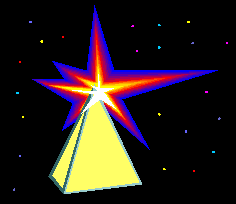
\includegraphics[width=0.5\textwidth]{figures/lots_of_stars.png}
  \end{center}
  \caption{Lots of stars  (Inspired by Figure x.y on page z of [xxx])}
  \label{fig:lotsofstars}
\end{figure}
\sweExpl{Massor av stärnor (Inspirerad av figur x.y på sidan z i [xxx])}


\begin{table}[!ht]
  \begin{center}
    \caption{xxx characteristics}
    \label{tab:tablecaracteristics}
    \begin{tabular}{l|S[table-format=4.6]} % <-- Alignments: 1st column left, 2nd middle, with vertical lines in between
      \textbf{Characteristics} & \textbf{Description}\\
      $\alpha$ & $\beta$ \\
      \hline
      1 & 1110.1\\
      2 & 10.1\\
      3 & 23.113231\\
    \end{tabular}
  \end{center}
\end{table}
\sweExpl{Egenskaper}
\sweExpl{Beskrivning}

\subsection{Subarea 1.1}
Entangled states are an important part of quantum cryptography, but also relevant in other domains. This concept might be relevant for neutrinos, see for example.

\subsection{Subarea 1.1.2}
Computational methods are increasingly used as a third method of carrying out
scientific investigations. For example, computational experiments were used to
find the amount of wear in a polyethylene liner of a hip prosthesis in.
…

\subsection{Subarea 1.1.2}
Using the nearest data center may improve performance


\subsection{Link layer Encapsulation}
\label{sec:llencap}

See Figure~\ref{fig:ieee8023-data-packet} which uses the \textsf{bytefield}  \LaTeX\ package. 


\begin{figure}[!ht]
	\centering
\begin{bytefield}{21}
\bitbox[]{7}{} & \bitbox[]{3}{\tiny octets:} & \bitbox[]{4}{\tiny 6} & \bitbox[]{4}{\tiny 6} & \bitbox[]{3}{\tiny 2} & \bitbox[]{5}{\tiny 46 to 1500} & \bitbox[]{3}{\tiny 0 to 46} & \bitbox[]{2}{\tiny 4}\\ 

\bitbox[]{8}{\textbf{ETHERNET \\[-1ex] \tiny{data link-layer}}} & \bitbox[]{2}{} & 

\bitbox{4}{\tiny Destination Address} & \bitbox{4}{\tiny Source Address} & \bitbox{3}{\tiny Length/ Type} & 
\bitbox{5}{\tiny Data Payload} & \bitbox{3}{\tiny Padding} &
\bitbox{2}{\tiny CRC} \\

\bitbox[]{1}{} &\bitbox[]{3}{\tiny octets:} & \bitbox[]{4}{\tiny 7} & \bitbox[]{2}{\tiny 1} & \bitbox[]{0}{$\vdots$ \\[1ex]} & \bitbox[]{16}{} & \bitbox[]{0}{$\vdots$ \\[1ex]} & \bitbox[]{5}{} & \bitbox[]{4}{\tiny Variable}\\

\bitbox[]{4}{\textbf{MAC \\[-1ex] \tiny{packet}}} & \colorbitbox{lightgray}{4}{\tiny Preamble} & \colorbitbox{lightgray}{2}{\tiny SFD} & \colorbitbox{lightgray}{16}{\tiny MAC Client Data} & \colorbitbox{lightgray}{3}{\tiny Padding} &
\colorbitbox{lightgray}{2}{\tiny CRC} & \colorbitbox{lightgray}{4}{\tiny Extension}
\end{bytefield}
     \caption{Ethernet data link layer protocol encapsulated into a IEEE~802.3 MAC packet}
     \label{fig:ieee8023-data-packet}
\end{figure}

\subsection{IP packet headers}
\label{sec:ipheaders}
The data link layer will receive a packet from the IP layer. The layout of
an IPv4 packet is shown in Figure~\ref{fig:ipv4-header}. This should be
contrasted with the IPv6 header shown in Figure~\ref{fig:ipv6-header}.

%
% IPv4 packet header
%
\begin{figure}[!ht]
	\centering
\begin{bytefield}{32}
\bitheader{0-31} \\
\bitbox{4}{\footnotesize{Version}} & \bitbox{4}{IHL} & \bitbox{6}{\tiny{Type of Service}} & \bitbox{2}{{\scriptsize ECN}} \bitbox{16}{Total Length}\\
\bitbox{16}{Identification} & \bitbox{3}{Flags} & \bitbox{13}{Fragment Offset}\\
\bitbox{8}{Time to Live} & \bitbox{8}{Protocol} & \bitbox{16}{Header Checksum}\\
\wordbox{1}{Source Address}\\
\wordbox{1}{Destination Address}\\
\colorbitbox{lightgray}{24}{Options} & \colorbitbox{lightgray}{8}{Padding}
\end{bytefield}
     \caption[IPv4 datagram header]{IPv4 datagram header. Light grey coloured fields are optional.}
    \label{fig:ipv4-header} 
\end{figure}

%
% IPv6 packet header
%
\begin{figure}[!ht]
	\centering
\begin{bytefield}{32}
\bitheader{0-31} \\
\bitbox{4}{\footnotesize{Version}} & \bitbox{8}{Traffic Class} & \bitbox{20}{Flow Label}\\
\bitbox{16}{Payload Length} & \bitbox{8}{Next Header} & \bitbox{8}{Hop Limit}\\
\wordbox{4}{Source Address}\\
\wordbox{4}{Destination Address}\\
\end{bytefield}
     \caption{IPv6 datagram header}
    \label{fig:ipv6-header}
\end{figure}

\subsection{Test for accessibility of formulas}

As can be seen in these equations:
$c=2 \cdot \pi \cdot r$ or \[ \int_{a}^{b} x^2 \,dx \] a chemical formula: $(C_5O_2H_8)_n$
...
\section{Major background area 2}\sweExpl{Viktigt bakgrundsområde 2}
...
\subsection{WLAN Security}% you can't use the \gls() command in a heading - but you can get the short (\glsentryshort) or long version (\glsentryshort) or \glsentrylong or even the text entry (\glsentrytext) and then there is no problem - see https://tex.stackexchange.com/questions/198140/glossaries-and-custom-section-headings-broken

\subsection{Network layer security}
...

\section{Related work area}\sweExpl{Relaterade arbeten}


\subsection{Major related work 1}\sweExpl{Relaterade arbeten 1}
Carrier clouds have been suggested as a way to reduce the delay between the users and the cloud server that is providing them with content. However, there is a question of how to find the available resources in such a carrier cloud. One approach has been to disseminate resource information using an extension to OSPF-TE, see Roozbeh, Sefidcon, and Maguire.


\subsection{Major related work n}\sweExpl{Relaterade arbeten}

\subsection{Minor related work 1}\sweExpl{Mindre relaterat arbete 1}


…
\subsection{Minor related work n}\sweExpl{Mindre relaterat arbete n}


\section{Summary}\sweExpl{Sammanfattning}
\sweExpl{Det är trevligt om detta kapitel
  avslutas med en sammanfattning. Till exempel kan du inkludera en tabell som
  sammanfattar andras idéer och fördelar och nackdelar med varje - så som
  senare kan du jämföra din lösning till var och en av dessa. Detta kommer
  också att hjälpa dig att definiera de variabler som du kommer att använda
  för din utvärdering.}

\engExpl{It is nice to have this chapter conclude with a summary. For
  example, you can include a table that summarizes other people's ideas and
  benefits and drawbacks with each - so as later you can compare your solution
  to each of them. This will also help you define the variables that you will
  use for your evaluation.}

\cleardoublepage

\chapter{Method}
    \label{ch:method}
    \sweExpl{Metod eller Metodval}
\generalExpl{This chapter is about Engineering-related
  content, Methodologies and Methods.  Use a self-explaining title.\\The
  contents and structure of this chapter will change with your choice of
  methodology and methods.}


\generalExpl{Describe the engineering-related contents (preferably with models) and the research methodology and methods that are used in the degree project.\\
Give a theoretical description of the scientific or engineering methodology  you are going to use and why have you chosen this method. What other methods did you consider and why did you reject them?\\
In this chapter, you describe what engineering-related and scientific skills you are going to apply, such as modeling, analyzing, developing, and evaluating engineering-related and scientific content. The choice of these methods should be appropriate for the problem. Additionally, you should be conscious of aspects relating to society and ethics (if applicable). The choices should also reflect your goals and what you (or someone else) should be able to do as a result of your solution - which could not be done well before you started.}

The purpose of this chapter is to provide an overview of the research method
used in this thesis. Section~\ref{sec:researchProcess} describes the research
process. Section~\ref{sec:researchParadigm} details the research
paradigm. Section~\ref{sec:dataCollection} focuses on the data collection
techniques used for this research. Section~\ref{sec:experimentalDesign}
describes the experimental design. Section~\ref{sec:assessingReliability}
explains the techniques used to evaluate the reliability and validity of the
data collected. Section~\ref{sec:plannedDataAnalysis} describes the method
used for the data analysis. Finally, Section~\ref{sec:evaluationFramework}
describes the framework selected to evaluate xxx.

\sweExpl{Vilka vetenskaplig eller ingenjörs-metodik ska du använda och varför har du valt den här metoden. Vilka andra metoder gjorde du övervägde du och varför du avvisar dem.
Vad är dina mål? (Vad ska du kunna göra som ett resultat av din lösning - vilken inte kan göras i god tid innan du började)
Vad du ska göra? Hur? Varför? Till exempel, om du har implementerat en artefakt vad gjorde du och varför? Hur kommer du utvärdera den.
Syftet med detta kapitel är att ge en översikt över forsknings metod som
används i denna avhandling. Avsnitt~\ref{sec:researchProcess} beskriver forskningsprocessen. Avsnitt~\ref{sec:researchParadigm} beskriver forskningsparadigmen detaljerat. Avsnitt~\ref{sec:dataCollection} fokuserar på datainsamlingstekniker som används för denna forskning. Avsnitt~\ref{sec:experimentalDesign} beskriver experimentell
design. Avsnitt~\ref{sec:assessingReliability} förklarar de tekniker som används för att utvärdera
tillförlitligheten och giltigheten av de insamlade uppgifterna. Avsnitt~\ref{sec:plannedDataAnalysis}
beskriver den metod som används för dataanalysen. Slutligen, Avsnitt~\ref{sec:evaluationFramework}
beskriver ramverket som valts för att utvärdera xxx.\\
Ofta kan man koppla ett antal följdfrågor till undersökningsfrågan och problemlösningen t ex\\
(1) Vilken process skall användas för konstruktion av lösningen och vilken process skall kopplas till denna för att svara på undersökningsfrågan?\\
(2) Hur och vilket resultat (storheter) skall presenteras både för att redovisa svar på undersökningsfrågan (resultatkapitlet i denna rapport) och redovisa resultat av problemlösningen (prototypen, ofta dokument som bilagor men vilka dokument och varför?).\\
(3) Vilken teori/teknik skall väljas och användas både för undersökningen (taxonomi, matematik, grafer, storheter mm)  och  problemlösning (UML, UseCases, Java mm) och varför?\\
(4) Vad behöver du som student leverera för att uppnå hög kvaliet (minimikrav) eller mycket hög kvalitet på examensarbetet?\\
(5) Frågorna kopplar till de följande underkapitlen.\\
(6) Resonemanget bygger på att studenter på hing-programmet ofta skall konstruera något åt problemägaren och att man till detta måste koppla en intressant ingenjörsfråga. Det finns hela tiden en dualism mellan dessa aspekter i exjobbet.
}

\section{Research Process}
\label{sec:researchProcess}

\sweExpl{Undersökningsrocess och utvecklingsprocess}

Figure~\ref{fig:researchprocess} shows the steps conducted to carry out this research. 

\sweExpl{Figur~\ref{fig:researchprocess} visar de steg som utförs för att genomföra\\
Beskriv, gärna med ett aktivitetsdiagram (UML?), din undersökningsprocess och utvecklingsprocess.  Du måste koppla ihop det akademiska intresset (undersökningsprocess) med ursprungsproblemet (utvecklingsprocess)
denna forskning.\\
Aktivitetsdiagram från t ex UML-standard}


 
\begin{figure}[!ht]
  \begin{center}
    
\includegraphics[width=0.5\textwidth]{figures/researchprocess.png}
  \end{center}
  \caption{Research Process}
  \label{fig:researchprocess}
\end{figure}

\generalExpl{Example of using customized item labels.}
Some steps in the process:
\begin{enumerate}[leftmargin=*, label=\textbf{Step \arabic*}, ref=Step \arabic*] %labelindent=1em for indent
    \itemsep0em
    \item \label{x:s1} plan experiment,
    \item \label{x:s2} conduct experiment,
    \item \label{x:s3} analyze data from the experiment, and
    \item \label{x:s4} discuss the results of the analysis.
\end{enumerate}

\sweExpl{Forskningsprocessen}


\section{Research Paradigm}
\label{sec:researchParadigm}
\sweExpl{Undersökningsparadigm\\
\section{Data Collection}
\label{sec:dataCollection}
\sweExpl{Datainsamling\\
(Detta bör också visa att du är medveten om de sociala och etiska frågor som
kan vara relevanta för dina data insamlingsmetod.)}
\generalExpl{This should also show that you are aware of the social and ethical concerns that might be relevant to your data collection method.}



\subsection{Sampling}
\sweExpl{Stickprovsundersökning}

\subsection{Sample Size}
\sweExpl{Provstorleken}

\subsection{Target Population}
\sweExpl{Målgruppen}

\section[Experimental design/Planned Measurements]{Experimental design and\\Planned Measurements}
\label{sec:experimentalDesign}
\sweExpl{Experimentdesign/Mätuppställning}

\subsection{Test environment/test bed/model}
\engExpl{Describe everything that someone else would need to reproduce your test environment/test bed/model/… .}
\sweExpl{Testmiljö/testbädd/modell\\
Beskriv allt att någon annan skulle behöva återskapa din testmiljö / testbädd / modell / …}

\subsection{Hardware/Software to be used}
\sweExpl{Hårdvara / programvara som ska användas}


\section{Assessing reliability and validity of the data collected}
\label{sec:assessingReliability}
\sweExpl{Bedömning av validitet och reliabilitet hos använda metoder och insamlade data }


\subsection{Validity of method}
\label{sec:validtyOfMethod}
\sweExpl{Giltigheten av metoder\\
  Har dina metoder gett dig de rätta svaren och lösningarna? Var metoderna korrekta?}

\engExpl{How will you know if your results are valid?}
\engExpl{Remember that validity is about the \textit{accuracy} of a measurement while reliability is about the \textit{consistency} of the measurement values under the same conditions (\ie repeatability).}

\subsection{Reliability of method}
\label{sec:reliabilityOfMethod}
\sweExpl{Tillförlitlighet av för metoder\\
Hur bra är dina metoder, finns det bättre metoder? Hur kan du förbättra dem?}
\engExpl{How will you know if your results are reliable?}

\subsection{Data validity}
\label{sec:dataValidity}
\sweExpl{Giltigheten av uppgifter\\
Hur vet du om dina resultat är giltiga? Är ditt resultat rättvisande?}

\subsection{Reliability of data}
\label{sec:reliabilityOfData}
\sweExpl{Tillförlitlighet av data\\
Hur vet du om dina resultat är tillförlitliga? Hur bra är dina resultat?}


\section{Planned Data Analysis}
\label{sec:plannedDataAnalysis}
\sweExpl{Metod för analys av data}


\subsection{Data Analysis Technique}
\label{sec:dataAnalysisTechnique}
\sweExpl{Dataanalysteknik}

\subsection{Software Tools}
\label{sec:softwareTools}
\sweExpl{Mjukvaruverktyg}


\section{Evaluation framework}
\label{sec:evaluationFramework}
\sweExpl{Utvärdering och ramverk\\
Metod för utvärdering, jämförelse mm. Kopplar till kapitel~\ref{ch:resultsAndAnalysis}.}

\section{System documentation}
\label{sec:systemDocumentation}
\sweExpl{Systemdokumentation\\
Med vilka dokument och hur skall en konstruerad prototyp dokumenteras? Detta blir ofta bilagor till rapporten och det som problemägaren till det ursprungliga problemet (industrin) ofta vill ha.\\
Bland dessa bilagor återfinns ofta, och enligt någon angiven standard, kravdokument, arkitekturdokument, designdokumnet, implementationsdokument, driftsdokument, testprotokoll mm.}
\generalExpl{If this is going to be a complete document consider putting it in as an appendix, then just put the highlights here.}

\cleardoublepage

\chapter{Implementation}\engExpl{Choose your own chapter title to describe this}
    \label{ch:implementation}
    \sweExpl{[Vad gjorde du? Hur gick det till? – Välj lämplig rubrik (“Genomförande”, “Konstruktion”, ”Utveckling”  eller annat]}


\engExpl{What have you done? How did you do it? What design decisions did you make? How did what you did help you to meet your goals?}
\sweExpl{Vad du har gjort? Hur gjorde du det? Vilka designval gjorde du?\\
Hur kom det du hjälpte dig att uppnå dina mål?}

% the following sets the TOC entry to break after the & - note you have to include the first letter of the following word as it get swolled by the \texorpdfstring{}{} processing
\section[Hardware/Software design …/Model/Simulation model \&\texorpdfstring{\\}{ p} parameters/…]{Hardware/Software design …/Model/Simulation model \& parameters/…}
\sweExpl{Hårdvara / Mjukvarudesign ... / modell / Simuleringsmodell och parametrar / …}

Figure~\ref{fig:homepageicon} shows a simple icon for a home page. The time
to access this page when served will be quantified in a series of
experiments. The configurations that have been tested in the test bed are
listed in Table~\ref{tab:configstested}. In \SI{7.0}{\percent} of cases, there was an error indicating xxxxx.

\sweExpl{Figur~\ref{fig:homepageicon}  visar en enkel ikon för en hemsida. Tiden för att få tillgång till den här sidan när den laddas kommer att kvantifieras i en serie experiment. De konfigurationer som har testats i provbänk listas ini tabell~\ref{tab:configstested}.\\
Vad du har gjort? Hur gjorde du det? Vilka designval gjorde du?}
 
\begin{figure}[!ht]
  \begin{center}
    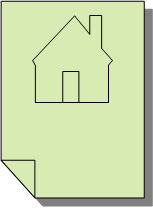
\includegraphics[width=0.25\textwidth]{figures/Homepage-icon.png}
  \end{center}
  \caption{Homepage icon}
  \label{fig:homepageicon}
\end{figure}

\begin{table}[!ht]
  \begin{center}
    \caption{Configurations tested}
    \label{tab:configstested}
    \resizebox{\columnwidth}{!}{%
    \begin{tabular}{l|c} % <-- Alignments: 1st column left, 2nd middle and 3rd right, with vertical lines in between
      \textbf{Configuration} & \textbf{Description} \\
      \hline
      1 & Simple test with one server\\
      2 & Simple test with one server\\
    \end{tabular}
    }
  \end{center}
\end{table}
\sweExpl{Testade konfigurationer}

\section{Implementation …/Modeling/Simulation/…}
\label{sec:implementationDetails}
\sweExpl{Implementering … / modellering / simulering / …}

Two commonly used simulators are:
\begin{description}[labelwidth =\widthof{\textbf{ns-2 or ns-3 simulator}}, leftmargin = !]
    \item[\textbf{Mininet}] This simulator uses traffic control (\texttt{tc}) to simulate network devices connected by links with specific bandwidth, packet loss rates, qdisc methods, etc.
    
    
    \item[\textbf{ns-2 or ns-3 simulator}] These simulators are very useful for simulating wireless communication links between moving devices. You can specify the mobility patterns of the nodes.
\end{description}

\subsection{Some examples of coding}
\engExpl{This section is simply to show some example of how you can include code in your thesis - this is not a section you would have in your thesis.}
\sweExpl{Det här avsnittet är helt enkelt för att visa ett exempel på hur du kan inkludera kod i ditt examensarbete - det här är inte ett avsnitt du skulle ha i ditt examensarbete.}

Listing~\ref{lst:helloWorldInC} shows an example of a simple program written
in C code.

\begin{lstlisting}[language={C}, caption={Hello world in C code}, label=lst:helloWorldInC]
int main() {
printf("hello, world");
return 0;
}
\end{lstlisting}


In contrast, Listing~\ref{lst:programmes} is an example of code in Python to
get a list of all of the programs at KTH.

\lstset{extendedchars=true}  %% This allows characters codes in the range 128-255
\begin{lstlisting}[language={Python}, caption={Using a python program to
    access the KTH API to get all of the programs at KTH}, label=lst:programmes]
KOPPSbaseUrl = 'https://www.kth.se'

def v1_get_programmes():
    global Verbose_Flag
    #
    # Use the KOPPS API to get the data
    # note that this returns XML
    url = "{0}/api/kopps/v1/programme".format(KOPPSbaseUrl)
    if Verbose_Flag:
        print("url: " + url)
    #
    r = requests.get(url)
    if Verbose_Flag:
        print("result of getting v1 programme: {}".format(r.text))
    #
    if r.status_code == requests.codes.ok:
        return r.text           # simply return the XML
    #
    return None
\end{lstlisting}
\FloatBarrier

\subsection{Some examples of figures in tikz}
\engExpl{This section is simply to show some example of how you can draw your own figures for in your thesis - this is not a section you would have in your thesis.}
\sweExpl{Det här avsnittet är helt enkelt för att visa ett exempel på hur du kan rita dina egna figurer i ditt examensarbete – det här är inte ett avsnitt du skulle ha i ditt examensarbete.}

These figures are just some examples to show that you can draw your own figures for in your thesis. This has two advantages: \first you do not have to worry about copyrights -- as these are your own figures and \Second the text is now readable and not simply a picture of text -- so screen readers can read the figure's contents to someone who is listening to the contents of your thesis.

\subsubsection{Azure's Form Recognizer}
\Cref{fig:processAnInvoice} shows the processing of key-value extraction from a PDF document using Azure's Form Recognizer. 

\tikzset{
    processBox/.style={rectangle, rounded corners, minimum width=3cm, minimum height=1cm,text centered, font=\sffamily, draw=black, fill=red!20},
    largeBox/.style={rectangle, rounded corners, minimum width=3cm, minimum height=4cm,text centered, draw=black}
}
\begin{figure}[!ht]
\resizebox{1.1\textwidth}{!}{%
\begin{tikzpicture}
[align=left,node distance=2cm]

\node (document) [tape,tape bend top=none,draw,font=\sffamily] {PDF\\Document};
\node (GDM) [processBox,  right=0.5cm of document] {OCR};
\node (OCRoutput) [largeBox, right=1cm of GDM] {OCR output};

\node (kvp) [tape,tape bend top=none,draw,font=\sffamily, below=0.25cm of OCRoutput.north] {key-value\\pairs};
\node (entities) [tape,tape bend top=none,draw,font=\sffamily, above=0.35cm of OCRoutput.south] {Entities};
\node (Manual) [processBox, right=1cm of kvp] {Analyze the extracted\\key-value pairs};
\draw [-latex](document) --  (GDM);
\draw [-latex](kvp) --  (Manual);
\path[ draw
     , -latex'] let \p1=(GDM.east), \p2=(kvp.west) in (GDM.east) -- +(0.25*\x2-0.25*\x1, \y1) -- +(0.5*\x2-0.5*\x1, \y2) -- (kvp.west);
\path[ draw
     , -latex'] let \p1=(GDM.east), \p2=(kvp.west), \p3=(entities.west) in (GDM.east) --  +(0.25*\x2-0.25*\x1, \y1) -- +(0.5*\x3-0.5*\x1, \y3) -- (entities.west);
\end{tikzpicture}
}
\caption{The processing of key-value extraction from a PDF document using Azure's Form Recognizer}
  \label{fig:processAnInvoice}
\end{figure}
\FloatBarrier
\subsubsection{Hyper-V with Containers}
 \Cref{fig:hyperVcontainers} shows how Hyper-V deals with containers.
 
 \tikzset{
    container/.style={rectangle, rounded corners, minimum width=2cm, minimum height=1cm,text centered, draw=black, fill=blue!20},
    containerization/.style={rectangle, rounded corners, minimum width=13.25cm, minimum height=1cm,text centered, draw=black, fill=blue!20},
    hypervisor/.style={rectangle, rounded corners, minimum width=13.25cm, minimum height=1cm,text centered, draw=black, fill=red!20},
    os/.style={rectangle, rounded corners, minimum width=13.25cm, minimum height=1cm,text centered, draw=black, fill=orange!20},
    guestos/.style={rectangle, rounded corners, minimum width=2cm, minimum height=1cm,text centered, draw=black, fill=orange!40},
    infrastructure/.style={rectangle, rounded corners, minimum width=13.25cm, minimum height=1cm,text centered, draw=black, fill=green!20},
    hos/.style={rectangle, rounded corners, minimum width=6cm, minimum height=1cm,text centered, draw=black, fill=orange!20},
    kernel/.style={rectangle, rounded corners, minimum width=6cm, minimum height=1cm,text centered, draw=black, fill=purple!20},
    services/.style={rectangle, rounded corners, minimum width=3cm, minimum height=1cm,text centered, draw=black, fill=pink!20]}
}

\begin{figure}[ht!]
    \centering
\resizebox{1\textwidth}{!}{%
\begin{tikzpicture}
[align=center,node distance=2cm]

\node (Infrastructure) [infrastructure, text width=13cm, text centered] {Infrastructure};
\node (OS1) [hos, anchor=north west, align=left, above=1.5cm of Infrastructure.north west, anchor=north west, text width=6cm, text centered] {Host OS};

\node (OS2) [hos, anchor= west, align=left, right=0.5cm of OS1.east, text width=6cm, anchor= west, text centered] {Host OS};

\node (Kernel1) [kernel, anchor=north west, align=left, above=1.5cm of OS1.north east, anchor=north east, text width=3cm, text centered] {Kernel};

\node (Kernel2) [kernel, anchor=north west, align=left, above=1.5cm of OS2.north east, anchor=north east, text width=3cm, text centered] {Kernel};

\node (ServiceA) [container, anchor=east, above=1 cm of Kernel1.east, anchor=east] {Services};
\node (AppA) [container,  left=0.25cm of ServiceA] {App 1};

\node (ServiceB) [container, anchor=east, above=1 cm of Kernel2.east, anchor=east] {Services};
\node (AppB) [container,  left=0.25cm of ServiceB] {App 2};
%\node (AppC) [container,  right=0.25cm of AppB] {App 3};

\draw[black,thick,dashed] ($(OS2.north west)+(-0.3,3.75)$)  rectangle ($(OS2.south east)+(0.5,-0.3)$);
\node[text width=5cm, text=red, above=0.1cm of ServiceB] 
    {\textbf{Container}};

\draw[red,thick,dotted] ($(Kernel2.north west)+(-0.3,1.6)$)  rectangle ($(Kernel2.south east)+(0.3,-0.3)$);
\node[text width=5cm, text=black, above=0.8cm of ServiceB] 
    {\textbf{VM}};
\end{tikzpicture}
}
    \caption{Hyper-V with containers}
    \label{fig:hyperVcontainers}
\end{figure}
\FloatBarrier
\subsubsection{VM versus Containers}
\Cref{fg:vmsVersusContainers} shows a comparison of virtual machines (VMs) versus containers.

\begin{figure*}[ht!]
    \centering
    \begin{subfigure}[t]{0.5\textwidth}
        \centering
\resizebox{1\textwidth}{!}{%
\begin{tikzpicture}
[align=left,node distance=2cm]

\node (AppA) [container,align=left] {App 1};
\node (AppB) [container,  right=0.25cm of AppA] {App 2};
\node (AppC) [container,  right=0.25cm of AppB] {App 3};

\node (GosA) [guestos,align=left,  below=0.25cm of AppA.south west,anchor=north west] {Guest OS};
\node (GosB) [guestos,  right=0.25cm of GosA] {Guest OS};
\node (GosC) [guestos,  right=0.25cm of GosB] {Guest OS};

\draw [decoration={brace,amplitude=0.5em},decorate, ultra thick,gray, transform canvas={xshift = 0.5cm}]
       (AppC.north -| AppC.east) -- (GosC.south -| AppC.east);
\node[text width=5cm,  right=1cm of GosC.north east] 
    {\textbf{VMs}};

\node (Hypervisor) [hypervisor, anchor=north west, align=left, below=0.25cm of GosA.south west, anchor=north west, text width=13cm, text centered] {Hypervisor};

\node (OS) [os, anchor=north west, align=left, below=0.25cm of Hypervisor.south west, anchor=north west, text width=13cm, text centered] {Host OS};

\node (Infrastructure) [infrastructure, anchor=north west, align=left, below=0.25cm of OS.south west, anchor=north west, text width=13cm, text centered] {Infrastructure};


\end{tikzpicture}
}
        \caption{VM}
    \end{subfigure}%
    ~ 
    \begin{subfigure}[t]{0.5\textwidth}
        \centering
        \resizebox{1\textwidth}{!}{%
\begin{tikzpicture}
[align=left,node distance=2cm]

\node (AppA) [container,align=left] {App 1};
\node (AppB) [container,  right=0.25cm of AppA] {App 2};
\node (AppC) [container,  right=0.25cm of AppB] {App 3};
\node[text width=5cm,  right=0.25cm of AppC] 
    {\textbf{Apps running in Containers}};


\node (Containerization) [containerization, anchor=north west, align=left, below=0.25cm of AppA.south west, anchor=north west, text width=13cm, text centered] {Docker Engine};

\node (OS) [os, anchor=north west, align=left, below=0.25cm of Containerization.south west, anchor=north west, text width=13cm, text centered] {Host OS};

\node (Infrastructure) [infrastructure, anchor=north west, align=left, below=0.25cm of OS.south west, anchor=north west, text width=13cm, text centered] {Infrastructure};


\end{tikzpicture}
}
        \caption{Containers}
    \end{subfigure}
    \caption{Virtual machines (VMs) versus Containers}
    \label{fg:vmsVersusContainers}
\end{figure*}


\cleardoublepage

\chapter{Results and Analysis}
    \label{ch:results_and_analysis}
    \sweExpl{svensk: Resultat och Analys}

\engExpl{Sometimes this is split into two chapters.\\Keep in mind: How you are going to evaluate what you have done? What are your metrics?\\Analysis of your data and proposed solution\\Does this meet the goals which you had when you started?}

In this chapter, we present the results and discuss them.

\sweExpl{I detta kapitel presenterar vi resultaten och diskutera dem.\\Ibland delas detta upp i två kapitel.\\Hur du ska utvärdera vad du har gjort? Vad är din statistik?\\Analys av data och föreslagen lösning\\Innebär detta att uppfyllelse av de mål som du hade när du började?}

\section{Major results}
\sweExpl{Huvudsakliga resultat}

Some statistics of the delay measurements are shown in Table~\ref{tab:delayMeasurements}.
The delay has been computed from the time the GET request is received until the response is sent.

\sweExpl{Lite statistik av fördröjningsmätningarna visas i Tabell~\ref{tab:delayMeasurements}. Förseningen har beräknats från den tidpunkt då begäran GET tas emot fram till svaret skickas.}

\begin{table}[!ht]
  \begin{center}
    \caption{Delay measurement statistics}
    \label{tab:delayMeasurements}
    \begin{tabular}{l|S[table-format=4.2]|S[table-format=3.2]} % <-- Alignments: 1st column left, 2nd middle and 3rd right, with vertical lines in between
      \textbf{Configuration} & \textbf{Average delay (ns)} & \textbf{Median delay (ns)}\\
      \hline
      1 & 467.35 & 450.10\\
      2 & 1687.5 & 901.23\\
    \end{tabular}
  \end{center}
\end{table}

Table \ref{tab:ping_results} shows the measurement of round trip times from four hosts to and from a server.
\begin{table}[ht!]
\caption[RTT for 4 hosts]{Result for the ping measurements of RTT for 4 hosts} 
\label{tab:ping_results}
\vspace{1em}
\centering
\begin{tabular}{l *{4}{S[table-format=2.3]}}
{} & \multicolumn{4}{c}{host to server RTT in ms} \\
\cmidrule{2-5}
Host & \multicolumn{1}{c}{min}  & \multicolumn{1}{c}{avg} & \multicolumn{1}{c}{max} & \multicolumn{1}{c}{mdev} \\
\midrule
h1 & 5.625 & 5.625 & 5.625 & 0.0 \\
h2 & 2.909 & 2.909 & 1.909 & 0.0 \\
h3 & 5.007 & 5.007 & 5.007 & 0.0 \\
h4 & 2.308 & 2.308 & 2.308 & 0.0 \\
\midrule
\end{tabular}
\end{table}
\FloatBarrier

\sweExpl{Fördröj mätstatistik}
\sweExpl{Konfiguration | Genomsnittlig fördröjning (ns) | Median fördröjning (ns)}

Figure \ref{fig:processing_vs_payload_length} shows an example of the performance as measured in the experiments.

\begin{figure}[!ht]
% GNUPLOT: LaTeX picture
\setlength{\unitlength}{0.240900pt}
\ifx\plotpoint\undefined\newsavebox{\plotpoint}\fi
\begin{picture}(1500,900)(0,0)
\sbox{\plotpoint}{\rule[-0.200pt]{0.400pt}{0.400pt}}%
\put(171.0,131.0){\rule[-0.200pt]{4.818pt}{0.400pt}}
\put(151,131){\makebox(0,0)[r]{ 1.5}}
\put(1419.0,131.0){\rule[-0.200pt]{4.818pt}{0.400pt}}
\put(171.0,212.0){\rule[-0.200pt]{4.818pt}{0.400pt}}
\put(151,212){\makebox(0,0)[r]{ 2}}
\put(1419.0,212.0){\rule[-0.200pt]{4.818pt}{0.400pt}}
\put(171.0,292.0){\rule[-0.200pt]{4.818pt}{0.400pt}}
\put(151,292){\makebox(0,0)[r]{ 2.5}}
\put(1419.0,292.0){\rule[-0.200pt]{4.818pt}{0.400pt}}
\put(171.0,373.0){\rule[-0.200pt]{4.818pt}{0.400pt}}
\put(151,373){\makebox(0,0)[r]{ 3}}
\put(1419.0,373.0){\rule[-0.200pt]{4.818pt}{0.400pt}}
\put(171.0,454.0){\rule[-0.200pt]{4.818pt}{0.400pt}}
\put(151,454){\makebox(0,0)[r]{ 3.5}}
\put(1419.0,454.0){\rule[-0.200pt]{4.818pt}{0.400pt}}
\put(171.0,534.0){\rule[-0.200pt]{4.818pt}{0.400pt}}
\put(151,534){\makebox(0,0)[r]{ 4}}
\put(1419.0,534.0){\rule[-0.200pt]{4.818pt}{0.400pt}}
\put(171.0,615.0){\rule[-0.200pt]{4.818pt}{0.400pt}}
\put(151,615){\makebox(0,0)[r]{ 4.5}}
\put(1419.0,615.0){\rule[-0.200pt]{4.818pt}{0.400pt}}
\put(171.0,695.0){\rule[-0.200pt]{4.818pt}{0.400pt}}
\put(151,695){\makebox(0,0)[r]{ 5}}
\put(1419.0,695.0){\rule[-0.200pt]{4.818pt}{0.400pt}}
\put(171.0,776.0){\rule[-0.200pt]{4.818pt}{0.400pt}}
\put(151,776){\makebox(0,0)[r]{ 5.5}}
\put(1419.0,776.0){\rule[-0.200pt]{4.818pt}{0.400pt}}
\put(171.0,131.0){\rule[-0.200pt]{0.400pt}{4.818pt}}
\put(171,90){\makebox(0,0){ 0}}
\put(171.0,756.0){\rule[-0.200pt]{0.400pt}{4.818pt}}
\put(298.0,131.0){\rule[-0.200pt]{0.400pt}{4.818pt}}
\put(298,90){\makebox(0,0){ 10}}
\put(298.0,756.0){\rule[-0.200pt]{0.400pt}{4.818pt}}
\put(425.0,131.0){\rule[-0.200pt]{0.400pt}{4.818pt}}
\put(425,90){\makebox(0,0){ 20}}
\put(425.0,756.0){\rule[-0.200pt]{0.400pt}{4.818pt}}
\put(551.0,131.0){\rule[-0.200pt]{0.400pt}{4.818pt}}
\put(551,90){\makebox(0,0){ 30}}
\put(551.0,756.0){\rule[-0.200pt]{0.400pt}{4.818pt}}
\put(678.0,131.0){\rule[-0.200pt]{0.400pt}{4.818pt}}
\put(678,90){\makebox(0,0){ 40}}
\put(678.0,756.0){\rule[-0.200pt]{0.400pt}{4.818pt}}
\put(805.0,131.0){\rule[-0.200pt]{0.400pt}{4.818pt}}
\put(805,90){\makebox(0,0){ 50}}
\put(805.0,756.0){\rule[-0.200pt]{0.400pt}{4.818pt}}
\put(932.0,131.0){\rule[-0.200pt]{0.400pt}{4.818pt}}
\put(932,90){\makebox(0,0){ 60}}
\put(932.0,756.0){\rule[-0.200pt]{0.400pt}{4.818pt}}
\put(1059.0,131.0){\rule[-0.200pt]{0.400pt}{4.818pt}}
\put(1059,90){\makebox(0,0){ 70}}
\put(1059.0,756.0){\rule[-0.200pt]{0.400pt}{4.818pt}}
\put(1185.0,131.0){\rule[-0.200pt]{0.400pt}{4.818pt}}
\put(1185,90){\makebox(0,0){ 80}}
\put(1185.0,756.0){\rule[-0.200pt]{0.400pt}{4.818pt}}
\put(1312.0,131.0){\rule[-0.200pt]{0.400pt}{4.818pt}}
\put(1312,90){\makebox(0,0){ 90}}
\put(1312.0,756.0){\rule[-0.200pt]{0.400pt}{4.818pt}}
\put(1439.0,131.0){\rule[-0.200pt]{0.400pt}{4.818pt}}
\put(1439,90){\makebox(0,0){ 100}}
\put(1439.0,756.0){\rule[-0.200pt]{0.400pt}{4.818pt}}
\put(171.0,131.0){\rule[-0.200pt]{0.400pt}{155.380pt}}
\put(171.0,131.0){\rule[-0.200pt]{305.461pt}{0.400pt}}
\put(1439.0,131.0){\rule[-0.200pt]{0.400pt}{155.380pt}}
\put(171.0,776.0){\rule[-0.200pt]{305.461pt}{0.400pt}}
\put(30,453){\rotatebox{-270}{\makebox(0,0){Processing time (ms)}}}
\put(805,29){\makebox(0,0){Payload size (bytes)}}
\put(868.0,131.0){\rule[-0.200pt]{0.400pt}{84.074pt}}
\put(995.0,131.0){\rule[-0.200pt]{0.400pt}{98.287pt}}
\put(1173.0,131.0){\rule[-0.200pt]{0.400pt}{118.041pt}}
\put(1325.0,131.0){\rule[-0.200pt]{0.400pt}{134.904pt}}
\put(1350.0,131.0){\rule[-0.200pt]{0.400pt}{137.795pt}}
\put(1439.0,131.0){\rule[-0.200pt]{0.400pt}{155.380pt}}
\end{picture}
\caption[A GNUplot figure]{Processing time vs. payload length}\vspace{0.5cm}
\label{fig:processing_vs_payload_length}
\end{figure}
\FloatBarrier		

Given these measurements, we can calculate our processing bit rate as the inverse of the time it takes to process an additional byte divided by 8 bits per byte:

\[
	\text{bit rate} = \frac{1}{\frac{\text{time}_{\text{byte}}}{8}} = 20.03 \quad kb/s
\] 

\Cref{tab:majorMarkupLMDetailedResult} shows another table in which some values have been set in bold (using \textbackslash B) to emphasize them. Note how the \texttt{S} formatting has been modified so that it considers the weight of the characters and this is able to decimal align even these hold-faced numbers with the numbers in the column above them.

\begin{table}[!ht]
    \centering
    \caption{Median values of sandwich attributes}
    \label{tab:majorMarkupLMDetailedResult}
    \begin{tabular}{l *{2}{S[detect-weight,mode=text,table-format=3.2]}}
        & \multicolumn{2}{c}{\textbf{sites}}\\
        \cmidrule{2-3}
        \textbf{Attribute} & \textbf{A} & \textbf{B} \\
        \midrule
        price (in SEK) & 36.5 & 71.3 \\
        protean (g) & 97.2 & 100.0 \\
        salt (mg) & 9.7 & 9.3 \\
        \hline
        \textbf{Average customer rating in \%} & \B 82.2 & \B 89.9 \\
        \midrule
    \end{tabular}
\end{table}
\FloatBarrier


\Needspace*{4\baselineskip}
\Cref{fig:stackedrust} shows a stacked bar chart using pgfplots. It illustrates how easy it is to take a set of data and make a stacked bar plot. One of the features is the shifted values -- this is very useful when the bar itself is too small to put the value into.

\pgfplotstableread{
Label Numbers  Refs  Struct/Enum  Heap  Arrays
cratesio 70.04 19.83 8.31 1.3 0.52
librs 49.26 30.49 10.80 7.92 1.53
rustc 55.01 24.80 11.54 6.16 2.49
}\testdata


\pgfkeys{
    /pgf/number format/.cd,
    fixed,
    fixed zerofill,
    precision=2
}
\begin{figure}[ht!]
    \centering
    \scalebox{0.9}{
    \begin{tikzpicture}
    \begin{axis}[
        ybar stacked,
        %reverse legend,
        reverse legend=false,
        %https://tex.stackexchange.com/questions/88892/pgfplots-bar-plot-spacing-inbetween-bars
        enlarge x limits=0.4,
	    bar width=45pt,
        /pgfplots/nodes near coords*/.append style={
        every node near coord/.style={
            color=black,
            font=\small,
            name=X,
%            shift={    
%                (50pt,25pt)
%                },
            xshift={50pt},
                yshift ={
                ifthenelse((\plotnum == 4), 30pt,20pt)},
            },
            scatter/@post marker code/.append code={
                \node(Y){};
                \draw(X)--(Y.center);
            }
        },
	    nodes near coords,
        bar shift=5pt,
        ymin=0,
        ymax=115,
        xtick=data,
        width=1\textwidth,
        legend style={draw=none},
        legend image post style={scale=2.0},
        legend style={
            at={(0.5,-0.2)},
            anchor=north,
            legend columns=-2,
            font=\large,
            %mark size=20pt,
        },
        ylabel=Percentage points (\%),
        xticklabels from table={\testdata}{Label},
        xticklabel style={rotate=30},
    ]
    \addplot  table [y=Numbers, meta=Label, x expr=\coordindex] {\testdata};
    \addlegendentry{Numbers}
    \addplot table [y=Refs, meta=Label, x expr=\coordindex] {\testdata};
    \addlegendentry{Refs}
    \addplot  table [y=Struct/Enum, meta=Label, x expr=\coordindex] {\testdata};
    \addlegendentry{Struct/Enum}
    \addplot  table [y=Heap, meta=Label, x expr=\coordindex] {\testdata};
    \addlegendentry{Heap}
    \addplot  table [y=Arrays, meta=Label, x expr=\coordindex] {\testdata};
    \addlegendentry{Arrays}
    \end{axis}
    \end{tikzpicture}}
\caption{Rust types distribution for the compiler, crates.io, and lib.rs.
(percentage) - appears here with the permission of the author - see the thesis at \url{https://urn.kb.se/resolve?urn=urn\%3Anbn\%3Ase\%3Akth\%3Adiva-332124}}
\label{fig:stackedrust}
\end{figure}
\FloatBarrier



\section{Reliability Analysis}
\sweExpl{Analys av tillförlitlighet\\
Tillförlitlighet i metod och data}

\section{Validity Analysis}
\sweExpl{Analys av validitet\\
Validitet i metod och data}

\cleardoublepage
\chapter{Discussion}
\label{ch:discussion}
\sweExpl{Diskussion\\
Förbättringsförslag?}
\generalExpl{This can be a separate chapter or a section in the previous chapter.}

\cleardoublepage

\chapter{Conclusions and Future work}
    \label{ch:conclusions_and_future_work}
    \sweExpl{Slutsats och framtida arbete}

\generalExpl{Add text to introduce the subsections of this chapter.}

\section{Conclusions}
\label{sec:conclusions}
\sweExpl{Slutsatser}
\engExpl{Describe the conclusions (reflect on the whole introduction given in Chapter 1).}


  
\engExpl{Discuss the positive effects and the drawbacks.\\
Describe the evaluation of the results of the degree project.\\
Did you meet your goals?\\
What insights have you gained?\\
What suggestions can you give to others working in this area?\\
If you had it to do again, what would you have done differently?}

\sweExpl{Uppfyllde du dina mål?\\
Vilka insikter har du fått?\\
Vilka förslag kan du ge till andra som arbetar inom detta område?
Om du skulle göra detta igen, vad skulle du ha gjort annorlunda?}

\section{Limitations}
\label{sec:limitations}
\sweExpl{Begränsande faktorer\\Vad gjorde du som begränsade dina ansträngningar? Vilka är begränsningarna i dina resultat?}
\engExpl{What did you find that limited your efforts? What are the limitations of your results?}


\section{Future work}
\label{sec:futureWork}
\sweExpl{Vad du har kvar ogjort?\\Vad är nästa självklara saker som ska göras?\\Vad tips kan du ge till nästa person som kommer att följa upp på ditt arbete?}
\engExpl{Describe valid future work that you or someone else could or should do.\\
Consider: What you have left undone? What are the next obvious things to be done? What hints can you give to the next person who is going to follow up on your work?}



Due to the breadth of the problem, only some of the initial goals have been
met. In these section we will focus on some of the remaining issues that
should be addressed in future work. ...

\subsection{What has been left undone?}
\label{what-has-been-left-undone}

The prototype does not address the third requirment, \ie a yearly unavailability of less than 3 minutes; this remains an open problem. ...

\subsubsection{Cost analysis}
\generalExpl{Example of a missing component}
The current prototype works, but the performance from a cost perspective makes this an impractical solution. Future work must reduce the cost of this solution; to do so, a cost analysis needs to first be done. ...

\subsubsection{Security}
\generalExpl{Example of a missing component}
A future research effort is needed to address the security holes that results from using a self-signed certificate. Page filling text mass. Page filling text mass. ...


\subsection{Next obvious things to be done}

In particular, the author of this thesis wishes to point out xxxxxx remains as a problem to be solved. Solving this problem is the next thing that should be done. ...

\section{Reflections}
\label{sec:reflections}
\sweExpl{Reflektioner}
\sweExpl{Vilka är de relevanta ekonomiska, sociala, miljömässiga och etiska aspekter av ditt arbete?}
\engExpl{What are the relevant economic, social,
  environmental, and ethical aspects of your work?
}



One of the most important results is the reduction in the amount of
energy required to process each packet while at the same time reducing the
time required to process each packet.

The thesis contributes to the UN SDG numbers 1 and 9 by
xxxx. 

\end{comment}
%%%%%%%%%%%%%%%%%%%%%%%%%%%%%%%%%%%%%%%%%%%%%%%%%%%%%%%%%%%%%%%%%%%%%%%%%%%%%%%%%%%%%%%%
%%                                 REFERENCES
%%%%%%%%%%%%%%%%%%%%%%%%%%%%%%%%%%%%%%%%%%%%%%%%%%%%%%%%%%%%%%%%%%%%%%%%%%%%%%%%%%%%%%%%
\noindent\rule{\textwidth}{0.4mm}
%%\engExpl{In the references, let Zotero or other tool fill this in for you. I suggest an extended version of the IEEE style, to include URLs, DOIs, ISBNs, etc., to make it easier for your reader to find them. This will make life easier for your opponents and examiner. \\IEEE Editorial Style Manual: \url{https://www.ieee.org/content/dam/ieee-org/ieee/web/org/conferences/style_references_manual.pdf}}

\cleardoublepage

% Print the bibliography (and make it appear in the table of contents)
\renewcommand{\bibname}{References}

\ifbiblatex
    %\typeout{Biblatex current language is \currentlang}
    \printbibliography[heading=bibintoc]
\else
    \phantomsection  % make it include a hyperref - see https://tex.stackexchange.com/a/98995
    \addcontentsline{toc}{chapter}{References}
    \bibliography{references}
\fi

%%%%%%%%%%%%%%%%%%%%%%%%%%%%%%%%%%%%%%%%%%%%%%%%%%%%%%%%%%%%%%%%%%%%%%%%%%%%%%%%%%%%%%%%
%%                                 APPENDIX
%%%%%%%%%%%%%%%%%%%%%%%%%%%%%%%%%%%%%%%%%%%%%%%%%%%%%%%%%%%%%%%%%%%%%%%%%%%%%%%%%%%%%%%%
%% If you do not have an appendix, do not include the \textbackslash cleardoublepage command below; otherwise, the last page number in the metadata will be one too large.}
%\cleardoublepage

%\appendix
%\renewcommand{\chaptermark}[1]{\markboth{Appendix \thechapter\relax:\thinspace\relax#1}{}}

%\chapter{System architectures}
    \label{appx:sys_arch}
    % Small appendix expl.
This appendix reports the legacy architecture diagrams shown in Section \ref{sec:arch_sys} increased in size to improve readability.

\begin{figure}
    \begin{center}
      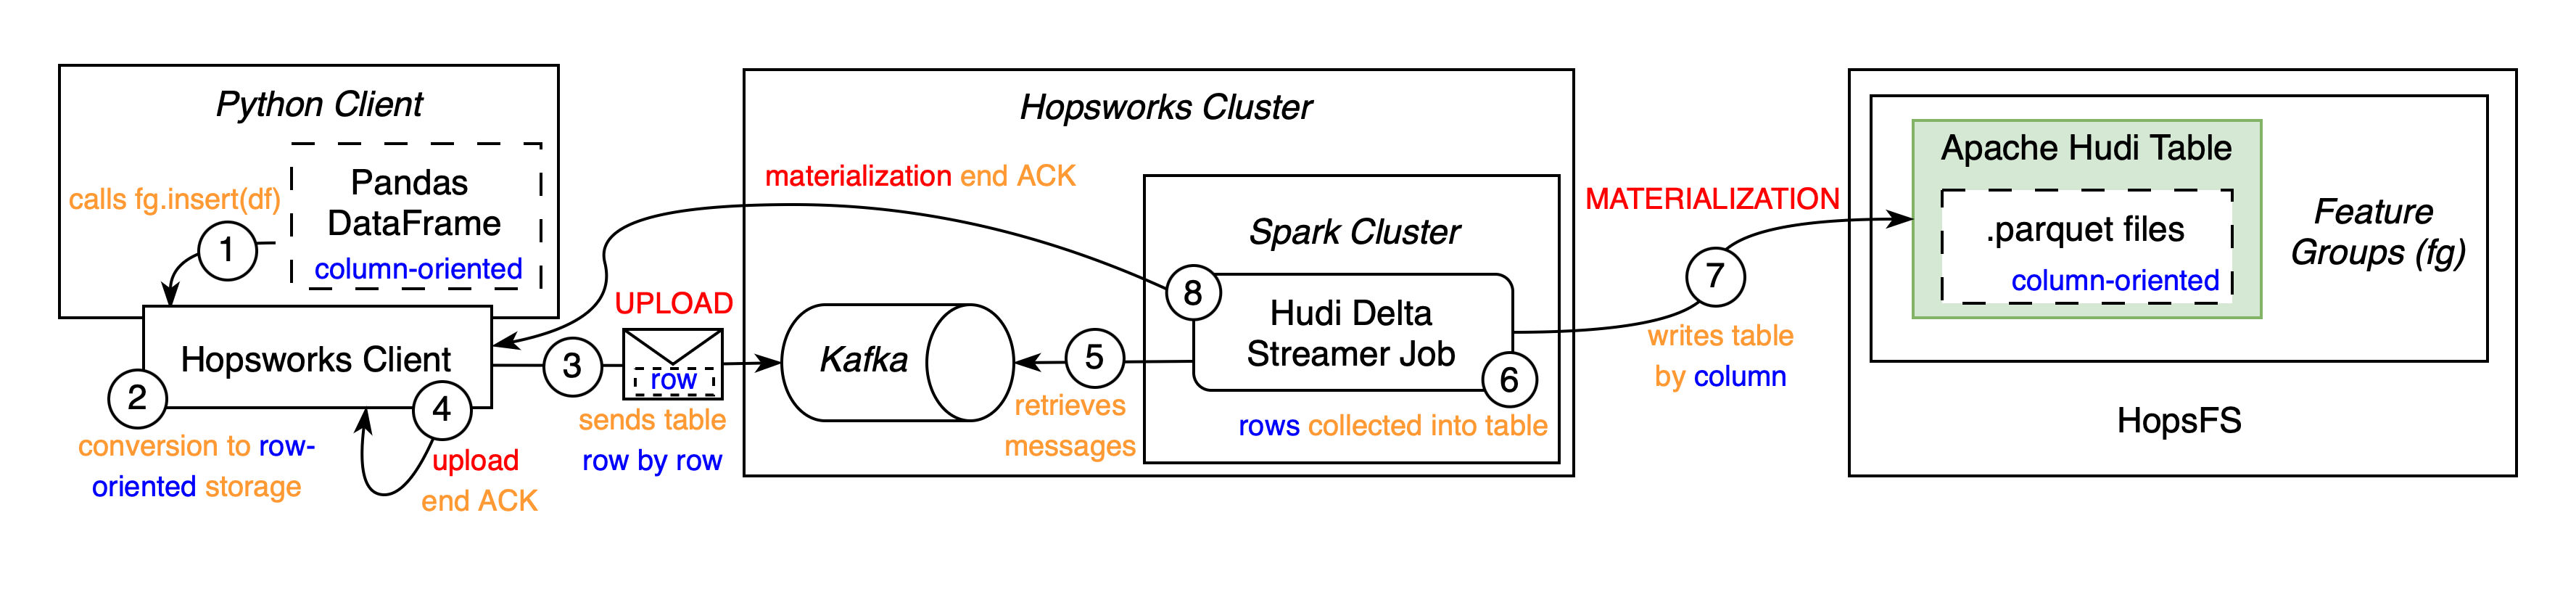
\includegraphics[angle=90,origin=c,keepaspectratio,height=12.5cm]{figures/2-background/FeatureStore-writing.png}
    \end{center}
    \caption[Legacy system - Write process - Magnified diagram]{Legacy system writing a Pandas data frame from a Python client to the Hopsworks offline Feature Store.  This image was magnified to enhance visualization.}
    \label{fig:appx_featurestore_writing}
\end{figure}

\begin{figure}
    \begin{center}
      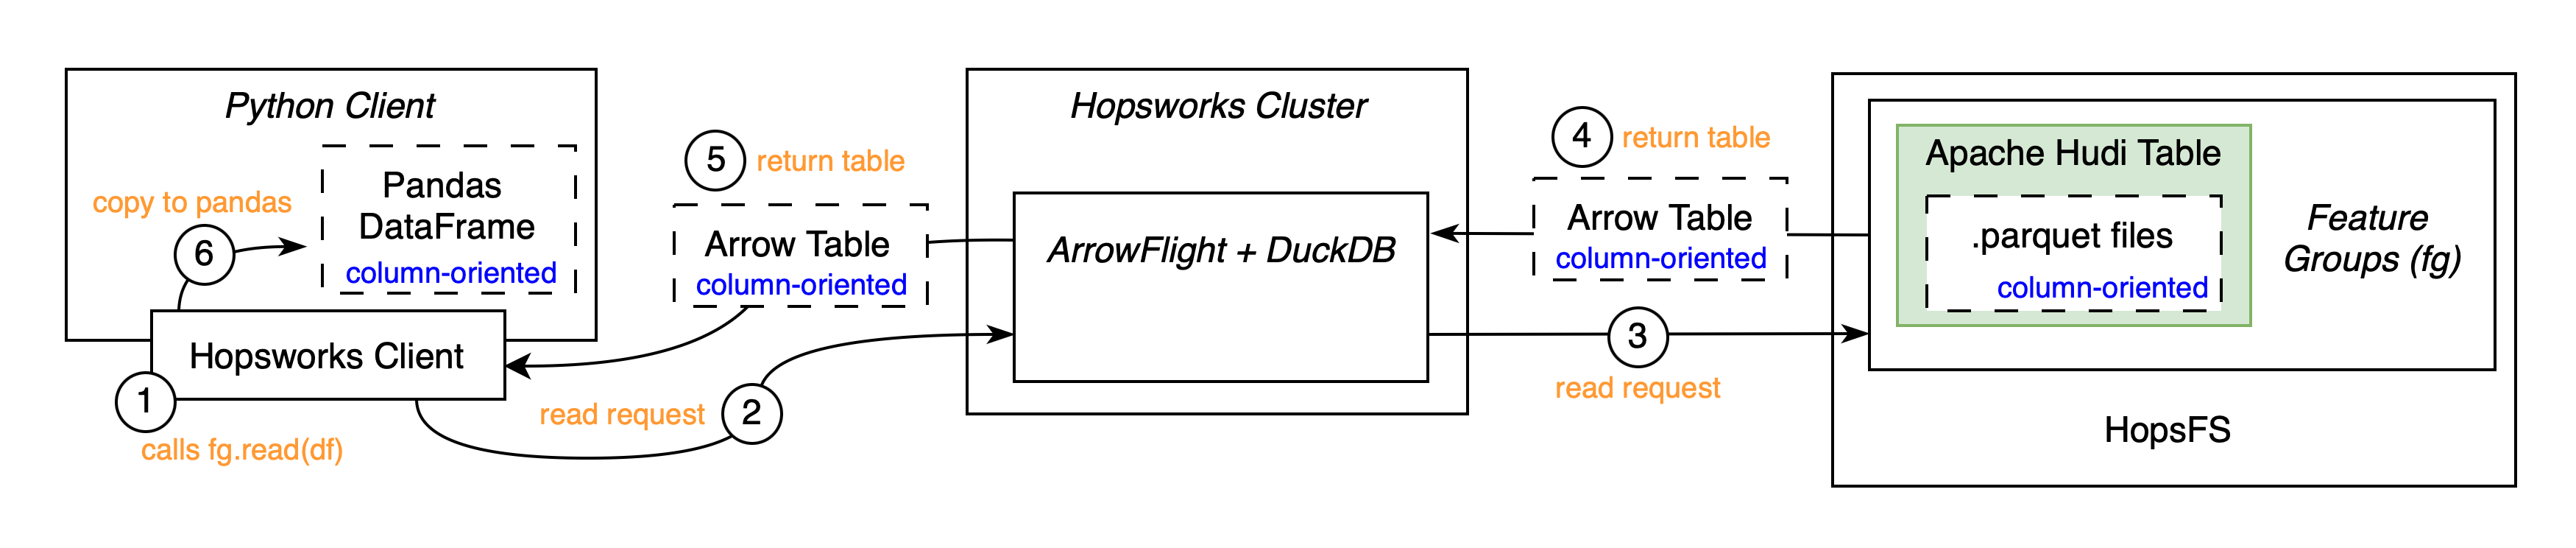
\includegraphics[angle=90,origin=c,keepaspectratio,height=12.5cm]{figures/2-background/FeatureStore-reading.png}
    \end{center}
    \caption[Legacy system - Read process - Magnified diagram]{Legacy system reading a table from the Hopsworks offline feature store and loading it into the Python client local memory. This image was magnified to enhance visualization.}
    \label{fig:appx_featurestore_reading}
\end{figure}

\chapter{Write experiments results}
    \label{appx:res_write}
    % Brief expl
This appendix reports all graphs and tables related to all the writing experiments conducted. Results are reported first expressed as latency (measured during the experiments), then as throughput (computed from the latency and table size).

%%%%%%%%%%%%%%%%%%%%%%%%%%%%%%%%%%%%%%%%%%%%%%%%%%%%%%%%%%%%%%%%%
%%%%%%%%%%%%              LATENCY             %%%%%%%%%%%%%%%%%%%
%%%%%%%%%%%%%%%%%%%%%%%%%%%%%%%%%%%%%%%%%%%%%%%%%%%%%%%%%%%%%%%%%
\begin{figure}
    \centering
    \begin{minipage}[b]{\textwidth}
        \centering
        \captionof{table}[Write experiment - Latency - 1 CPU core]{Write experiment results expressed as latency. The experiment was performed with one \glstext{CPU} core.}
        \label{tbl:appx_res_write_time_1_core}
        \begin{tabular}{c r S[table-format=5.5] S[table-format=5.5] S[table-format=5.5]} 
            \toprule
            \multirow{2}{*}{{Pipeline\Tstrut\Bstrut}} & \multirow{2}{*}{{\thead{Number\\ of rows}}} & {\multirow{2}{*}{{\thead{Latency \\ (seconds)}}}} & \multicolumn{2}{c}{{\thead{Latency (seconds) \\95\% Confidence Interval}}}\\
                                                      &                                             &                                                   & {low} & {high}\\
            \midrule
            \multirow{5}{4em}{delta-rs\\ HopsFS} & 10K  &    1.25088 &    1.23807 &   1.26545\\ 
                                                 & 100K &    1.36828 &    1.33757 &   1.38982\\ 
                                                 & 1M   &    9.38152 &    9.23971 &   9.52904\\
                                                 & 6M   &   19.75469 &   19.33270 &  20.11785\\
                                                 & 60M  &  177.30707 &  174.62871 & 180.01732\\
            \midrule
            \multirow{5}{4em}{delta-rs\\ LocalFS} & 10K  &    0.03957 &   0.03770 &   0.04153\\ 
                                                  & 100K &    0.15240 &   0.14598 &   0.15888\\ 
                                                  & 1M   &    8.42252 &   8.28396 &   8.56376\\
                                                  & 6M   &   17.90634 &  17.48040 &  18.33585\\
                                                  & 60M  &  172.34552 & 169.74808 & 174.73138\\
            \midrule
            \multirow{5}{4em}{Legacy} & 10K  &    50.22767 &   49.53501 &   50.93664\\ 
                                      & 100K &    59.56187 &   58.89466 &   60.18496\\ 
                                      & 1M   &   112.19048 &  111.37162 &  113.00915\\
                                      & 6M   &   511.81693 &  510.75113 &  512.83672\\
                                      & 60M  &  2715.77285 & 2699.88061 & 2731.95225\\
            \bottomrule
        \end{tabular}
    \end{minipage}
    \begin{minipage}[b]{\textwidth}
        \centering
        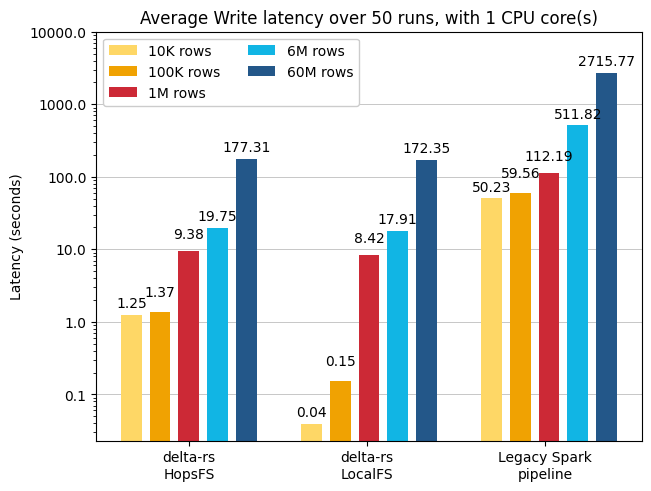
\includegraphics[width=\textwidth]{figures/99-appendix/results-diagrams/write/write_time_1_core.png}
        \caption[Histogram of the write experiment - Latency - 1 CPU core]{Histogram in log-scale of the write experiment results expressed as latency. The experiment was performed with one \glstext{CPU} core.}
        \label{fig:appx_res_write_time_1_core}
    \end{minipage}
\end{figure}

\begin{figure}
    \centering
    \begin{minipage}[b]{\textwidth}
        \centering
        \captionof{table}[Write experiment - Latency - 2 CPU cores]{Write experiment results expressed as latency. The experiment was performed with two \glstext{CPU} cores.}
        \label{tbl:appx_res_write_time_2_cores}
        \begin{tabular}{c r S[table-format=5.5] S[table-format=5.5] S[table-format=5.5]} 
            \toprule
            \multirow{2}{*}{{Pipeline\Tstrut\Bstrut}} & \multirow{2}{*}{{\thead{Number\\ of rows}}} & {\multirow{2}{*}{{\thead{Latency \\ (seconds)}}}} & \multicolumn{2}{c}{{\thead{Latency (seconds) \\95\% Confidence Interval}}}\\
                                                      &                                             &                                                   & {low} & {high}\\
            \midrule
            \multirow{5}{4em}{delta-rs\\ HopsFS} & 10K  &    1.26239 &    1.25079 &   1.27639\\ 
                                                 & 100K &    1.30812 &    1.28050 &   1.33217\\ 
                                                 & 1M   &    8.51536 &    8.34333 &   8.70077\\
                                                 & 6M   &   16.29042 &   15.90659 &  16.67362\\
                                                 & 60M  &  134.06089 &  131.65031 & 136.39761\\
            \midrule
            \multirow{5}{4em}{delta-rs\\ LocalFS} & 10K  &    0.04823 &   0.04640 &   0.04997\\ 
                                                  & 100K &    0.13714 &   0.13402 &   0.14050\\ 
                                                  & 1M   &    7.18530 &   7.03747 &   7.35128\\
                                                  & 6M   &   15.26632 &  14.85172 &  15.65167\\
                                                  & 60M  &  129.82007 & 127.60020 & 132.04689\\
            \midrule
            \multirow{5}{4em}{Legacy} & 10K  &    50.72405 &   50.10769 &   51.30686\\ 
                                      & 100K &    59.78810 &   58.97997 &   60.47427\\ 
                                      & 1M   &   108.56499 &  108.01124 &  109.08128\\
                                      & 6M   &   473.37954 &  472.34534 &  474.43740\\
                                      & 60M  &  2340.77013 & 2333.99443 & 2347.97127\\
            \bottomrule
        \end{tabular}
    \end{minipage}
    \begin{minipage}[b]{\textwidth}
        \centering
        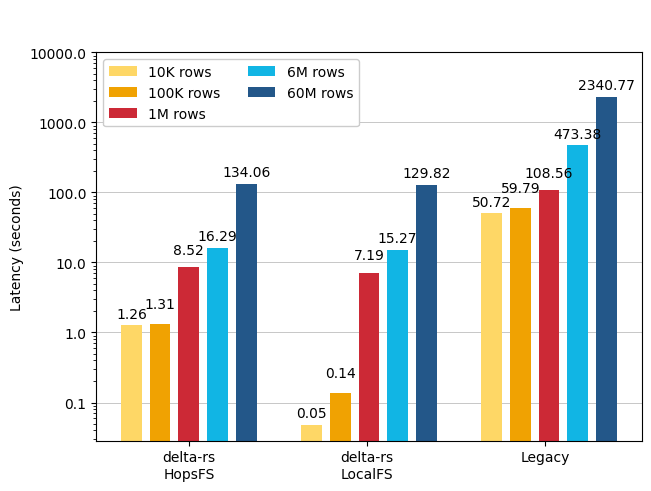
\includegraphics[width=\textwidth]{figures/99-appendix/results-diagrams/write/write_time_2_core.png}
        \caption[Histogram of the write experiment - Latency - 2 CPU cores]{Histogram in log-scale of the write experiment results expressed as latency. The experiment was performed with two \glstext{CPU} cores.}
        \label{fig:appx_res_write_time_2_cores}
    \end{minipage}
\end{figure}

\begin{figure}
    \centering
    \begin{minipage}[b]{\textwidth}
        \centering
        \captionof{table}[Write experiment - Latency - 4 CPU cores]{Write experiment results expressed as latency. The experiment was performed with four \glstext{CPU} cores.}
        \label{tbl:appx_res_write_time_4_cores}
        \begin{tabular}{c r S[table-format=5.5] S[table-format=5.5] S[table-format=5.5]} 
            \toprule
            \multirow{2}{*}{{Pipeline\Tstrut\Bstrut}} & \multirow{2}{*}{{\thead{Number\\ of rows}}} & {\multirow{2}{*}{{\thead{Latency \\ (seconds)}}}} & \multicolumn{2}{c}{{\thead{Latency (seconds) \\95\% Confidence Interval}}}\\
                                                      &                                             &                                                   & {low} & {high}\\
            \midrule
            \multirow{5}{4em}{delta-rs\\ HopsFS} & 10K  &    1.21642 &    1.20232 &   1.23231\\ 
                                                 & 100K &    1.33622 &    1.32294 &   1.34942\\ 
                                                 & 1M   &    8.41325 &    8.24770 &   8.58272\\
                                                 & 6M   &   16.22402 &   15.87946 &  16.59586\\
                                                 & 60M  &  124.10242 &  121.57723 & 126.81530\\
            \midrule
            \multirow{5}{4em}{delta-rs\\ LocalFS} & 10K  &    0.04572 &   0.04341 &   0.04807\\ 
                                                  & 100K &    0.13176 &   0.12880 &   0.13499\\ 
                                                  & 1M   &    7.18574 &   7.00679 &   7.36343\\
                                                  & 6M   &   14.55578 &  14.17679 &  14.94192\\
                                                  & 60M  &  121.37623 & 119.17256 & 123.69890\\
            \midrule
            \multirow{5}{4em}{Legacy} & 10K  &    51.28465 &   50.62282 &   51.90367\\ 
                                      & 100K &    59.52655 &   58.90537 &   60.15322\\ 
                                      & 1M   &   108.81674 &  108.25217 &  109.34234\\
                                      & 6M   &   481.98353 &  481.04435 &  482.92992\\
                                      & 60M  &  2346.04687 & 2336.99396 & 2355.19897\\
            \bottomrule
        \end{tabular}
    \end{minipage}
    \begin{minipage}[b]{\textwidth}
        \centering
        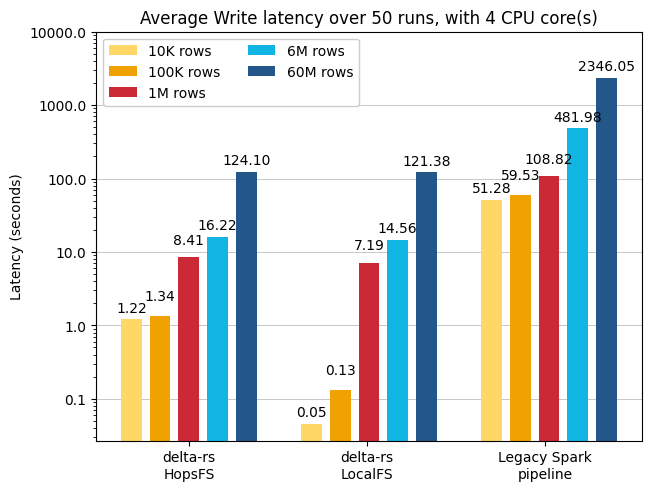
\includegraphics[width=\textwidth]{figures/99-appendix/results-diagrams/write/write_time_4_core.png}
        \caption[Histogram of the write experiment - Latency - 4 CPU cores]{Histogram in log-scale of the write experiment results expressed as latency. The experiment was performed with four \glstext{CPU} cores.}
        \label{fig:appx_res_write_time_4_cores}
    \end{minipage}
\end{figure}

\begin{figure}
    \centering
    \begin{minipage}[b]{\textwidth}
        \centering
        \captionof{table}[Write experiment - Latency - 8 CPU cores]{Write experiment results expressed as latency. The experiment was performed with eight \glstext{CPU} cores.}
        \label{tbl:appx_res_write_time_8_cores}
        \begin{tabular}{c r S[table-format=5.5] S[table-format=5.5] S[table-format=5.5]} 
            \toprule
            \multirow{2}{*}{{Pipeline\Tstrut\Bstrut}} & \multirow{2}{*}{{\thead{Number\\ of rows}}} & {\multirow{2}{*}{{\thead{Latency \\ (seconds)}}}} & \multicolumn{2}{c}{{\thead{Latency (seconds) \\95\% Confidence Interval}}}\\
                                                      &                                             &                                                   & {low} & {high}\\
            \midrule
            \multirow{5}{4em}{delta-rs\\ HopsFS} & 10K  &    1.36756 &    1.24934 &   1.57224\\ 
                                                 & 100K &    1.29243 &    1.26548 &   1.31099\\ 
                                                 & 1M   &    8.30120 &    8.14918 &   8.47040\\
                                                 & 6M   &   15.73847 &   15.28974 &  16.16084\\
                                                 & 60M  &  121.95014 &  119.59376 & 124.18097\\
            \midrule
            \multirow{5}{4em}{delta-rs\\ LocalFS} & 10K  &    0.04402 &   0.04174 &   0.04640\\ 
                                                  & 100K &    0.13648 &   0.13281 &   0.14061\\ 
                                                  & 1M   &    7.22872 &   7.07511 &   7.39893\\
                                                  & 6M   &   14.28157 &  13.90508 &  14.66126\\
                                                  & 60M  &  119.97915 & 117.76416 & 122.20882\\
            \midrule
            \multirow{5}{4em}{Legacy} & 10K  &    51.22859 &   50.59478 &   51.86476\\ 
                                      & 100K &    60.27751 &   59.72907 &   60.77130\\ 
                                      & 1M   &   109.38189 &  108.86830 &  109.88263\\
                                      & 6M   &   475.94345 &  474.83993 &  477.05274\\
                                      & 60M  &  2324.97917 & 2319.04203 & 2331.04794\\
            \bottomrule
        \end{tabular}
    \end{minipage}
    \begin{minipage}[b]{\textwidth}
        \centering
        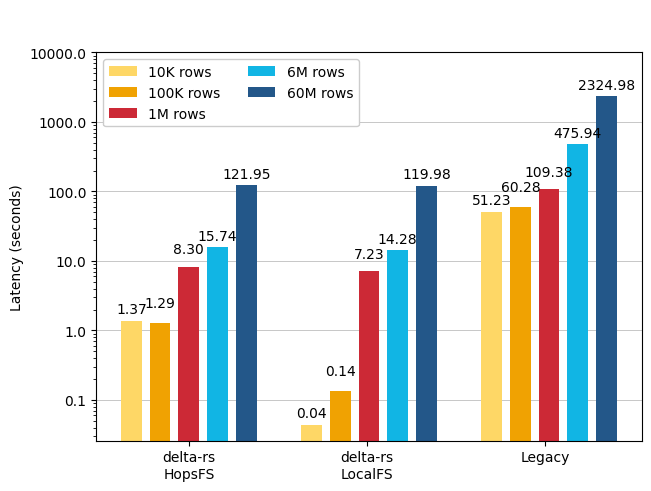
\includegraphics[width=\textwidth]{figures/99-appendix/results-diagrams/write/write_time_8_core.png}
        \caption[Histogram of the write experiment - Latency - 8 CPU cores]{Histogram in log-scale of the write experiment results expressed as latency. The experiment was performed with eight \glstext{CPU} cores.}
        \label{fig:appx_res_write_time_8_cores}
    \end{minipage}
\end{figure}

%%%%%%%%%%%%%%%%%%%%%%%%%%%%%%%%%%%%%%%%%%%%%%%%%%%%%%%%%%%%%%%%%
%%%%%%%%%%%%             THROUGHPUT           %%%%%%%%%%%%%%%%%%%
%%%%%%%%%%%%%%%%%%%%%%%%%%%%%%%%%%%%%%%%%%%%%%%%%%%%%%%%%%%%%%%%%

\begin{figure}
    \centering
    \begin{minipage}[b]{\textwidth}
        \centering
        \captionof{table}[Write experiment - Throughput - 1 CPU core]{Write experiment results expressed as throughput. The experiment was performed with one \glstext{CPU} core.}
        \label{tbl:appx_res_write_throughput_1_core}
        \begin{tabular}{c r S[table-format=5.5] S[table-format=5.5] S[table-format=5.5]} 
            \toprule
            \multirow{2}{*}{{Pipeline\Tstrut\Bstrut}} & \multirow{2}{*}{{\thead{Number\\ of rows}}} & {\multirow{2}{*}{{\thead{Throughput \\ (k rows/second)}}}} & \multicolumn{2}{c}{{\thead{Throughput (k rows/second) \\95\% Confidence Interval}}}\\
                                                      &                                             &                                                          & {low} & {high}\\
            \midrule
            \multirow{5}{4em}{delta-rs\\ HopsFS} & 10K  &    7.99436 &    7.90230 &   8.07705\\ 
                                                 & 100K &    7.30843 &    7.19514 &   7.47621\\ 
                                                 & 1M   &  106.59242 &  104.94226 & 108.22850\\
                                                 & 6M   &  303.72533 &  298.24252 & 310.35491\\
                                                 & 60M  &  338.39598 &  333.30126 & 343.58610\\
            \midrule
            \multirow{5}{4em}{delta-rs\\ LocalFS} & 10K  &  252.68238 &  240.73405 &  265.18632\\ 
                                                  & 100K &  656.15739 &  629.36777 &  684.98518\\ 
                                                  & 1M   &  118.72919 &  116.77110 &  120.71514\\
                                                  & 6M   &  335.07675 &  327.22770 &  343.24143\\
                                                  & 60M  &  348.13784 &  343.38422 &  353.46496\\
            \midrule
            \multirow{5}{4em}{Legacy} & 10K  &     0.19909 &    0.19632 &    0.20187\\ 
                                      & 100K &     1.67892 &    1.66154 &    1.69794\\ 
                                      & 1M   &     8.91341 &    8.84884 &    8.97894\\
                                      & 6M   &    11.72294 &   11.69963 &   11.74740\\
                                      & 60M  &    22.09315 &   21.96231 &   22.22320\\
            \bottomrule
        \end{tabular}
    \end{minipage}
    \begin{minipage}[b]{\textwidth}
        \centering
        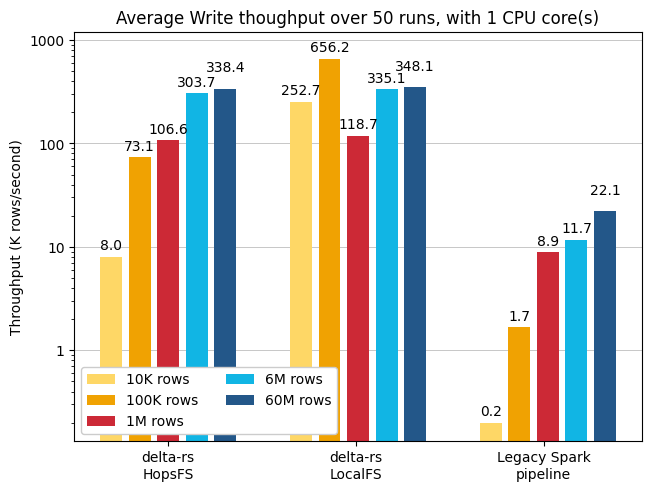
\includegraphics[width=\textwidth]{figures/99-appendix/results-diagrams/write/write_throughput_1_core.png}
        \caption[Histogram of the write experiment - Throughput - 1 CPU core]{Histogram in log-scale of the write experiment results expressed as throughput. The experiment was performed with one \glstext{CPU} core.}
        \label{fig:appx_res_write_throughput_1_core}
    \end{minipage}
\end{figure}

\begin{figure}
    \centering
    \begin{minipage}[b]{\textwidth}
        \centering
        \captionof{table}[Write experiment - Throughput - 2 CPU cores]{Write experiment results expressed as throughput. The experiment was performed with two \glstext{CPU} cores.}
        \label{tbl:appx_res_write_throughput_2_cores}
        \begin{tabular}{c r S[table-format=5.5] S[table-format=5.5] S[table-format=5.5]} 
            \toprule
            \multirow{2}{*}{{Pipeline\Tstrut\Bstrut}} & \multirow{2}{*}{{\thead{Number\\ of rows}}} & {\multirow{2}{*}{{\thead{Throughput \\ (k rows/second)}}}} & \multicolumn{2}{c}{{\thead{Throughput (k rows/second) \\95\% Confidence Interval}}}\\
                                                      &                                             &                                                          & {low} & {high}\\
            \midrule
            \multirow{5}{4em}{delta-rs\\ HopsFS} & 10K  &    7.92146 &    7.83458 &   7.99491\\ 
                                                 & 100K &   76.44507 &   75.06499 &  78.09433\\ 
                                                 & 1M   &  117.43478 &  114.93231 & 119.85614\\
                                                 & 6M   &  368.31440 &  359.84975 & 377.20198\\
                                                 & 60M  &  447.55780 &  439.89038 & 455.75281\\
            \midrule
            \multirow{5}{4em}{delta-rs\\ LocalFS} & 10K  &  207.31922 &  200.08626 &  215.49342\\ 
                                                  & 100K &  729.15967 &  711.73966 &  746.13854\\ 
                                                  & 1M   &  139.17297 &  136.03055 &  142.09647\\
                                                  & 6M   &  393.02185 &  383.34560 &  403.99352\\
                                                  & 60M  &  462.17814 &  454.38403 &  470.21868\\
            \midrule
            \multirow{5}{4em}{Legacy} & 10K  &     0.19714 &    0.19490 &    0.19957\\ 
                                      & 100K &     1.67257 &    1.65359 &    1.69549\\ 
                                      & 1M   &     9.21107 &    9.16747 &    9.25829\\
                                      & 6M   &    12.67481 &   12.64655 &   12.70257\\
                                      & 60M  &    25.63258 &   25.55397 &   25.70700\\
            \bottomrule
        \end{tabular}
    \end{minipage}
    \begin{minipage}[b]{\textwidth}
        \centering
        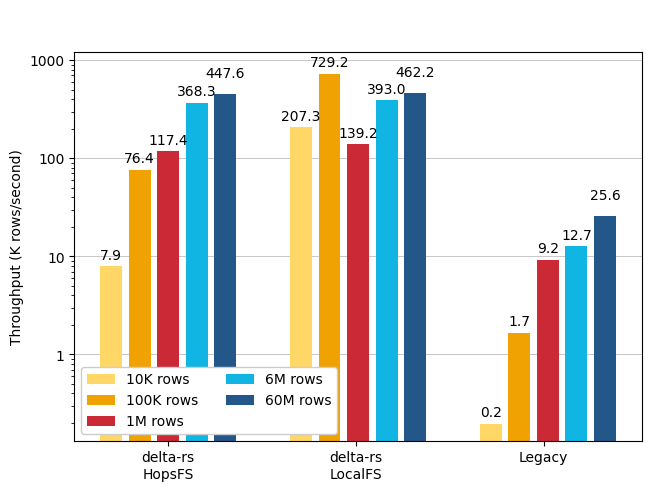
\includegraphics[width=\textwidth]{figures/99-appendix/results-diagrams/write/write_throughput_2_core.png}
        \caption[Histogram of the write experiment - Throughput - 2 CPU cores]{Histogram in log-scale of the write experiment results expressed as throughput. The experiment was performed with two \glstext{CPU} cores.}
        \label{fig:appx_res_write_throughput_2_cores}
    \end{minipage}
\end{figure}

\begin{figure}
    \centering
    \begin{minipage}[b]{\textwidth}
        \centering
        \captionof{table}[Write experiment - Throughput - 4 CPU cores]{Write experiment results expressed as throughput. The experiment was performed with four \glstext{CPU} cores.}
        \label{tbl:appx_res_write_throughput_4_cores}
        \begin{tabular}{c r S[table-format=5.5] S[table-format=5.5] S[table-format=5.5]} 
            \toprule
            \multirow{2}{*}{{Pipeline\Tstrut\Bstrut}} & \multirow{2}{*}{{\thead{Number\\ of rows}}} & {\multirow{2}{*}{{\thead{Throughput \\ (k rows/second)}}}} & \multicolumn{2}{c}{{\thead{Throughput (k rows/second) \\95\% Confidence Interval}}}\\
                                                      &                                             &                                                          & {low} & {high}\\
            \midrule
            \multirow{5}{4em}{delta-rs\\ HopsFS} & 10K  &    8.22083 &    8.11482 &   8.11482\\ 
                                                 & 100K &   74.83742 &   74.10566 &  75.58871\\ 
                                                 & 1M   &  118.86008 &  116.51310 & 121.24582\\
                                                 & 6M   &  369.82202 &  361.53577 & 377.84652\\
                                                 & 60M  &  483.47160 &  473.12899 & 493.51343\\
            \midrule
            \multirow{5}{4em}{delta-rs\\ LocalFS} & 10K  &  218.71364 &  208.02604 &  230.31412\\ 
                                                  & 100K &  758.92422 &  740.79474 &  776.39115\\ 
                                                  & 1M   &  139.16432 &  135.80613 &  142.71864\\
                                                  & 6M   &  412.20728 &  401.55459 &  423.22678\\
                                                  & 60M  &  494.33070 &  485.04875 &  503.47156\\
            \midrule
            \multirow{5}{4em}{Legacy} & 10K  &     0.19499 &    0.19266 &    0.19753\\ 
                                      & 100K &     1.67992 &    1.66242 &    1.69763\\ 
                                      & 1M   &     9.18976 &    9.14558 &    9.23768\\
                                      & 6M   &    12.44855 &   12.42416 &   12.47286\\
                                      & 60M  &    25.57493 &   25.47555 &   25.67400\\
            \bottomrule
        \end{tabular}
    \end{minipage}
    \begin{minipage}[b]{\textwidth}
        \centering
        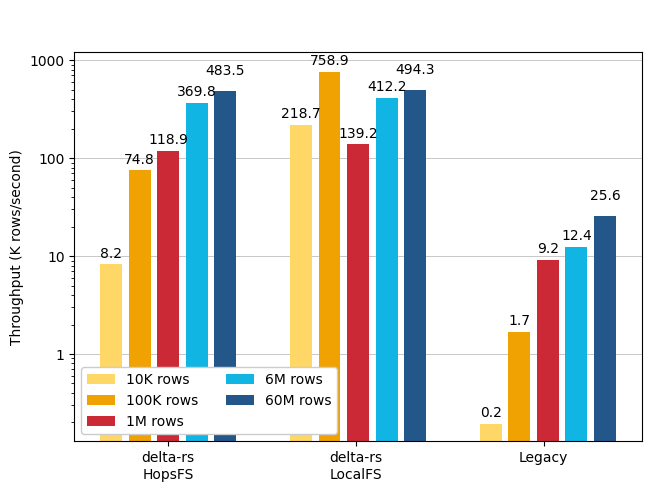
\includegraphics[width=\textwidth]{figures/99-appendix/results-diagrams/write/write_throughput_4_core.png}
        \caption[Histogram of the write experiment - Throughput - 4 CPU cores]{Histogram in log-scale of the write experiment results expressed as throughput. The experiment was performed with four \glstext{CPU} cores.}
        \label{fig:appx_res_write_throughput_4_cores}
    \end{minipage}
\end{figure}

\begin{figure}
    \centering
    \begin{minipage}[b]{\textwidth}
        \centering
        \captionof{table}[Write experiment - Throughput - 8 CPU cores]{Write experiment results expressed as throughput. The experiment was performed with eight \glstext{CPU} cores.}
        \label{tbl:appx_res_write_throughput_8_cores}
        \begin{tabular}{c r S[table-format=5.5] S[table-format=5.5] S[table-format=5.5]} 
            \toprule
            \multirow{2}{*}{{Pipeline\Tstrut\Bstrut}} & \multirow{2}{*}{{\thead{Number\\ of rows}}} & {\multirow{2}{*}{{\thead{Throughput \\ (k rows/second)}}}} & \multicolumn{2}{c}{{\thead{Throughput (k rows/second) \\95\% Confidence Interval}}}\\
                                                      &                                             &                                                          & {low} & {high}\\
            \midrule
            \multirow{5}{4em}{delta-rs\\ HopsFS} & 10K  &    7.31228 &    6.36032 &    8.00422\\ 
                                                 & 100K &   77.37337 &   76.27782 &   79.02104\\ 
                                                 & 1M   &  120.46439 &  118.05814 &  122.71160\\
                                                 & 6M   &  381.23126 &  371.26772 &  392.41978\\
                                                 & 60M  &  492.00431 &  483.16579 &  501.69837\\
            \midrule
            \multirow{5}{4em}{delta-rs\\ LocalFS} & 10K  &  227.12095 &  215.48714 &  239.54128\\ 
                                                  & 100K &  732.70141 &  711.16038 &  752.93200\\ 
                                                  & 1M   &  138.33701 &  135.15466 &  141.34041\\
                                                  & 6M   &  420.12165 &  409.24176 &  431.49669\\
                                                  & 60M  &  500.08688 &  490.96288 &  509.49286\\
            \midrule
            \multirow{5}{4em}{Legacy} & 10K  &     0.19520 &    0.19280 &    0.19764\\ 
                                      & 100K &     1.65899 &    1.64551 &    1.67422\\ 
                                      & 1M   &     9.14228 &    9.10061 &    9.18540\\
                                      & 6M   &    12.60653 &   12.57722 &   12.63583\\
                                      & 60M  &    25.80668 &   25.73949 &   25.87275\\
            \bottomrule
        \end{tabular}
    \end{minipage}
    \begin{minipage}[b]{\textwidth}
        \centering
        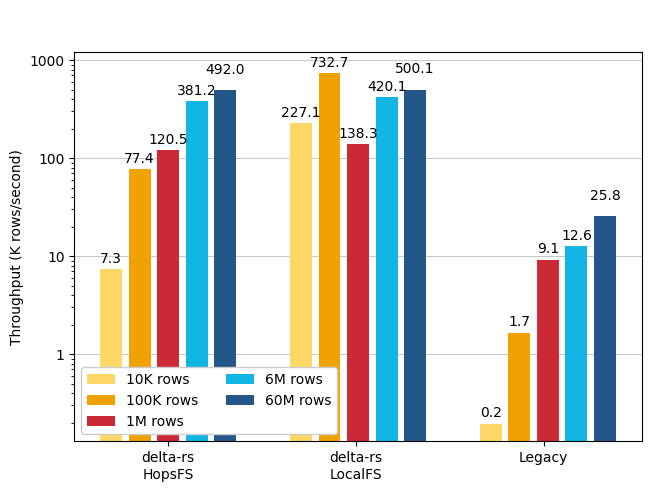
\includegraphics[width=\textwidth]{figures/99-appendix/results-diagrams/write/write_throughput_8_core.png}
        \caption[Histogram of the write experiment - Throughput - 8 CPU cores]{Histogram in log-scale of the write experiment results expressed as throughput. The experiment was performed with eight \glstext{CPU} cores.}
        \label{fig:appx_res_write_throughput_8_cores}
    \end{minipage}
\end{figure}

\chapter{Read experiments results}
    \label{appx:res_read}
    % Brief expl
This appendix reports all graphs and tables related to the read experiments conducted. Results are reported first expressed as latency (measured during the experiments) and then as throughput (computed from the latency and table size).


%%%%%%%%%%%%%%%%%%%%%%%%%%%%%%%%%%%%%%%%%%%%%%%%%%%%%%%%%%%%%%%%%
%%%%%%%%%%%%              LATENCY             %%%%%%%%%%%%%%%%%%%
%%%%%%%%%%%%%%%%%%%%%%%%%%%%%%%%%%%%%%%%%%%%%%%%%%%%%%%%%%%%%%%%%
\begin{figure}
    \centering
    \begin{minipage}[b]{\textwidth}
        \centering
        \captionof{table}[Read experiment - Latency - 1 CPU core]{Read experiment results expressed as latency. The experiment was performed with one \glstext{CPU} core.}
        \label{tbl:appx_res_read_time_1_core}
        \begin{tabular}{c r S[table-format=5.5] S[table-format=5.5] S[table-format=5.5]} 
            \toprule
            \multirow{2}{*}{{Pipeline\Tstrut\Bstrut}} & \multirow{2}{*}{{\thead{Number\\ of rows}}} & {\multirow{2}{*}{{\thead{Latency \\ (seconds)}}}} & \multicolumn{2}{c}{{\thead{Latency (seconds) \\95\% Confidence Interval}}}\\
                                                      &                                             &                                                   & {low} & {high}\\
            \midrule
            \multirow{5}{4em}{delta-rs\\ HopsFS} & 10K  &    0.05342 &    0.03916 &    0.08112\\ 
                                                 & 100K &    0.05757 &    0.05518 &    0.06046\\ 
                                                 & 1M   &    0.53855 &    0.52558 &    0.55229\\
                                                 & 6M   &    1.94899 &    1.93007 &    1.96860\\
                                                 & 60M  &   22.98065 &   22.84067 &   23.14206\\
            \midrule
            \multirow{5}{4em}{delta-rs\\ LocalFS} & 10K  &    0.00419 &    0.00268 &    0.00644\\ 
                                                  & 100K &    0.02696 &    0.01966 &    0.03433\\ 
                                                  & 1M   &    0.42009 &    0.40613 &    0.43563\\
                                                  & 6M   &    1.68223 &    1.65981 &    1.70440\\
                                                  & 60M  &   19.56547 &   19.34690 &   19.77724\\
            \midrule
            \multirow{5}{4em}{Legacy} & 10K  &     0.63159 &    0.62414 &    0.64157\\ 
                                      & 100K &     2.65010 &    2.64272 &    2.65876\\ 
                                      & 1M   &     8.59636 &    8.34094 &    8.90047\\
                                      & 6M   &    33.52964 &   33.23886 &   33.86591\\
                                      & 60M  &    33.69772 &   33.36262 &   34.08665\\
            \bottomrule
        \end{tabular}
    \end{minipage}
    \begin{minipage}[b]{\textwidth}
        \centering
        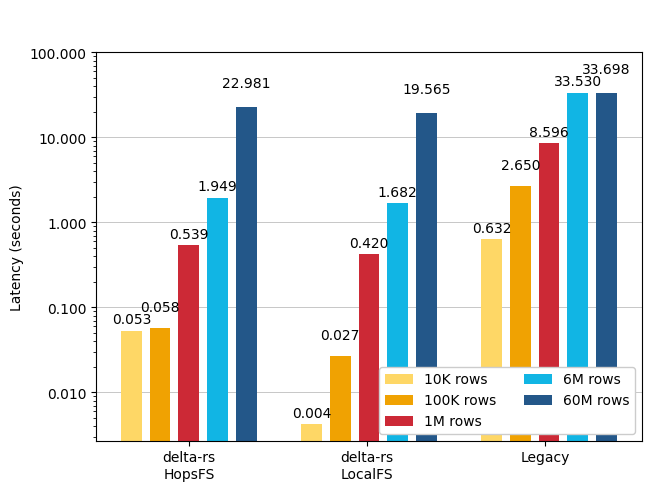
\includegraphics[width=\textwidth]{figures/99-appendix/results-diagrams/read/read_time_1_core.png}
        \caption[Histogram of the read experiment - Latency - 1 CPU core]{Histogram in log-scale of the read experiment results expressed as latency. The experiment was performed with one \glstext{CPU} core.}
        \label{fig:appx_res_read_time_1_core}
    \end{minipage}
\end{figure}

\begin{figure}
    \centering
    \begin{minipage}[b]{\textwidth}
        \centering
        \captionof{table}[Read experiment - Latency - 2 CPU cores]{Read experiment results expressed as latency. The experiment was performed with two \glstext{CPU} cores.}
        \label{tbl:appx_res_read_time_2_cores}
        \begin{tabular}{c r S[table-format=5.5] S[table-format=5.5] S[table-format=5.5]} 
            \toprule
            \multirow{2}{*}{{Pipeline\Tstrut\Bstrut}} & \multirow{2}{*}{{\thead{Number\\ of rows}}} & {\multirow{2}{*}{{\thead{Latency \\ (seconds)}}}} & \multicolumn{2}{c}{{\thead{Latency (seconds) \\95\% Confidence Interval}}}\\
                                                      &                                             &                                                   & {low} & {high}\\
            \midrule
            \multirow{5}{4em}{delta-rs\\ HopsFS} & 10K  &    0.04132 &    0.03933 &    0.04378\\ 
                                                 & 100K &    0.05690 &    0.05123 &    0.06693\\ 
                                                 & 1M   &    0.23413 &    0.22528 &    0.24426\\
                                                 & 6M   &    0.90832 &    0.89967 &    0.91744\\
                                                 & 60M  &   11.41325 &   11.27661 &   11.58899\\
            \midrule
            \multirow{5}{4em}{delta-rs\\ LocalFS} & 10K  &    0.00287 &    0.00278 &    0.00299\\ 
                                                  & 100K &    0.01306 &    0.01041 &    0.01610\\ 
                                                  & 1M   &    0.19977 &    0.18858 &    0.21056\\
                                                  & 6M   &    0.74764 &    0.73503 &    0.76013\\
                                                  & 60M  &    9.44693 &    9.37207 &    9.51753\\
            \midrule
            \multirow{5}{4em}{Legacy} & 10K  &     0.62492 &    0.62210 &    0.62822\\ 
                                      & 100K &     2.66339 &    2.65616 &    2.67166\\ 
                                      & 1M   &     8.61667 &    8.30989 &    8.94938\\
                                      & 6M   &    33.37519 &   33.09688 &   33.67065\\
                                      & 60M  &    33.64281 &   33.30150 &   34.06307\\
            \bottomrule
        \end{tabular}
    \end{minipage}
    \begin{minipage}[b]{\textwidth}
        \centering
        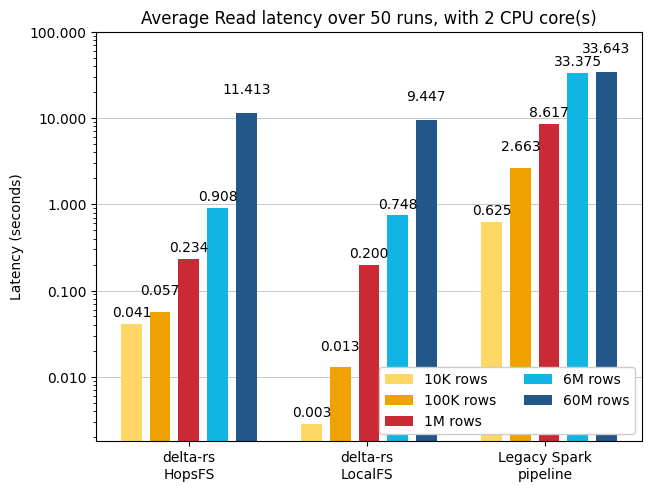
\includegraphics[width=\textwidth]{figures/99-appendix/results-diagrams/read/read_time_2_core.png}
        \caption[Histogram of the read experiment - Latency - 2 CPU cores]{Histogram in log-scale of the read experiment results expressed as latency. The experiment was performed with two \glstext{CPU} cores.}
        \label{fig:appx_res_read_time_2_cores}
    \end{minipage}
\end{figure}

\begin{figure}
    \centering
    \begin{minipage}[b]{\textwidth}
        \centering
        \captionof{table}[Read experiment - Latency - 4 CPU cores]{Read experiment results expressed as latency. The experiment was performed with four \glstext{CPU} cores.}
        \label{tbl:appx_res_read_time_4_cores}
        \begin{tabular}{c r S[table-format=5.5] S[table-format=5.5] S[table-format=5.5]} 
            \toprule
            \multirow{2}{*}{{Pipeline\Tstrut\Bstrut}} & \multirow{2}{*}{{\thead{Number\\ of rows}}} & {\multirow{2}{*}{{\thead{Latency \\ (seconds)}}}} & \multicolumn{2}{c}{{\thead{Latency (seconds) \\95\% Confidence Interval}}}\\
                                                      &                                             &                                                   & {low} & {high}\\
            \midrule
            \multirow{5}{4em}{delta-rs\\ HopsFS} & 10K  &    0.04336 &    0.03922 &   0.05092\\ 
                                                 & 100K &    0.05540 &    0.05378 &   0.05789\\ 
                                                 & 1M   &    0.18847 &    0.15157 &   0.25189\\
                                                 & 6M   &    0.53124 &    0.50778 &   0.57105\\
                                                 & 60M  &    5.58011 &    5.54397 &   5.61936\\
            \midrule
            \multirow{5}{4em}{delta-rs\\ LocalFS} & 10K  &    0.00268 &   0.00259 &   0.00279\\ 
                                                  & 100K &    0.00923 &   0.00852 &   0.01020\\ 
                                                  & 1M   &    0.08971 &   0.08388 &   0.09503\\
                                                  & 6M   &    0.37021 &   0.36018 &   0.38032\\
                                                  & 60M  &    4.81023 &   4.79338 &   4.82789\\
            \midrule
            \multirow{5}{4em}{Legacy} & 10K  &     0.63583 &    0.62352 &    0.65908\\ 
                                      & 100K &     2.63985 &    2.63349 &    2.64623\\ 
                                      & 1M   &     8.75238 &    8.50725 &    9.01383\\
                                      & 6M   &    33.45286 &   33.19461 &   33.75646\\
                                      & 60M  &    33.65245 &   33.27016 &   34.03900\\
            \bottomrule
        \end{tabular}
    \end{minipage}
    \begin{minipage}[b]{\textwidth}
        \centering
        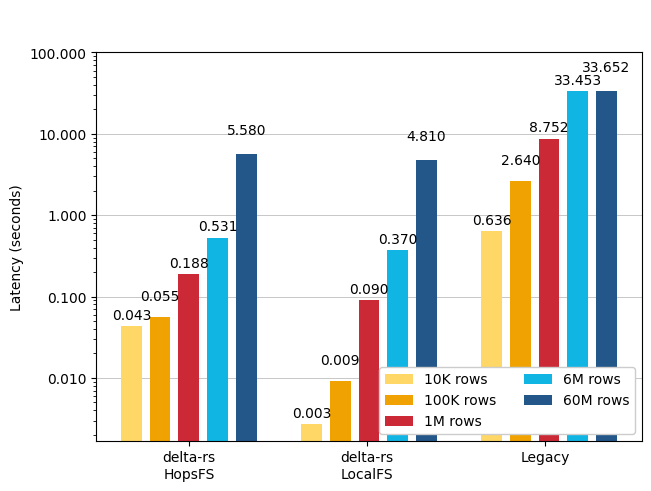
\includegraphics[width=\textwidth]{figures/99-appendix/results-diagrams/read/read_time_4_core.png}
        \caption[Histogram of the read experiment - Latency - 4 CPU cores]{Histogram in log-scale of the read experiment results expressed as latency. The experiment was performed with four \glstext{CPU} cores.}
        \label{fig:appx_res_read_time_4_cores}
    \end{minipage}
\end{figure}

\begin{figure}
    \centering
    \begin{minipage}[b]{\textwidth}
        \centering
        \captionof{table}[Read experiment - Latency - 8 CPU cores]{Read experiment results expressed as latency. The experiment was performed with eight \glstext{CPU} cores.}
        \label{tbl:appx_res_read_time_8_cores}
        \begin{tabular}{c r S[table-format=5.5] S[table-format=5.5] S[table-format=5.5]} 
            \toprule
            \multirow{2}{*}{{Pipeline\Tstrut\Bstrut}} & \multirow{2}{*}{{\thead{Number\\ of rows}}} & {\multirow{2}{*}{{\thead{Latency \\ (seconds)}}}} & \multicolumn{2}{c}{{\thead{Latency (seconds) \\95\% Confidence Interval}}}\\
                                                      &                                             &                                                   & {low} & {high}\\
            \midrule
            \multirow{5}{4em}{delta-rs\\ HopsFS} & 10K  &    0.04330 &    0.03885 &    0.05119\\ 
                                                 & 100K &    0.05458 &    0.05286 &    0.05663\\ 
                                                 & 1M   &    0.17390 &    0.16992 &    0.17808\\
                                                 & 6M   &    0.49729 &    0.48655 &    0.51019\\
                                                 & 60M  &    2.94236 &    2.85554 &    3.06360\\
            \midrule
            \multirow{5}{4em}{delta-rs\\ LocalFS} & 10K  &    0.00294 &    0.00284 &    0.00307\\ 
                                                  & 100K &    0.00948 &    0.00872 &    0.01056\\ 
                                                  & 1M   &    0.04308 &    0.03934 &    0.04830\\
                                                  & 6M   &    0.17548 &    0.17009 &    0.18080\\
                                                  & 60M  &    2.28550 &    2.27501 &    2.29607\\
            \midrule
            \multirow{5}{4em}{Legacy} & 10K  &     0.62739 &    0.62245 &    0.63259\\ 
                                      & 100K &     2.66217 &    2.65309 &    2.67218\\ 
                                      & 1M   &     8.34757 &    8.13471 &    8.60942\\
                                      & 6M   &    33.42815 &   33.15376 &   33.74947\\
                                      & 60M  &    33.14341 &   32.88303 &   33.41299\\
            \bottomrule
        \end{tabular}
    \end{minipage}
    \begin{minipage}[b]{\textwidth}
        \centering
        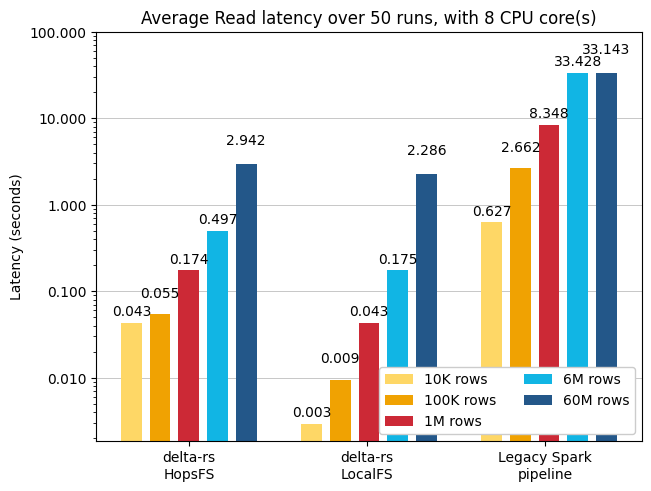
\includegraphics[width=\textwidth]{figures/99-appendix/results-diagrams/read/read_time_8_core.png}
        \caption[Histogram of the read experiment - Latency - 8 CPU cores]{Histogram in log-scale of the read experiment results expressed as latency. The experiment was performed with eight \glstext{CPU} cores.}
        \label{fig:appx_res_read_time_8_cores}
    \end{minipage}
\end{figure}

%%%%%%%%%%%%%%%%%%%%%%%%%%%%%%%%%%%%%%%%%%%%%%%%%%%%%%%%%%%%%%%%%
%%%%%%%%%%%%             THROUGHPUT           %%%%%%%%%%%%%%%%%%%
%%%%%%%%%%%%%%%%%%%%%%%%%%%%%%%%%%%%%%%%%%%%%%%%%%%%%%%%%%%%%%%%%

\begin{figure}
    \centering
    \begin{minipage}[b]{\textwidth}
        \centering
        \captionof{table}[Read experiment - Throughput - 1 CPU core]{Read experiment results expressed as throughput. The experiment was performed with one \glstext{CPU} core.}
        \label{tbl:appx_res_read_throughput_1_core}
        \begin{tabular}{c r S[table-format=5.5] S[table-format=5.5] S[table-format=5.5]} 
            \toprule
            \multirow{2}{*}{{Pipeline\Tstrut\Bstrut}} & \multirow{2}{*}{{\thead{Number\\ of rows}}} & {\multirow{2}{*}{{\thead{Throughput \\ (k rows/second)}}}} & \multicolumn{2}{c}{{\thead{Throughput (k rows/second) \\95\% Confidence Interval}}}\\
                                                      &                                             &                                                          & {low} & {high}\\
            \midrule
            \multirow{5}{4em}{delta-rs\\ HopsFS} & 10K  &  187.16853 &  123.26555 &  255.36173\\ 
                                                 & 100K & 1736.90799 & 1653.91940 & 1811.92857\\ 
                                                 & 1M   & 1856.83167 & 1810.61318 & 1902.65361\\
                                                 & 6M   & 3078.51299 & 3047.83914 & 3108.69431\\
                                                 & 60M  & 2610.89146 & 2592.68185 & 2626.89240\\
            \midrule
            \multirow{5}{4em}{delta-rs\\ LocalFS} & 10K  & 2384.58699 & 1552.08552 & 3721.36068\\ 
                                                  & 100K & 3708.25787 & 2912.43600 & 5084.75715\\ 
                                                  & 1M   & 2380.40381 & 2295.50154 & 2462.25814\\
                                                  & 6M   & 3566.67454 & 3520.29796 & 3614.87006\\
                                                  & 60M  & 3066.62644 & 3033.78996 & 3101.27165\\
            \midrule
            \multirow{5}{4em}{Legacy} & 10K  &    15.83285 &   15.58654 &   16.02196\\ 
                                      & 100K &    37.73432 &   37.61140 &   37.83975\\ 
                                      & 1M   &   116.32820 &  112.35350 &  119.89044\\
                                      & 6M   &   178.94612 &  177.16928 &  180.51159\\
                                      & 60M  &  1780.53563 & 1760.21974 & 1798.41962\\
            \bottomrule
        \end{tabular}
    \end{minipage}
    \begin{minipage}[b]{\textwidth}
        \centering
        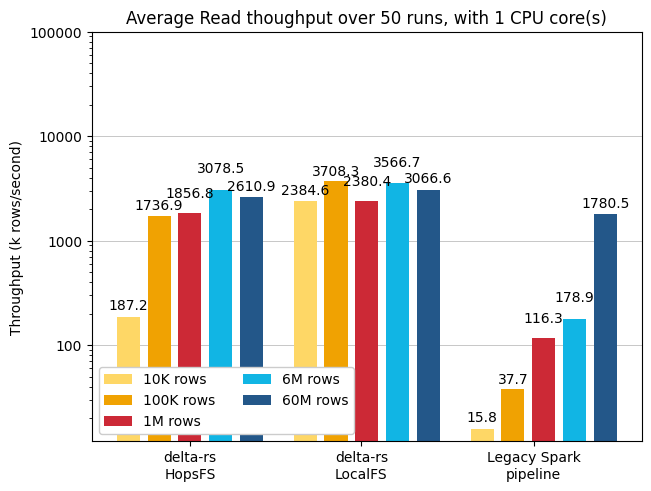
\includegraphics[width=\textwidth]{figures/99-appendix/results-diagrams/read/read_throughput_1_core.png}
        \caption[Histogram of the read experiment - Throughput - 1 CPU core]{Histogram in log-scale of the read experiment results expressed as throughput. The experiment was performed with one \glstext{CPU} core.}
        \label{fig:appx_res_read_throughput_1_core}
    \end{minipage}
\end{figure}

\begin{figure}
    \centering
    \begin{minipage}[b]{\textwidth}
        \centering
        \captionof{table}[Read experiment - Throughput - 2 CPU cores]{Read experiment results expressed as throughput. The experiment was performed with two \glstext{CPU} cores.}
        \label{tbl:appx_res_read_throughput_2_cores}
        \begin{tabular}{c r S[table-format=5.5] S[table-format=5.5] S[table-format=5.5]} 
            \toprule
            \multirow{2}{*}{{Pipeline\Tstrut\Bstrut}} & \multirow{2}{*}{{\thead{Number\\ of rows}}} & {\multirow{2}{*}{{\thead{Throughput \\ (k rows/second)}}}} & \multicolumn{2}{c}{{\thead{Throughput (k rows/second) \\95\% Confidence Interval}}}\\
                                                      &                                             &                                                          & {low} & {high}\\
            \midrule
            \multirow{5}{4em}{delta-rs\\ HopsFS} & 10K  &  241.97833 &  228.37018 &  254.22419\\ 
                                                 & 100K & 1757.17930 & 1494.01876 & 1951.81229\\ 
                                                 & 1M   & 4271.12139 & 4093.98917 & 4438.84612\\
                                                 & 6M   & 6605.54323 & 6539.93631 & 6669.08756\\
                                                 & 60M  & 5257.04658 & 5177.32395 & 5320.74334\\
            \midrule
            \multirow{5}{4em}{delta-rs\\ LocalFS} & 10K  & 3479.95285 & 3339.11982 & 3592.42255\\ 
                                                  & 100K & 7652.74709 & 6210.29638 & 9604.33293\\ 
                                                  & 1M   & 5005.61642 & 4749.17943 & 5302.53656\\
                                                  & 6M   & 8025.19634 & 7893.33251 & 8162.84493\\
                                                  & 60M  & 6351.26715 & 6304.15538 & 6401.99467\\
            \midrule
            \multirow{5}{4em}{Legacy} & 10K  &   16.00183 &   15.91773 &   16.07453\\ 
                                      & 100K &   37.54607 &   37.42979 &   37.64822\\ 
                                      & 1M   &  116.05404 &  111.73951 &  120.33848\\
                                      & 6M   &  179.77424 &  178.19671 &  181.28593\\
                                      & 60M  & 1783.44198 & 1761.43830 & 1801.72013\\
            \bottomrule
        \end{tabular}
    \end{minipage}
    \begin{minipage}[b]{\textwidth}
        \centering
        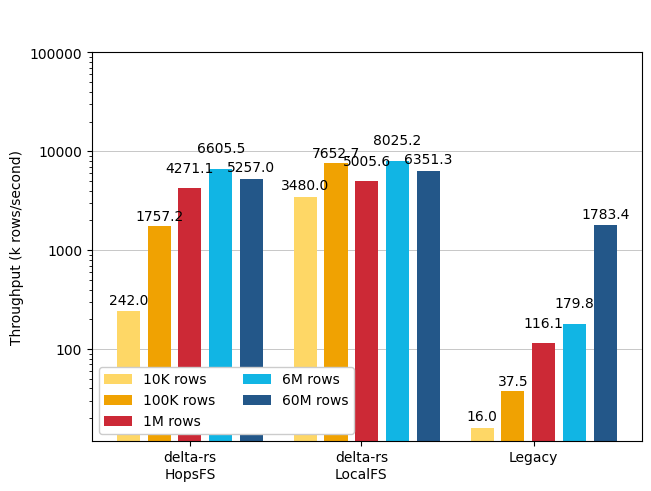
\includegraphics[width=\textwidth]{figures/99-appendix/results-diagrams/read/read_throughput_2_core.png}
        \caption[Histogram of the read experiment - Throughput - 2 CPU cores]{Histogram in log-scale of the read experiment results expressed as throughput. The experiment was performed with two \glstext{CPU} cores.}
        \label{fig:appx_res_read_throughput_2_cores}
    \end{minipage}
\end{figure}

\begin{figure}
    \centering
    \begin{minipage}[b]{\textwidth}
        \centering
        \captionof{table}[Read experiment - Throughput - 4 CPU cores]{Read experiment results expressed as throughput. The experiment was performed with four \glstext{CPU} cores.}
        \label{tbl:appx_res_read_throughput_4_cores}
        \begin{tabular}{c r S[table-format=5.5] S[table-format=5.5] S[table-format=5.5]} 
            \toprule
            \multirow{2}{*}{{Pipeline\Tstrut\Bstrut}} & \multirow{2}{*}{{\thead{Number\\ of rows}}} & {\multirow{2}{*}{{\thead{Throughput \\ (k rows/second)}}}} & \multicolumn{2}{c}{{\thead{Throughput (k rows/second) \\95\% Confidence Interval}}}\\
                                                      &                                             &                                                          & {low} & {high}\\
            \midrule
            \multirow{5}{4em}{delta-rs\\ HopsFS} & 10K  &   230.61925 &   196.37366 &   254.93232\\ 
                                                 & 100K &  1804.73106 &  1727.27256 &  1859.40719\\ 
                                                 & 1M   &  5305.74239 &  3969.95699 &  6597.37404\\
                                                 & 6M   & 11294.12619 & 10506.91939 & 11816.03313\\
                                                 & 60M  & 10752.47511 & 10677.35647 & 10822.55620\\
            \midrule
            \multirow{5}{4em}{delta-rs\\ LocalFS} & 10K  &  3720.94104 &  3572.45085 &  3854.74973\\ 
                                                  & 100K & 10830.88457 &  9802.96062 & 11735.92863\\ 
                                                  & 1M   & 11146.06743 & 10522.54071 & 11921.62257\\
                                                  & 6M   & 16206.97330 & 15775.94387 & 16657.93725\\
                                                  & 60M  & 12473.40492 & 12427.78728 & 12517.25967\\
            \midrule
            \multirow{5}{4em}{Legacy} & 10K  &    15.72724 &   15.17259 &   16.03790\\ 
                                      & 100K &    37.88093 &   37.78959 &   37.97237\\ 
                                      & 1M   &   114.25460 &  110.94061 &  117.54671\\
                                      & 6M   &   179.35680 &  177.74372 &  180.75222\\
                                      & 60M  &  1782.93073 & 1762.68396 & 1803.41764\\
            \bottomrule
        \end{tabular}
    \end{minipage}
    \begin{minipage}[b]{\textwidth}
        \centering
        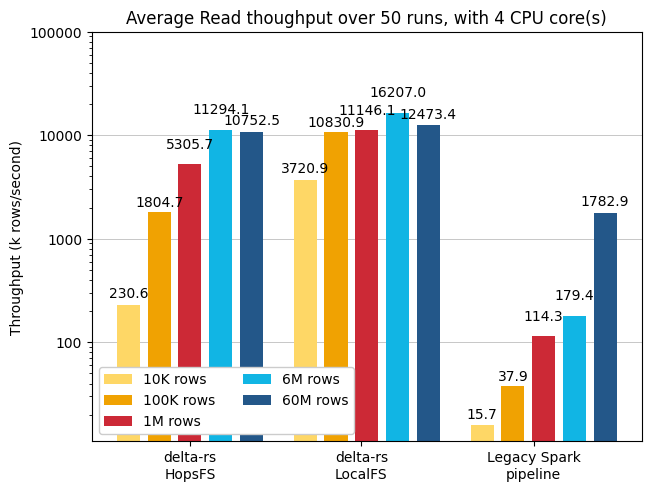
\includegraphics[width=\textwidth]{figures/99-appendix/results-diagrams/read/read_throughput_4_core.png}
        \caption[Histogram of the read experiment - Throughput - 4 CPU cores]{Histogram in log-scale of the read experiment results expressed as throughput. The experiment was performed with four \glstext{CPU} cores.}
        \label{fig:appx_res_read_throughput_4_cores}
    \end{minipage}
\end{figure}

\begin{figure}
    \centering
    \begin{minipage}[b]{\textwidth}
        \centering
        \captionof{table}[Read experiment - Throughput - 8 CPU cores]{Read experiment results expressed as throughput. The experiment was performed with eight \glstext{CPU} cores.}
        \label{tbl:appx_res_read_throughput_8_cores}
        \begin{tabular}{c r S[table-format=5.5] S[table-format=5.5] S[table-format=5.5]} 
            \toprule
            \multirow{2}{*}{{Pipeline\Tstrut\Bstrut}} & \multirow{2}{*}{{\thead{Number\\ of rows}}} & {\multirow{2}{*}{{\thead{Throughput \\ (k rows/second)}}}} & \multicolumn{2}{c}{{\thead{Throughput (k rows/second) \\95\% Confidence Interval}}}\\
                                                      &                                             &                                                          & {low} & {high}\\
            \midrule
            \multirow{5}{4em}{delta-rs\\ HopsFS} & 10K  &   230.92518 &   195.34544 &   257.36067\\ 
                                                 & 100K &  1832.05683 &  1765.75684 &  1891.54456\\ 
                                                 & 1M   &  5750.34366 &  5615.17071 &  5885.01795\\
                                                 & 6M   & 12065.18202 & 11760.17893 & 12331.70977\\
                                                 & 60M  & 20391.77956 & 19584.75363 & 21011.72136\\
            \midrule
            \multirow{5}{4em}{delta-rs\\ LocalFS} & 10K  &  3390.32242 &  3256.07486 &  3510.69231\\ 
                                                  & 100K & 10545.41087 &  9465.27536 & 11463.06073\\ 
                                                  & 1M   & 23212.46679 & 20701.23033 & 25414.13122\\
                                                  & 6M   & 34191.39637 & 33185.18129 & 35275.25456\\
                                                  & 60M  & 26252.42019 & 26131.51836 & 26373.48880\\
            \midrule
            \multirow{5}{4em}{Legacy} & 10K  &    15.93901 &   15.80791 &   16.06539\\ 
                                      & 100K &    37.56330 &   37.42250 &   37.69186\\ 
                                      & 1M   &   119.79520 &  116.15177 &  122.92995\\
                                      & 6M   &   179.48942 &  177.78054 &  180.97490\\
                                      & 60M  &  1810.31436 & 1795.70867 & 1824.64883\\
            \bottomrule
        \end{tabular}
    \end{minipage}
    \begin{minipage}[b]{\textwidth}
        \centering
        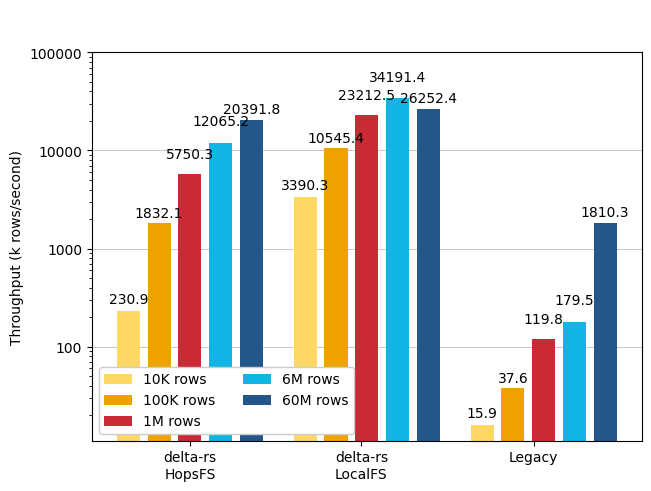
\includegraphics[width=\textwidth]{figures/99-appendix/results-diagrams/read/read_throughput_8_core.png}
        \caption[Histogram of the read experiment - Throughput - 8 CPU cores]{Histogram in log-scale of the read experiment results expressed as throughput. The experiment was performed with eight \glstext{CPU} cores.}
        \label{fig:appx_res_read_throughput_8_cores}
    \end{minipage}
\end{figure}

\chapter{Legacy pipeline write latency breakdown results}
    \label{appx:res_hudi}
    % Brief expl
This appendix reports all graphs and tables related to all write latency breakdown of the upload and materialization steps in the legacy pipeline.

\begin{figure}
    \centering
    \begin{minipage}[b]{\textwidth}
        \centering
        \captionof{table}[Write on legacy pipeline - Time breakdown - 1 core]{Contributions to the write latency of the upload and materialization steps in the legacy pipeline. The experiment was performed with one \glstext{CPU} core.}
        \label{tbl:appx_hudi_virtualiz_breakdown_1_core}
        \begin{tabular}{l r S[table-format=5.4] S[table-format=5.4] S[table-format=5.4] S[table-format=5.4]} 
            \toprule
            {\multirow{2}{*}{Step\Tstrut\Bstrut}} & \multirow{2}{*}{{\thead{Number\\ of rows}}} & {\multirow{2}{*}{{\thead{Latency \\ (seconds)}}}} & \multicolumn{2}{c}{{\thead{Latency (seconds) \\95\% Confidence Interval}}}\\
                                    &                                             &                                                   & {low} & {high}                                                            \\
            \midrule
            upload                  & \multirow{2}{*}{10K}                        &    2.4865                                         &    2.3896 &    2.6261                                                      \\ 
            materialize           &                                             &   47.7262                                         &   47.0445 &   48.4031                                                      \\
            \midrule
            upload                  & \multirow{2}{*}{100K}                       &    3.6684                                         &    3.6310 &    3.7098                                                      \\                                                                 
            materialize            &                                             &   55.9005                                         &   55.2494 &   56.5541                                                      \\
            \midrule
            upload                  & \multirow{2}{*}{1M}                         &   22.5934                                         &   22.4496 &   22.7349                                                      \\                                                                 
            materialize             &                                             &   89.5754                                         &   88.8286 &   90.3049                                                      \\
            \midrule
            upload                 & \multirow{2}{*}{6M}                         &  244.6123                                         &  244.0368 &  245.1905                                                      \\                                                                 
            materialize             &                                             &  267.2490                                         &  266.4287 &  268.1549                                                      \\
            \midrule
            upload                  & \multirow{2}{*}{60M}                         & 2437.7840                                         & 2422.8704 & 2453.6746                                                      \\                                                                 
            materialize             &                                             &  278.0504                                         &  276.2340 &  280.0921                                                      \\
            \bottomrule
        \end{tabular}
    \end{minipage}
    \begin{minipage}[b]{\textwidth}
        \centering
        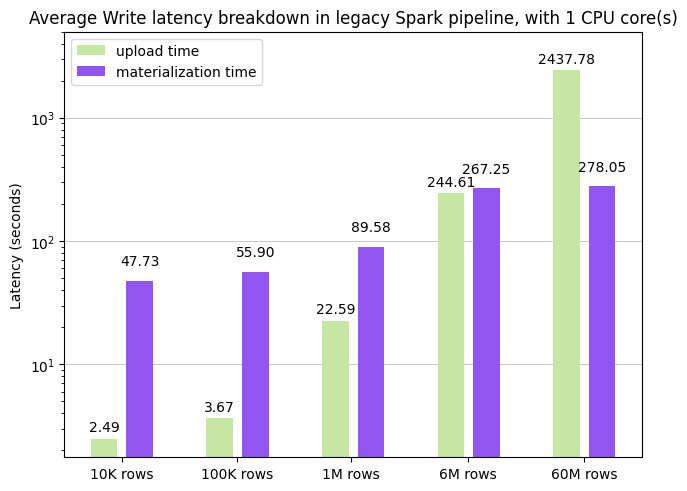
\includegraphics[width=\textwidth]{figures/99-appendix/results-diagrams/write/hudi_upload_materialize/hudi_virtualiz_1_core.png}
        \caption[Histogram of the write on legacy pipeline - Time breakdown - 1 CPU core]{Histogram in log-scale displaying the contributions to the write latency of the upload and materialization steps in the legacy pipeline. The experiment was performed with one \glstext{CPU} core.}
        \label{fig:appx_hudi_virtualiz_breakdown_1_core}
    \end{minipage}
\end{figure}

\begin{figure}
    \centering
    \begin{minipage}[b]{\textwidth}
        \centering
        \captionof{table}[Write on legacy pipeline - Time breakdown - 2 cores]{Contributions to the write latency of the upload and materialization steps in the legacy pipeline. The experiment was performed with two \glstext{CPU} cores.}
        \label{tbl:appx_hudi_virtualiz_breakdown_2_cores}
        \begin{tabular}{l r S[table-format=5.4] S[table-format=5.4] S[table-format=5.4] S[table-format=5.4]} 
            \toprule
            {\multirow{2}{*}{Step\Tstrut\Bstrut}} & \multirow{2}{*}{{\thead{Number\\ of rows}}} & {\multirow{2}{*}{{\thead{Latency \\ (seconds)}}}} & \multicolumn{2}{c}{{\thead{Latency (seconds) \\95\% Confidence Interval}}}\\
                                    &                                             &                                                   & {low} & {high}                                                            \\
            \midrule
            upload                  & \multirow{2}{*}{10K}                        &    2.3873                                         &    2.3276 &    2.4466                                                      \\ 
            materialize             &                                             &   48.3305                                         &   47.7020 &   48.9923                                                      \\
            \midrule
            upload                  & \multirow{2}{*}{100K}                       &    3.4348                                         &    3.4008 &    3.4671                                                      \\                                                                 
            materialize             &                                             &   56.3367                                         &   55.5626 &   57.1129                                                      \\
            \midrule
            upload                  & \multirow{2}{*}{1M}                         &   18.6349                                         &   18.5673 &   18.7104                                                      \\                                                                 
            materialize             &                                             &   89.9267                                         &   89.4012 &   90.4514                                                      \\
            \midrule
            upload                  & \multirow{2}{*}{6M}                         &  205.8854                                         &  205.2177 &  206.4984                                                      \\                                                                 
            materialize             &                                             &  267.5079                                         &  266.6853 &  268.3512                                                      \\
            \midrule
            upload                  & \multirow{2}{*}{60M}                         & 2064.1357                                         & 2057.6396 & 2070.4450                                                      \\                                                                 
            materialize             &                                             &  276.9608                                         &  275.7156 &  278.2849                                                      \\
            \bottomrule
        \end{tabular}
    \end{minipage}
    \begin{minipage}[b]{\textwidth}
        \centering
        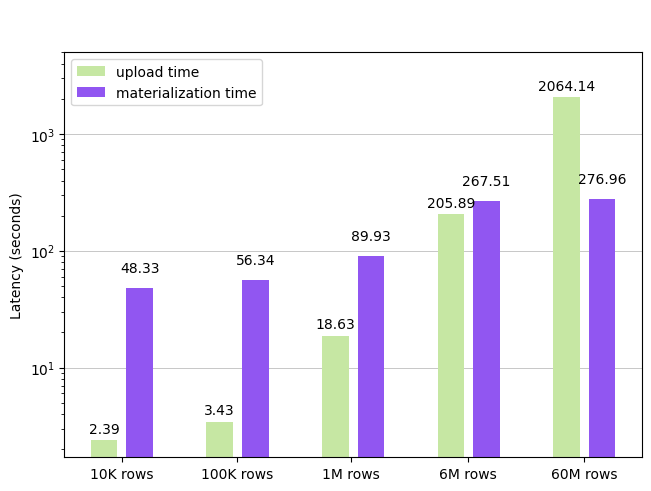
\includegraphics[width=\textwidth]{figures/99-appendix/results-diagrams/write/hudi_upload_materialize/hudi_virtualiz_2_core.png}
        \caption[Histogram of the write on legacy pipeline - Time breakdown - 2 CPU cores]{Histogram in log-scale displaying the contributions to the write latency of the upload and materialization steps in the legacy pipeline. The experiment was performed with two \glstext{CPU} cores.}
        \label{fig:appx_hudi_virtualiz_breakdown_2_core}
    \end{minipage}
\end{figure}

\begin{figure}
    \centering
    \begin{minipage}[b]{\textwidth}
        \centering
        \captionof{table}[Write on legacy pipeline - Time breakdown - 4 cores]{Contributions to the write latency of the upload and materialization steps in the legacy pipeline. The experiment was performed with four \glstext{CPU} cores.}
        \label{tbl:appx_hudi_virtualiz_breakdown_4_cores}
        \begin{tabular}{l r S[table-format=5.4] S[table-format=5.4] S[table-format=5.4] S[table-format=5.4]} 
            \toprule
            {\multirow{2}{*}{Step\Tstrut\Bstrut}} & \multirow{2}{*}{{\thead{Number\\ of rows}}} & {\multirow{2}{*}{{\thead{Latency \\ (seconds)}}}} & \multicolumn{2}{c}{{\thead{Latency (seconds) \\95\% Confidence Interval}}}\\
                                    &                                             &                                                   & {low} & {high}                                                            \\
            \midrule
            upload                  & \multirow{2}{*}{10K}                        &    2.3846                                         &    2.3299 &    2.4335                                                      \\ 
            materialize             &                                             &   48.9061                                         &   48.2436 &   49.5470                                                      \\
            \midrule
            upload                  & \multirow{2}{*}{100K}                       &    3.4650                                         &    3.4245 &    3.5071                                                      \\                                                                 
            materialize             &                                             &   56.0524                                         &   55.3682 &   56.6822                                                      \\
            \midrule
            upload                  & \multirow{2}{*}{1M}                         &   19.2296                                         &   19.1455 &   19.3161                                                      \\                                                                 
            materialize             &                                             &   89.5864                                         &   89.0209 &   90.1313                                                      \\
            \midrule
            upload                  & \multirow{2}{*}{6M}                         &  211.6758                                         &  211.0694 &  212.2839                                                      \\                                                                 
            materialize             &                                             &  270.3233                                         &  269.5967 &  270.9895                                                      \\
            \midrule
            upload                  & \multirow{2}{*}{60M}                         & 2068.5260                                         & 2060.3358 & 2077.2837                                                      \\                                                                 
            materialize             &                                             &  277.6001                                         &  276.0065 &  279.1456                                                      \\
            \bottomrule
        \end{tabular}
    \end{minipage}
    \begin{minipage}[b]{\textwidth}
        \centering
        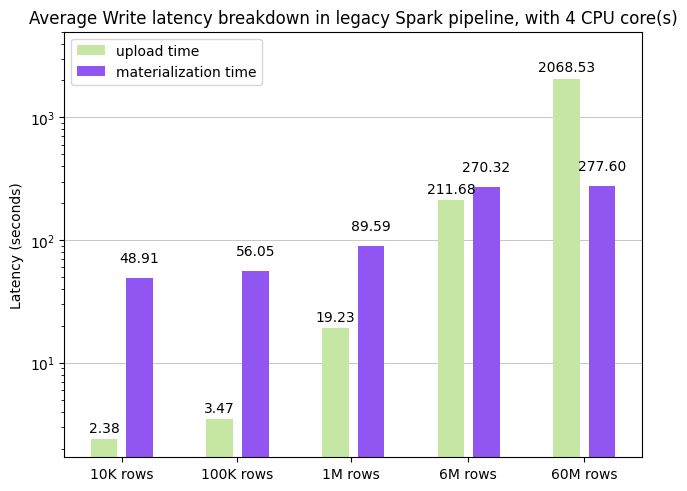
\includegraphics[width=\textwidth]{figures/99-appendix/results-diagrams/write/hudi_upload_materialize/hudi_virtualiz_4_core.png}
        \caption[Histogram of the write on legacy pipeline - Time breakdown - 4 CPU cores]{Histogram in log-scale displaying the contributions to the write latency of the upload and materialization steps in the legacy pipeline. The experiment was performed with four \glstext{CPU} cores.}
        \label{fig:appx_hudi_virtualiz_breakdown_4_core}
    \end{minipage}
\end{figure}

\begin{figure}
    \centering
    \begin{minipage}[b]{\textwidth}
        \centering
        \captionof{table}[Write on legacy pipeline - Time breakdown - 8 cores]{Contributions to the write latency of the upload and materialization steps in the legacy pipeline. The experiment was performed with eight \glstext{CPU} cores.}
        \label{tbl:appx_hudi_virtualiz_breakdown_8_cores}
        \begin{tabular}{l r S[table-format=5.4] S[table-format=5.4] S[table-format=5.4] S[table-format=5.4]} 
            \toprule
            {\multirow{2}{*}{Step\Tstrut\Bstrut}} & \multirow{2}{*}{{\thead{Number\\ of rows}}} & {\multirow{2}{*}{{\thead{Latency \\ (seconds)}}}} & \multicolumn{2}{c}{{\thead{Latency (seconds) \\95\% Confidence Interval}}}\\
                                    &                                             &                                                   & {low} & {high}                                                            \\
            \midrule
            upload                  & \multirow{2}{*}{10K}                        &    2.3815                                         &    2.3304 &    2.4358                                                      \\ 
            materialize             &                                             &   48.8485                                         &   48.1979 &   49.4467                                                      \\
            \midrule
            upload                  & \multirow{2}{*}{100K}                       &    3.4392                                         &    3.4081 &    3.4700                                                      \\                                                                 
            materialize             &                                             &   56.8428                                         &   56.3177 &   57.3685                                                      \\
            \midrule
            upload                  & \multirow{2}{*}{1M}                         &   18.8642                                         &   18.7808 &   18.9532                                                      \\                                                                 
            materialize             &                                             &   90.5153                                         &   90.0306 &   90.9718                                                      \\
            \midrule
            upload                  & \multirow{2}{*}{6M}                         &  207.6646                                         &  207.1606 &  208.2090                                                      \\                                                                 
            materialize             &                                             &  268.2752                                         &  267.3569 &  269.2456                                                      \\
            \midrule
            upload                  & \multirow{2}{*}{60M}                         & 2049.1371                                         & 2043.5991 & 2055.4782                                                      \\                                                                 
            materialize             &                                             &  275.7636                                         &  274.2773 &  274.2773                                                      \\
            \bottomrule
        \end{tabular}
    \end{minipage}
    \begin{minipage}[b]{\textwidth}
        \centering
        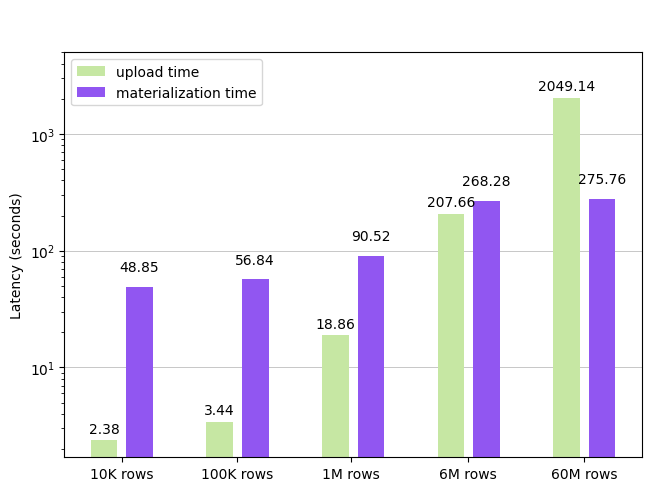
\includegraphics[width=\textwidth]{figures/99-appendix/results-diagrams/write/hudi_upload_materialize/hudi_virtualiz_8_core.png}
        \caption[Histogram of the write on legacy pipeline - Time breakdown - 8 CPU cores]{Histogram in log-scale displaying the contributions to the write latency of the upload and materialization steps in the legacy pipeline. The experiment was performed with eight \glstext{CPU} cores.}
        \label{fig:appx_hudi_virtualiz_breakdown_8_core}
    \end{minipage}
\end{figure}

\cleardoublepage

%% The following label is necessary for computing the last page number of the body of the report to include in the "For DIVA" information
\label{pg:lastPageofMainmatter}

\cleardoublepage
\begin{comment}
%%%%%%%%%%%%%%%%%%%%%%%%%%%%%%%%%%%%%%%%%%%%%%%%%%%%%%%%%%%%%%%%%%%%%%%%%%%%%%%%%%%%%%%%
%%                                 FOR DIVA MATERIAL
%%%%%%%%%%%%%%%%%%%%%%%%%%%%%%%%%%%%%%%%%%%%%%%%%%%%%%%%%%%%%%%%%%%%%%%%%%%%%%%%%%%%%%%%
\clearpage\thispagestyle{empty}\mbox{} % empty page with backcover on the other side
\kthbackcover
\fancyhead{}  % Do not use header on this extra page or pages
\section*{€€€€ For DIVA €€€€}
\lstset{numbers=none} %% remove any list line numbering
\divainfo{pg:lastPageofPreface}{pg:lastPageofMainmatter}

% If there is an acronyms.tex file,
% add it to the end of the For DIVA information
% so that it can be used with the abstracts
% Note that the option "nolol" stops it from being listed in the List of Listings

% The following bit of ugliness is because of the problems PDFLaTeX has handling a non-breaking hyphen
% unless it is converted to UTF-8 encoding.
% If you do not use such characters in your acronyms, this could be simplified.
\ifxeorlua
\IfFileExists{lib/acronyms.tex}{
\section*{acronyms.tex}
\lstinputlisting[language={[LaTeX]TeX}, nolol, basicstyle=\ttfamily\color{black},
commentstyle=\color{black}, backgroundcolor=\color{white}]{lib/acronyms.tex}
}
{}
\else
\IfFileExists{lib/acronyms-for-pdflatex.tex}{
\section*{acronyms.tex}
\lstinputlisting[language={[LaTeX]TeX}, nolol, basicstyle=\ttfamily\color{black},
commentstyle=\color{black}, backgroundcolor=\color{white}]{lib/acronyms-for-pdflatex.tex}
}
{}
\fi
\end{comment}
\end{document}
